\documentclass[master=cws,masteroption=gs,draft=true]{kulemt}

% bijkomende packages

\usepackage[all,color]{xy}
\xyoption{all}

\usepackage{subcaption}

\usepackage{mathtools}

\usepackage{xspace}

\usepackage{minted}

\usepackage{algorithm}
\usepackage{algpseudocode}

\usepackage{bm}

%!TEX root=masterproef.tex

% enkele persoonlijke commands

\newcommand{\TODO}{\textbf{\color{red}TODO}}

% prefer dashes over ball-bullets
\renewcommand{\labelitemi}{$-$}

% short-hand for MCU with Greek mu
\newcommand{\mcu}{${\mu}$c\xspace}

% http://tex.stackexchange.com/questions/299/how-to-get-long-texttt-sections-to-break
\newcommand*\justify{%
  \fontdimen2\font=0.4em% interword space
  \fontdimen3\font=0.2em% interword stretch
  \fontdimen4\font=0.1em% interword shrink
  \fontdimen7\font=0.1em% extra space
  \hyphenchar\font=`\-% allowing hyphenation
}

% http://en.wikibooks.org/wiki/LaTeX/Customizing_LaTeX
\newcommand{\ttt}[1]{\texttt{\justify{#1}}}

% algorithms in ... Dutch ;-)
\floatname{algorithm}{Algoritme}
\renewcommand{\algorithmicrequire}{\textbf{Invoer:}}
\renewcommand{\algorithmicfunction}{\textbf{functie}}
% custom Let command
\newcommand*\Let[2]{\State #1 $\gets$ #2}

% change title of list of listings
\renewcommand*{\listoflistingscaption}{Lijst van codevoorbeelden}
\renewcommand*{\listingscaption}{Codevoorbeeld}


%!TEX root=masterproef.tex

\setup{
  title={Verlagen van de impact van inbraakdetectie
         in draadloze sensornetwerken
         door middel van een domeinspecifieke taal
         en codegeneratietechnieken},
  author={Christophe Van Ginneken},
  promotor={Prof.\,dr.\,ir.\ Wouter Joosen \and Prof.\,dr.\,ir.\ Christophe Huygens},
  assessor={\TODO \and \TODO},
  assistant={Drs.\,ir.\ Jef Maerien}
}

\setup{
  filingcard,
  translatedtitle={Lowering the Impact of Intrusion Detection
                   in Wireless Sensor Networks
                   using a Domain Specific Language
                   \& Code Generation Techniques},
  udc=621.3,
  shortabstract={
Draadloze sensornetwerken treden met rasse schreden onze persoonlijke
levenssfeer binnen. Een afdoende beveiliging tegen inbraken, moet garanties
kunnen bieden dat deze vooruitgang zelf geen bedreiging wordt. Preventie is een
eerste stap, maar niet alle inbraken kunnen verijdeld worden. Soms moeten we
genoegen nemen met het kunnen detecteren van inbraken om ons er in toekomstige
situaties beter tegen te wapenen. Het introduceren van inbraakdetectie in
draadloze sensornetwerken resulteert al snel in een gevecht om middelen: een
draadloze sensorknoop beschikt over een beperkte autonomie en moet zijn energie
optimaal benutten. Hieraan inbraakbeveiliging toevoegen, vraagt veel van de
beschikbare middelen en bedreigt daarmee de kans om opgenomen te worden in het
uiteindelijke ontwerp van elk nieuwe draadloze sensorknoop. Indien het probleem
niet kan vermeden worden, moeten we trachten het draaglijker te maken. Deze
masterproef wil zowel de druk op de middelen van de sensorknopen verlichten als
de bijkomende economische druk op de ontwikkeling, die de introductie van
inbraakdetectie met zich meebrengt, reduceren. Om dit te realiseren wordt een
domeinspecifieke taal voorgesteld die onderzoekers in staat stelt om algoritmen
voor inbraakdetectie op een formele en platformonafhankelijke manier te
defini\"eren. Deze eerste stap ontslaat ontwikkelaars van nieuwe
sensornetwerken van de taak om onderzoeksliteratuur te doorworstelen en
algoritmen uit deze teksten te puren. Een formele beschrijving laat verder toe
om deze op geautomatiseerde wijze te benaderen. Zo wordt het mogelijk om door
middel van codegeneratie de algoritmen automatisch om te zetten in
platformspecifieke programmacode, zo georganiseerd dat de middelen van de
sensorknoop zo optimaal mogelijk benut worden. Dankzij het vrijwaren van de
middelen van de sensorknoop en het reduceren van de economische kost, wordt het
mogelijk om meer inbraakpogingen te detecteren.
  }
}


%\setup{coverpageonly}
\setup{font=lm}

\begin{document}

% to avoid syntax error highlighting - e.g. foo's not js ;-)
\expandafter\def\csname PY@tok@err\endcsname{}

%!TEX root=masterproef.tex

\begin{preface}

Het is niet iedereen gegeven om op 40-jarige leeftijd een masterproef te mogen
of kunnen maken. De keuze om opnieuw te gaan studeren maak je niet alleen en
vraagt van veel mensen een bijzondere inspanning. Familie en vrienden, maar ook
professoren en assistenten worden geconfronteerd met een ongewone situatie.

Deze masterproef is het resultaat van veel meer dan de afgelopen drie jaren van
hernieuwde studie aan de universiteit van Leuven. Oude en nieuwe ervaringen
gaan hand in hand en hebben geleid tot vragen en antwoorden die groter zijn dan
de som van de afzonderlijke delen.

Dat ik deze masterproef heb kunnen realiseren met de hulp van een fantastisch
team is slechts het topje van de ijsberg. Dat de mensen in dit team ook nog
eens een band hebben met het verleden onderstreept de ondertoon van deze
masterproef.

Professor dr. ir. Wouter Joosen en prof. dr. ir. Christophe Huygens staan
onrechtstreeks weer aan de bakermat van mijn toekomst. Hun passie en
gedrevenheid zijn een bron van inspiratie geweest om dit moeilijke onderwerp
aan te pakken en het tot een goed einde te brengen.

Ofschoon de ongewone situatie soms voor spanningen zorgde, was Jef Maerien de
juiste begeleider, die mijn vlot op deze woelige rivier dikwijls met een klein
manoeuvre op koers wist te houden. Sorry voor mijn soms arrogante attitude en
bedankt voor het behouden vertrouwen. Jouw kritische opmerkingen hebben mij
meer dan eens op de tippen van mijn tenen gehouden en hebben geleid tot betere
resultaten.

Het team bleef niet beperkt tot promotor, co-promotor en begeleider. Tal van
andere professoren en assistenten stonden mij met raad en daad bij wanneer ik
hen benaderde met mijn vragen. Ook buiten de universiteit kon ik steeds rekenen
op mijn vertrouwde klankborden om de juiste weg te vinden. Koen, misschien is
dit slechts het zoveelste fijne project geweest; ik vond het toch extra
speciaal.

Ook al draagt dit werk ogenschijnlijk alleen mijn naam, deze tekst zou nooit
geworden zijn wat hij nu is zonder de talloze uren die mijn team van lezers -
Erik \& Annemie, Bart \& Ans, Pieter \& Else - er hebben in gestoken. Van het
eerste artikel tot de laatste referentie en elke overtollige zinsnede ertussen,
hebben ze gewikt en gewogen en meestal er voor gezorgd dat de tekst er meer dan
vooruit op ging.

Naast mijn persoonlijk gekozen lezers, wil ik ook mijn beide assessoren, \TODO,
bedanken voor de tijd die ze namen om dit werk te evalueren. Ik hoop werkelijk
dat wij later de gelegenheid zullen vinden om alsnog van gedachten te wisselen.
Uw bemerkingen kunnen mij immers helpen om bepaalde aspecten nog beter uit te
werken, want voor mij is deze masterproef geen eindbestemming.

Maar ondanks de steun van heel dit team, was deze masterproef nooit gelukt
zonder een team op het thuisfront. Opnieuw drie jaar gaan studeren overstijgt
een klassieke dagtaak en legt een veel grotere druk op een gezin dan we voor
aanvang hadden kunnen inschatten. Zo heeft mijn \emph{soulmate} Kristien elke
seconde van de afgelopen drie jaar, elke druppel zweet en tranen mee
doorgemaakt, hebben ouders en schoonouders op de meest onmogelijke momenten
ingesprongen om mij tijd en ruimte te geven om dit te realiseren en moesten we
meer dan eens beroep doen op vrienden en buren om allerhande elementaire
karweien voor ons te doen. Het is hartverwarmend om te ervaren hoeveel mensen
de afgelopen drie jaar meegeleefd hebben.

Tot slot zijn er nog twee mensen die echt een hele dikke knuffel verdienen. Van
iedereen begrijpen zij misschien het minst wat papa gedaan heeft de afgelopen
jaren en waarom er zo weinig tijd voor hen overbleef. Eline en Arjen, mijn
lieve schatten, bedankt dat jullie soms zo begripvol waren en me dikwijls
opnieuw moed hebben gegeven om toch door te gaan.

\bigskip

Bedankt!

\end{preface}


\tableofcontents*

%!TEX root=masterproef.tex

\begin{abstract}

Draadloze sensornetwerken treden met rasse schreden onze persoonlijke
levenssfeer binnen. Een afdoende beveiliging tegen inbraken, moet garanties
kunnen bieden dat deze vooruitgang zelf geen bedreiging wordt. Preventie is een
eerste stap, maar niet alle inbraken kunnen verijdeld worden. Soms moeten we
genoegen nemen met het kunnen detecteren van inbraken om ons er in toekomstige
situaties beter tegen te wapenen.

Het introduceren van inbraakdetectie in draadloze sensornetwerken resulteert al
snel in een gevecht om middelen: een draadloze sensorknoop beschikt over een
beperkte autonomie en moet zijn energie optimaal benutten. Hieraan
inbraakbeveiliging toevoegen, vraagt veel van de beschikbare middelen en
bedreigt daarmee de kans om opgenomen te worden in het uiteindelijke ontwerp
van elk nieuwe draadloze sensorknoop.

Indien het probleem niet kan vermeden worden, moeten we trachten het
draaglijker te maken. Deze masterproef wil zowel de druk op de middelen van de
sensorknopen verlichten als de bijkomende economische druk op de ontwikkeling,
die de introductie van inbraakdetectie met zich meebrengt, reduceren.

Om dit te realiseren wordt een domeinspecifieke taal voorgesteld die
onderzoekers in staat stelt om algoritmen voor inbraakdetectie op een formele
en platformonafhankelijke manier te defini\"eren. Deze eerste stap ontslaat
ontwikkelaars van nieuwe sensornetwerken van de taak om onderzoeksliteratuur te
doorworstelen en algoritmen uit deze teksten te puren.

Een formele beschrijving laat verder toe om deze op geautomatiseerde wijze te
benaderen. Zo wordt het mogelijk om door middel van codegeneratie de algoritmen
automatisch om te zetten in platformspecifieke programmacode, zo georganiseerd
dat de middelen van de sensorknoop zo optimaal mogelijk benut worden.

Dankzij het vrijwaren van de middelen van de sensorknoop en het reduceren van
de economische kost, wordt het mogelijk om meer inbraakpogingen te detecteren.

De initi\"ele testen met een prototype code generator zijn veel belovend en
bevestigen de intu\"itie dat een goede organisatie van verschillende
detectiealgoritmen kan leiden tot een beter gebruik van de middelen van een
sensorknoop.

Zowel de domeinspecifieke taal als van de code generator dienen verder
onderzocht te worden en de testen moeten op grotere schaal uitgewerkt worden.
De realisatie van een ecosysteem rond de geformaliseerde detectiealgoritmen is
een andere belangrijke richting die nagestreefd kan en moet worden, waar vooral
het onderzoeksdomein bij zou baten.

\end{abstract}


\listoffigures
\listoftables
\listoflistings

%!TEX root=masterproef.tex

\chapter{Lijst van afkortingen en symbolen}
\section*{Afkortingen}

\TODO

\begin{flushleft}
  \renewcommand{\arraystretch}{1.1}
  \begin{tabularx}{\textwidth}{@{}p{12mm}X@{}}
    LoG   & Laplacian-of-Gaussian \\
    MSE   & Mean Square error \\
    PSNR  & Peak Signal-to-Noise ratio \\
  \end{tabularx}
\end{flushleft}
\section*{Symbolen}

\begin{flushleft}
  \renewcommand{\arraystretch}{1.1}
  \begin{tabularx}{\textwidth}{@{}p{12mm}X@{}}
    42    & ``The Answer to the Ultimate Question of Life, the Universe, and Everything'' \\
    $c$   & Lichtsnelheid \\
    $E$   & Energie \\
    $m$   & Massa \\
    $\pi$ & Het getal pi \\
  \end{tabularx}
\end{flushleft}


\mainmatter

%!TEX root=masterproef.tex

\chapter{Inleiding}
\label{inleiding}

Ze hebben de voorpagina van de krant dan misschien nog niet gehaald, de opmars
van draadloze sensornetwerken (\emph{Wireless Sensor Networks}) (WSN) in ons
dagelijks leven is niet meer te stoppen. Na de revolutie van de persoonlijke
computer, de smartphone en het tablet vinden nu onafhankelijke, minuscule
computers hun weg naar allerlei alledaagse dingen en plaatsen in ons leven.
Deze netwerken kunnen met hun sensoren de kleinste wijzigingen in hun omgeving
optekenen. Via een draadloos netwerk staan de sensoren in verbinding met elkaar
en de buitenwereld. Zo leveren ze hun informatie af, waardoor wij op elk moment
precies weten hoe warm het in elke kamer van ons huis is of welke groenten nog
in de koelkast liggen. Het lijkt nog science fictie, maar deze toekomst is heel
wat dichterbij dan we vermoeden.

Om deze technologie te omarmen en ons leven verder in te richten met deze
ondersteunende hulp, moeten we ons er van vergewissen dat deze technologie
betrouwbaar en veilig is. Als enkele sensoren in ons huis slechts een kleine
stap met weinig potenti\"ele, problematische gevolgen lijkt, moeten we ons toch
bezinnen en beseffen dat al deze kleine computers zeer interessante
inbraakmogelijkheden bieden aan anderen met minder positieve bedoelingen.

Misschien wil de concurrent van de producent van onze yoghurt zijn collega wel
in diskrediet brengen door er voor te zorgen dat onze slimme koelkast het
nalaat ons te verwittigen dat de yoghurt vervallen is. Misschien vindt de
gasleverancier het wel leuk om, wanneer we niet thuis zijn, de thermostaat een
graadje hoger te zetten.

De mogelijkheden van draadloze sensornetwerken lijken eindeloos en ze kunnen de
kwaliteit van ons leven ingrijpend veranderen. Ze mogen echter geen bijkomende
bedreiging introduceren. In deze masterproef duiken we in de wereld van
draadloze sensornetwerken en willen we nagaan of en hoe we deze kunnen voorzien
van bescherming tegen minder goede bedoelingen.

Sectie \ref{section:wsn} introduceert draadloze sensornetwerken. Hoe zijn ze
opgebouwd? Wat zijn de mogelijkheden en beperkingen? 

Sectie \ref{section:beveiligen} legt de nadruk op beveiliging: Wat zijn de
gevaren? Hoe kunnen deze vastgesteld worden? Hoe kunnen sensorknopen beschermd
worden?

Sectie \ref{section:probleem} brengt beide aspecten samen en vat de
probleemstelling samen.

Sectie \ref{section:doelstelling} legt tot slot kort de doelstelling van deze
masterproef uit.

\section{Draadloze sensornetwerken}
\label{section:wsn}

Sinds de late jaren '90 zijn draadloze sensornetwerken een bron geweest voor
een overvloed aan onderzoek. Binnen en buiten universiteiten werden deze
netwerken ingezet voor allerhande toepassingen: van het opvolgen van
microklimaten bij het telen van gewassen \citep{baggio2005wireless} tot het
vastleggen van vulkanische activiteit \citep{werner2005monitoring} en het
opvolgen van overstromingsgebieden \citep{hughes2006gridstix}.

Wat moeten we ons eigenlijk voorstellen bij een draadloos sensornetwerk? We
bekijken kort de sensorknopen, waarmee het netwerk wordt opgebouwd. Vervolgens
belichten we het draadloze netwerk dat de knopen in staat stelt om met elkaar
en met de buitenwereld te communiceren.

\subsection{Sensorknopen}

Sensorknopen zijn in essentie zeer eenvoudige computers. Ze worden typisch
opgebouwd rond een microcontroller (\mcu). Dit is een digitaal ontwerp dat
zowel een processor als geheugen en invoer- en uitvoerkanalen bevat op \'e\'en
ge\"integreerde schakeling. Ze worden daarom ook wel \emph{systeem-op-een-chip}
(\emph{System-on-Chip}) (SoC) genoemd. Figuur \ref{fig:motes} toont enkele
typische sensorknopen.

\begin{figure}[ht]
\centering
\begin{subfigure}{.24\textwidth}
  \centering
  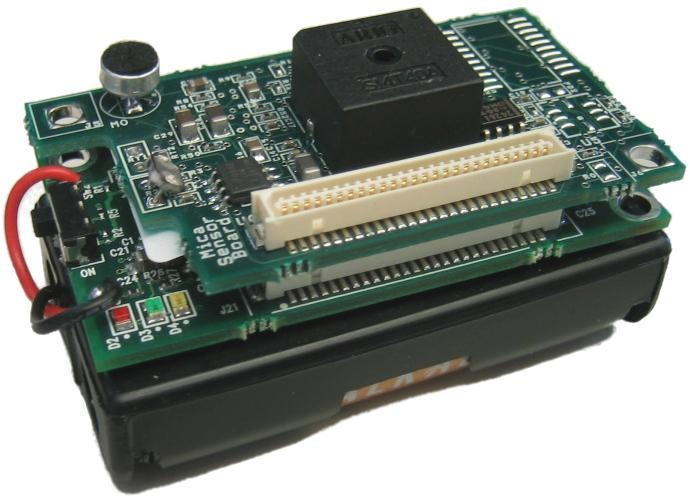
\includegraphics[width=.9\linewidth]{./resources/mica2.jpg}
  \caption{Mica2}
  \label{fig:mica2}
\end{subfigure}
\begin{subfigure}{.24\textwidth}
  \centering
  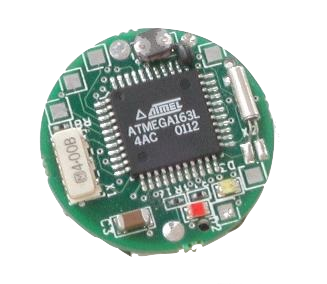
\includegraphics[width=.9\linewidth]{./resources/dot.png}
  \caption{Dot}
  \label{fig:dot}
\end{subfigure}
\begin{subfigure}{.24\textwidth}
  \centering
  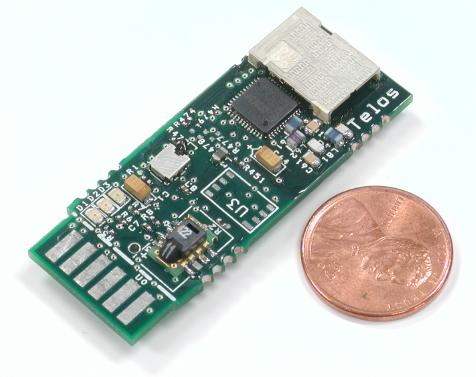
\includegraphics[width=.9\linewidth]{./resources/telos.jpg}
  \caption{Telos}
  \label{fig:telos}
\end{subfigure}
\begin{subfigure}{.24\textwidth}
  \centering
  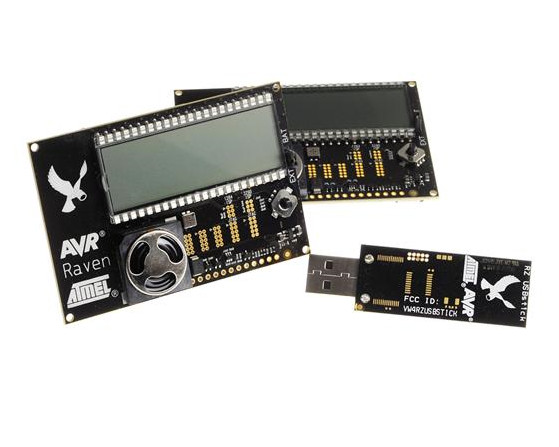
\includegraphics[width=.9\linewidth]{./resources/raven.jpg}
  \caption{AVRraven}
  \label{fig:raven}
\end{subfigure}
\caption{Voorbeelden van sensorknopen}
\label{fig:motes}
\end{figure}

Naast de \mcu heeft een typische sensorknoop tevens een draadloze radio. Je kan
dit vergelijken met de Wi-Fi verbinding die je tegenwoordig in de meeste
computers of smartphones vindt. Voor sensorknopen wordt echter meestal
geopteerd voor een draadloze radio die een minimum aan energie probeert te
verbruiken. Verschillende nieuwe draadloze netwerkstandaarden zijn de laatste
jaren op de voorgrond getreden. De bekendste zijn 6LoWPAN \citep{rfc:6282} en
ZigBee \citep{alliance2012zigbee}. In de volgende paragrafen bekijken we ZigBee
van naderbij; enerzijds omwille van de toepassing in deze masterproef, maar ook
omwille van de voorbeeldfunctie die het kan aannemen voor deze groep van
draadloze standaarden.

\subsection{ZigBee}
\label{subsection:zigbee}

ZigBee zelf is een laag bovenop de netwerklaag gekend als IEEE 802.15.4
\citep{ieee2009802.15.4}. Deze voorziet standaarden op vlak van energiegebruik,
adressering, foutcorrectie, vormgeving van berichten\dots en vormt zo de
fundamenten voor zgn. \emph{low-rate wireless personal area networks}
(LR-WPAN). ZigBee voegt hieraan nog drie belangrijke eigenschappen toe:
routering, ad-hoc netwerkcreatie en zelfherstellende maasnetwerken (\emph{mesh
networks}) \citep{oreilly2010buildingwsn}.

Een ZigBee-netwerk wordt opgebouwd door knopen die elk \'e\'en van drie
verschillende functies kunnen innemen: co\"ordinator, router of eindknoop.

\begin{description}

  \item[Co\"ordinator] Elk netwerk heeft \'e\'en \emph{co\"ordinator}. Deze
  knoop is verantwoordelijk voor het samenbrengen van het netwerk en definieert
  de eigenschappen, bv. met betrekking tot de beveiliging.

  \item[Router] Een \emph{router} stelt andere knopen in staat om met elkaar te
  communiceren. Deze knopen zijn daarom meestal voorzien van een permanente
  stroomvoorziening, omdat ze zich in tegenstelling tot \emph{eindknopen},
  wegens hun communicatieondersteunende rol, niet in een slaapstand kunnen
  zetten.

  \item[Eindkknoop] \emph{Eindknopen}, tot slot, kunnen zich louter verbinden
  met een netwerk, er berichten via versturen en berichten voor zichzelf
  ontvangen. Het is niet de bedoeling om berichten van andere knopen voor
  andere knopen door te sturen. Typisch trachten ze ook hun energieverbruik te
  minimaliseren door hun draadloze radio zoveel mogelijk uit te schakelen.
  Hierdoor worden ze op dat moment onbereikbaar. Het is dankzij \emph{routers},
  die berichten voor de \emph{eindknopen} tijdelijk opslaan, dat ze toch
  berichten kunnen ontvangen.

\end{description}

\subsection{Netwerktopologie en -adressen}
\label{subsection:topologie}

Met knopen kunnen verschillende netwerktopologie\"en gebouwd worden. Figuur
\ref{fig:topologie} geeft een overzicht van de mogelijkheden.

\begin{description}

  \item[Paar] In zijn eenvoudigste vorm bestaat een netwerk uit een
  co\"ordinator en een eindknoop. Deze minimalistische vorm is slechts een
  theoretische mogelijkheid ter volledigheid van de mogelijkheden.
  
  \item[Ster] Wanneer meerdere eindknopen verbonden zijn met dezelfde
  co\"ordinator, vormen zij een stertopologie. Alle communicatie verloopt via
  de centrale co\"ordinator.
  
  \item[Maasnetwerk] In een maasnetwerk worden routers ingeschakeld om
  communicatie via verschillende wegen mogelijk te maken. Eindknopen zijn
  verbonden met deze routers of met de co\"ordinator. Routers en co\"ordinator
  kunnen berichten ontvangen van eindknopen en deze versturen naar andere
  eindknopen, al dan niet via andere routers.
  
  \item[Clusterboom] Een speciale vorm van een maasnetwerk is een clusterboom.
  Hierbij vormen groepen van eindknopen en een router een cluster. De router is
  verbonden met de co\"ordinator, eventueel opnieuw via andere routers, en zo
  wordt een boomstructuur gevormd. De routers die de clusters van eindknopen
  realiseren worden ook clusterhoofden genoemd.
  
\end{description}

\begin{figure}[ht]
  \centering
  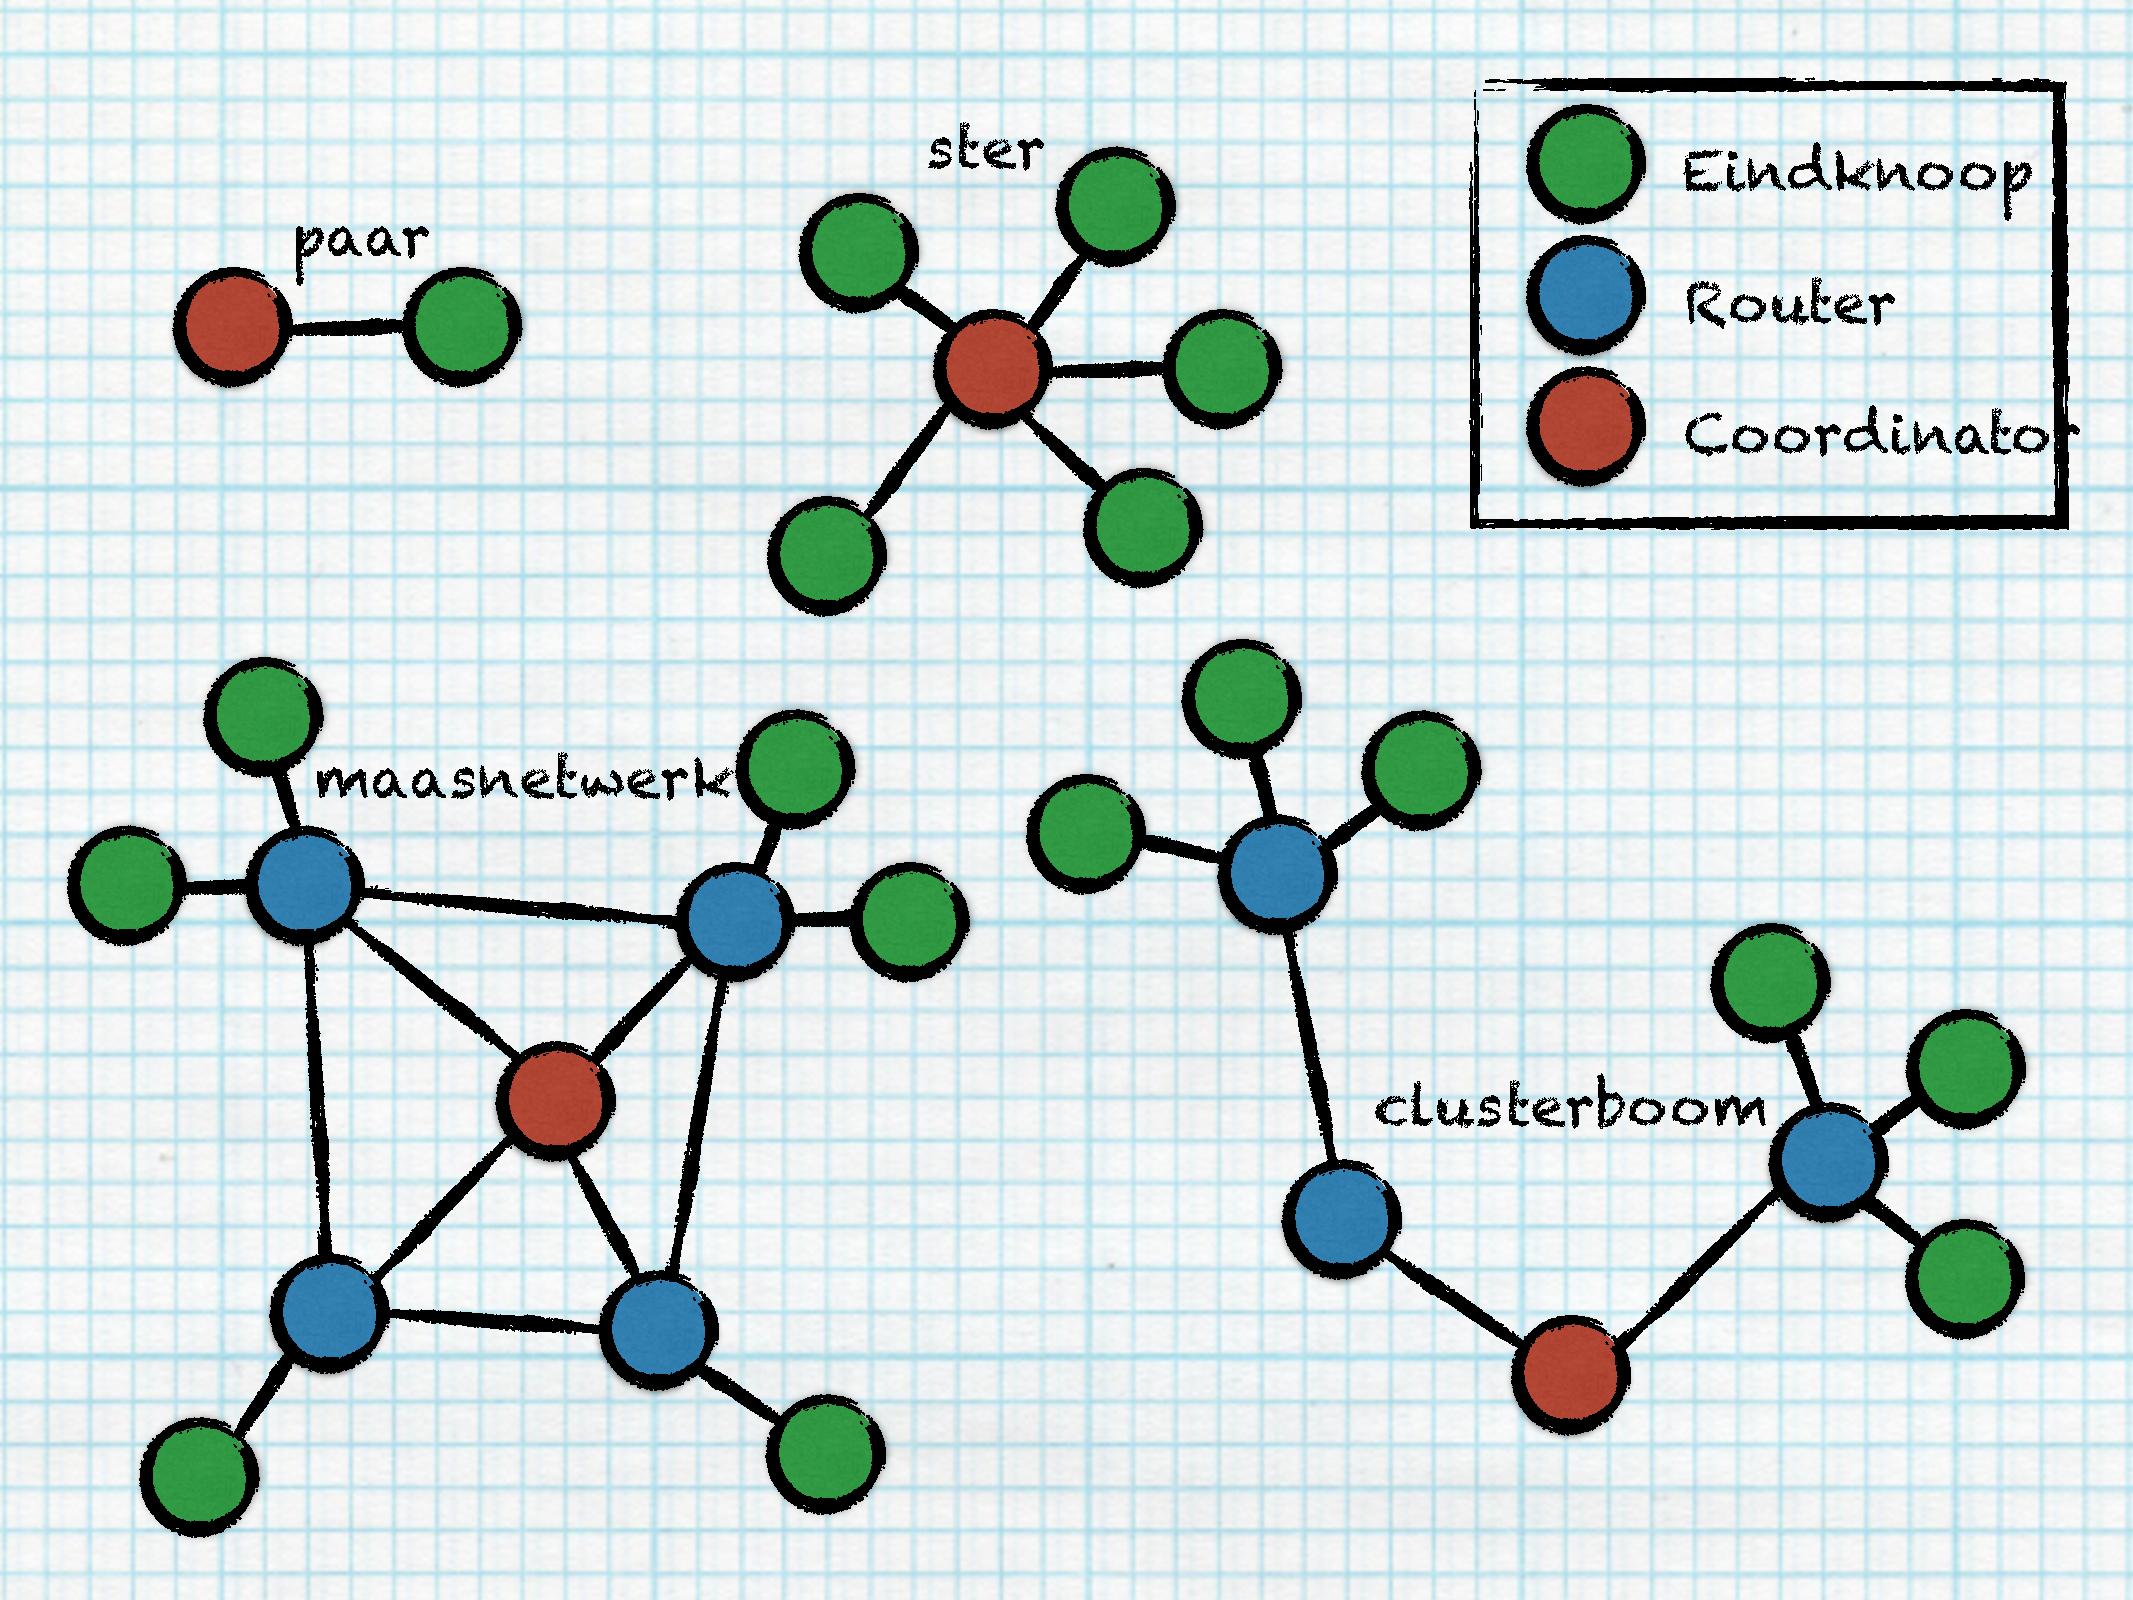
\includegraphics[width=0.7\linewidth]{resources/topology.pdf}
  \caption[Verschillende mogelijke netwerktoplogie\"en]{Verschillende mogelijke
  netwerktoplogie\"en (Bron:\citep{oreilly2010buildingwsn})}
  \label{fig:topologie}
\end{figure}

Het lijkt evident, maar elke knoop, in eender welke topologie, heeft een eigen,
uniek adres, eigenlijk meerdere. Zo heeft een ZigBee-knoop een uniek adres
binnen het netwerk waaraan het deelneemt. Dit adres wordt door de co\"ordinator
van het netwerk toegekend aan een knoop wanneer deze toetreedt tot het netwerk.
Dit \emph{netwerkadres} bestaat uit 16 bits en laat dus toe om 65534 (uit
$2^{16} = 65536$) verschillende adressen toe te kennen. Het adres
\ttt{0x0000}\footnote{We hanteren voor de notatie van adressen de hexadecimale
voorstelling. Elk cijfer stelt een groep van 4 bits voor. 4 groepen stellen zo
een 16 bit adres voor.} reserveert de co\"ordinator voor zichzelf en het adres
\ttt{0xFFFE} wordt typisch gebruikt als het zgn. \emph{broadcast adres}, het
adres waarnaar een bericht gestuurd wordt dat bij alle andere knopen dient
afgeleverd te worden.

Daarnaast heeft elke ZigBee-radio ook een adres dat gegarandeerd overal uniek
is. Dit bestaat uit 64 bits en wordt samengesteld uit twee delen: een eerste
deel beslaat de eerste 32 bits en is voorbehouden voor een unieke identificatie
van de producent. De volgende 32 bits is een uniek nummer binnen de productie
van de producent. Een netwerk zal veelal uit sensoren met dezelfde draadloze
radio's bestaan. Het is daarom logisch dat er gebruik gemaakt wordt van een
\emph{netwerkadres}, dat slechts 16 bits groot is en dus een aanzienlijke
besparing aan geheugen kan opleveren.

Naast de adressen van de knopen is er ook nog het zogenaamde \emph{personal
area network (PAN)} adres. Dit is een unieke identificatie van het netwerk dat
door de co\"ordinator georganiseerd wordt. Ook dit is een 16 bit adres en laat
dus toe om 65536 netwerken op te bouwen.

Tot slot kunnen ZigBee-radio's ook gebruik maken van 12 verschillende
\emph{kanalen}, zodat de volledige adresstructuur bestaat uit een kanaal, een
PAN adres en een netwerkadres.

\section{Beveiligen van sensorknopen}
\label{section:beveiligen}

Het beveiligen van sensorknopen is, in tegenstelling tot de beveiliging van
klassieke computers, bijzonder moeilijk. De computers waar onze emails, foto's
en andere kostbare documenten opgeslagen zijn, zijn uitgerust met een
virusscanner, firewall\dots Dit is mogelijk omdat ze voorzien zijn van een
constante stroomvoorziening, krachtige processor en veel geheugen. Ze worden
tevens fysiek beschermd door ons huis of het datacenter van onze leverancier
van internetdiensten.

In \citep{dargie2010fundamentals} wordt een goed overzicht gegeven van de
uitdagingen die het beveiligen van WSN met zich meebrengen, in vergelijking met
klassieke netwerken. Een sensorknoop heeft geen constante stroomvoorziening en
moet het veelal stellen met een zeer beperkte batterij. Verder ligt de
sensorknoop meestal letterlijk \emph{ten velde} en is hij voor nagenoeg
iedereen fysiek toegankelijk.

Er is ook geen centraal punt waar alle communicatie gegarandeerd passeert. Het
enige communicatiemedium is het draadloze netwerk en via die weg kan men steeds
rechtstreeks contact leggen met elke afzonderlijke knoop, zonder dat de
meerderheid van andere knopen dit ooit merkt. Tot slot is mogen we niet
vergeten dat een draadloos communicatiemedium inherent fouten introduceert, en
dat berichten verloren kunnen gaan.

\subsection{CIA, AAA en andere beveiligingsprincipes}
\label{subsection:cia}

Beveiliging is een zeer ruim begrip dat veel aspecten overspant. Het is
belangrijk dit voor ogen te houden wanneer we over beveiliging spreken.
Theoretische modellen kunnen hierbij helpen. In deze sectie introduceren we
enkele van deze modellen die kunnen helpen om over beveiliging te praten.

Wanneer men spreekt over het beveiligen van computers en netwerken, wordt
dikwijls gerefereerd naar het CIA-beveiligingsmodel. Dit letterwoord staat
voor: vertrouwelijkheid (\emph{confidentiality}), integriteit en
beschikbaarheid (\emph{availability}).

\begin{description}

  \item[Vertrouwelijkheid] Om \emph{vertrouwelijkheid} te garanderen moet
  beveiliging de nodige voorzieningen treffen om er voor te zorgen dat bv. een
  bericht enkel door de bedoelde bestemmeling kan begrepen worden.
  
  \item[Integriteit] Onder \emph{integriteit} verstaat men het principe dat dat
  bericht dan weer niet mag gewijzigd kunnen worden, of dat de bedoelde
  bestemmeling van het bericht ten minste kan valideren dat er aan het bericht
  niets gewijzigd is. 
  
  \item[Beschikbaarheid] Maar beveiliging moet ook de \emph{beschikbaarheid}
  van onderdelen van het netwerk garanderen, om er zeker van te zijn dat dit
  laatste zijn diensten kan blijven aanbieden.

\end{description}

Het CIA-model is zonder meer een belangrijke basis, maar er ontbreken nog veel
belangrijke aspecten. In \citep{rfc:3198} wordt een gestandaardiseerde
terminologie voorgesteld voor het defini\"eren van een beveiligingsbeleid.
Naast de drie hoofdpijlers van het CIA-model vinden we zo ook nog een ander
belangrijk model, namelijk het AAA model voor autorisatie bij
internet-gerelateerde diensten (\emph{triple A}) \citep{rfc:2904}. De afkorting
staat voor authenticatie, autorisatie en vaststellen (\emph{accounting})

\begin{description}

  \item[Authenticatie] Via \emph{authenticatie} kan de identiteit van een
  gebruiker of apparaat vastgesteld worden, zodat eenduidig kan bepaald worden
  van wie bv. een bericht in het netwerk komt.
  
  \item[Autorisatie] \emph{Autorisatie} is daarentegen het proces waarbij
  nagegaan wordt of een gebruiker waarvan de authenticiteit is vastgesteld, een
  bepaalde handeling \emph{mag} uitvoeren.
  
  \item[Vaststellen] Ten slotte biedt het \emph{vaststellen} van alle
  gebeurtenissen en beslissingen binnen het beveiligde domein, een belangrijke
  bron van informatie om een beleid verder te verfijnen en eventueel bij te
  sturen.

\end{description}

In het kader van beveiliging wordt gesproken over een \emph{beleid}
(\emph{policy}), waarin de regels zijn opgenomen waaraan alle spelers binnen
het te beveiligen domein zich dienen te houden. Het AAA-model hanteert een
beleid als zijn centrale gegeven en definieert componenten zoals een
\emph{policy information point} (PIP), \emph{policy decision point} (PDP) en
een \emph{policy enforcement point} (PEP). Deze componenten kunnen aanduiden
waar de verantwoordelijkheid ligt om respectievelijk de juiste informatie aan
te leveren omtrent het beleid, beslissingen te treffen volgens het beleid en
deze beslissingen effectief uit te voeren.

\begin{description}

  \item[Onweerlegbaarheid] Naast deze aspecten, is er ook nog het principe van
  onweerlegbaarheid (\emph{non-repudiation}). Door garanties omtrent
  \emph{onweerlegbaarheid} in te bouwen, kan een ontvanger er zeker van zijn
  dat een zender van een bericht dit bericht effectief verstuurd heeft.

\end{description}

Een aantal gekende technieken bieden klassiek oplossingen voor verschillende
van de hoger vermelde principes: digitale handtekeningen kunnen helpen bij het
garanderen van de \emph{authenticiteit}, \emph{onweerlegbaarheid} en
\emph{integriteit} van een boodschap. Cryptografie kan logischerwijs de
\emph{vertrouwelijkheid} van berichten garanderen, maar kan ook, aan de hand
van publieke en private sleutels, de \emph{authenticiteit} vaststellen.
Berichten kunnen alleen met de andere sleutel van het paar versleuteld worden.

In hoofdstukken \ref{chapter:achtergrond} en \ref{chapter:probleemstelling}
gaan we dieper in op de typische eigenschappen van sensorknopen en belichten we
tal van beveiligingsrisico's waaraan een WSN blootgesteld zijn. Aan de hand van
de zonet beschreven principes zullen we zien dat een WSN inherent moeilijk te
beveiligen is en dat het nagenoeg onmogelijk is om inbraken te vermijden.

\subsection{Inbraakdetectie}
\label{subsection:detection}

Indien het vermijden van inbraken nagenoeg onmogelijk is, moet een belangrijke
tweede beveiligingslinie opgetrokken worden: inbraakdetectie.

Indien we niet weten dat een inbraak heeft plaatsgevonden, zullen we enkel een
vals gevoel van veiligheid hebben. Het is niet omdat we het niet weten, dat ze
er niet zijn. Misschien moeten we zelfs durven stellen dat het belangrijker is
om meer te weten dan te vermijden.

Inbraakdetectie is typisch de stille vennoot in een beveiligingsverhaal. Daar
waar bv. een firewall of authenticatieserver actief toegang ontzegt, zal een
inbraakdetectiesysteem (IDS) typisch geen actieve rol spelen. Het IDS zal
eerder bewijsmateriaal verzamelen om een inbraakpoging te documenteren. Uit
deze informatie kunnen dan bijsturingen aan het beleid aangebracht worden,
waardoor actieve componenten in de toekomst wel in staat zijn om gelijkaardige
inbraakpogingen te verijdelen.

Deze architectuur legt al snel een belangrijk pijnpunt bloot: in een klassiek
netwerk wordt het netwerk beschermd aan de rand. De firewall schermt het
interne netwerk af van aanvallen van buiten. Als een spreekwoordelijke muur van
vuur wordt elke toegang tot het netwerk gelouterd en ongewenste berichten
worden onherroepelijk \emph{verbrand} v\'o\'or ze het netwerk kunnen betreden.

Het IDS wordt daarom typisch ook op het interne netwerk aangesloten daar waar
alle netwerkverkeer dat door de firewall wordt doorgelaten, passeert. Aanvallen
die toch nog door de firewall geraken, kunnen nog door het IDS gedetecteerd
worden.

Dit lijkt op het eerste zicht een tegenspraak. Indien het IDS deze aanvallen
kan detecteren, waarom wordt deze kennis dan niet gebruikt op het niveau van de
firewall? De reden ligt in de natuur van de firewall. Deze werkt immers
hoofdzakelijk op netwerkniveau en bekijkt elk netwerkpakket op zich. Aanvallen
zijn soms een samengang van verschillende pakketten, die typisch op zich zelfs
perfect legaal zijn. Het draait hier hoofdzakelijk om de inhoud van de
pakketten en de analyse vraagt dikwijls een kennis van de toepassingen waarmee
gecommuniceerd wordt. Soms kan slechts aan de inhoud van antwoorden uit het
interne netwerk opgemaakt worden dat er een inbraak plaatsgevonden heeft. Deze
complexiteit is te groot om op het niveau van een firewall te realiseren.

De resultaten van een IDS zullen dikwijls eerder leiden tot verbeteringen aan
de toepassingen binnen het interne netwerk, zodat deze niet meer vatbaar zijn
voor het soort inbraken dat gedetecteerd werd.

Wanneer we dit nu afspiegelen op een WSN, merken we dat enkele fundamentele
principes zo'n architectuur onmogelijk maken: een WSN heeft geen afgebakende
netwerkrand, er is geen uniek punt waar alle netwerkverkeer passeert en waar
een firewall zou kunnen ge\"introduceerd worden, laat staan dat er een manier
zou zijn om al het interne verkeer op \'e\'en enkele plaats te analyseren.

Binnen een WSN is het letterlijk elke knoop voor zichzelf: elke knoop kan
immers van buitenaf benaderd worden zonder dat een aanvaller moet passeren
langs een centraal controlepunt.

\section{Probleemstelling}
\label{section:probleem}

WSN en sensorknopen op zich zijn geen makkelijke klanten wat beveiliging
betreft. Enerzijds hebben ze onvoldoende middellen om zich te beschermen en
anderzijds is hun situatie zo dat het letterlijk elke knoop voor zichzelf is en
dat ze nauwelijks kunnen vertrouwen op hun collega's.

In dit kader moeten gebruikers van een WSN eisen dat er voldoende garanties
worden gegeven zodat ze zich voldoende verzekerd voelen om intieme informatie
toe te vertrouwen aan deze netwerken.

Aangezien het haast onmogelijk is om inbraakpogingen te verijdelen is het van
groot belang dat men in staat is om ze ten minste vast te stellen. Het
introduceren van een IDS in het WSN is echter een directe aanval op de
essenti\"ele functionaliteit van een sensorknoop, waardoor de mogelijkheden
sterk beperkt worden.

\section{Doelstelling}
\label{section:doelstelling}

Zoals we zullen zien in sectie \ref{section:related}, ligt in de literatuur
betreffende ``inbraakdetectie in draadloze sensornetwerken'' de nadruk in
hoofdzaak op het detecteren van specifieke aanvallen of het vaststellen van
anomalie\"en in het verwachte gedrag van sensorknopen en/of het netwerk dat hen
verbindt.

Deze werken stellen tevens dat het een nagenoeg onmogelijke taak is om alle
benodigde detectiemechanismen effectief te implementeren. Dit is logisch,
gegeven de beperkte middelen die sensorknopen ter beschikking hebben. Zo zou
bv. een exhaustieve lijst van aanvalspatronen slechts in sensorknopen met een
groot geheugen opgeslagen kunnen worden en zouden de berekeningen die nodig
zijn om bepaalde anomalie\"en te detecteren gewoonweg te veel energie
verbruiken.

Als in dit stadium van onderzoek naar systemen om inbraken te detecteren het
niet mogelijk is om een sluitend IDS voor een WSN te ambi\"eren, lijkt het
opportuun om een stap terug te zetten en de focus te leggen op de middelen die
nodig zijn om de reeds beschreven, en mogelijk ook toekomstige algoritmen, te
realiseren. Is het mogelijk om een kader te cre\"eren dat een ontwikkelaar van
een sensorknoop in staat stelt om een selectie van de in de literatuur
beschreven oplossingen te implementeren? Kan hij een IDS toevoegen aan zijn WSN
zonder een diepgaande analyse van de onderzoeksliteratuur en zonder zich zorgen
te moeten maken over de onderliggende interactie met andere knopen, het
vergaren en opvragen van informatie op systeem-niveau\dots?

Deze masterproef wil zo'n kader ontwerpen, een prototype implementeren en de
impact bepalen. Daartoe bekijken we eerst enkele typische voorbeelden van
inbraakdetectiealgoritmen, waaruit de functionele en technische vereisten
gedistilleerd worden. Vervolgens stellen we een architectuur voor die aan deze
vereisten kan voldoen. Aan de hand van een prototype gaan we tot slot na wat de
impact is met betrekking tot geheugen, rekenkracht en het gebruik van de
draadloze radio.

De voordelen van een raamwerk zijn legio: een herbruikbaar raamwerk neemt
zorgen, gemeenschappelijk aan de verschillende oplossingen, weg en kan zorgen
voor een betere implementatie. Door middel van een goedgekozen technische
architectuur kan tevens platformonafhankelijheid nagestreefd worden.

%!TEX root=masterproef.tex
\chapter{Achtergrond}
\label{chapter:achtergrond}

In dit hoofdstuk wordt het kader geschetst waarbinnen deze thesis op zoek gaat
naar antwoorden. Enerzijds wordt in sectie \ref{section:landscape} het
landschap van draadloze sensornetwerken in kaart gebracht: wat typeert en
onderscheid hen van andere netwerken? Waarom is het vaststellen van inbreuken
een belangrijk onderzoeksdomein?

Anderzijds wordt in sectie \ref{section:related} ingegaan op een groot aanbod
aan gerelateerd onderzoek. Een belangrijke doelstelling van deze thesis is het
in kaart brengen van de mogelijkheden en beperkingen betreffende reeds
beschreven methodes om inbreuken vast te stellen.

De verschillende beschreven methodes worden gecatalogeerd en gegroepeerd op
basis van verschillende eigenschappen. Op basis van dit overzicht wordt
vervolgens een inschatting gemaakt van de mogelijke dekking die kan bereikt
worden met de bestaande oplossingen.

Bij de beschrijving van de verschillende oplossingen zal tevens kritisch
nagegaan worden in hoeverre de oplossingen in een realistische situatie
effectief bijdragen tot het detecteren van inbreuken in het netwerk.

\section{Draadloze sensorennetwerken}
\label{section:landscape}

\TODO

\section{Gerelateerd onderzoek}
\label{section:related}

\TODO

\subsection{Reputatie en vertrouwen}

De probleemstelling dat knopen in het netwerk elkaar niet langer kunnen
vertrouwen, zette verschillende onderzoekers aan tot het zoeken naar
oplossingen gebaseerd op reputatie en vertrouwen.

\cite{ganeriwal2008reputation} beschrijft een architectuur gebaseerd op
observaties door knopen van de acties van andere knopen in het kader van acties
van zichzelf of derde knopen. Figuur \ref{fig:reputation-cooperation} toont de
situaties die beschouwd worden: in \ref{fig:reputation-cooperative-node} zal
een co\"operatieve knoop (C) alle boodschappen die via hem verzonden worden
door een zendende knoop (Z) effectief doorsturen naar een verder gelegen
ontvangende knoop (O). De verzender van de boodschap, alsook andere naburige
knopen (B) kunnen deze actie vaststellen. In
\ref{fig:reputation-uncooperative-node} daarentegen zal een een
niet-co\"operatieve knoop (NC) deze boodschappen niet verder versturen of zelfs
aanpassen.

\begin{figure}
\centering
\begin{subfigure}{.49\textwidth}
\centering
\[ \entrymodifiers={-=+++[o][F-]}
 \xymatrix@!=0.75pc {
  Z \ar[dr] & *{}       & *{} & *{} \\
  *{}       & C \ar[rr] & *{} & O   \\
  B         & *{}       & *{} & *{} \\
 }
\]
\caption{Co\"operatieve knoop}
\label{fig:reputation-cooperative-node}
\end{subfigure}
\begin{subfigure}{.49\textwidth}
\centering
\[ \entrymodifiers={-=+++[o][F-]}
 \xymatrix@!=0.75pc {
  Z \ar[dr] & *{}       & *{} & *{} \\
  *{}       & NC        & *{} & O   \\
  B         & *{}       & *{} & *{} \\
 }
\]
\caption{Niet-co\"operatieve knoop}
\label{fig:reputation-uncooperative-node}
\end{subfigure}
\caption{Beschouwde situaties bij al dan niet co\"operatieve knopen.}
\label{fig:reputation-cooperation}
\end{figure}

Gegeven knopen $i$ en $j$, met $\alpha_j$, het aantal observaties van acties van
knoop $j$ dat als co\"operatief werd beschouwd, en $\beta_j$, het aantal niet
co\"operatieve acties, toont men aan dat de reputatie van knoop $j$ wordt
weergegeven door een beta distributie van $\alpha_j$ en $\beta_j$:

\begin{equation} \label{eq:reputation-beta}
R_{ij} \sim Beta(\alpha_j+1, \beta_j+1)
\end{equation}

Van deze reputatie kan vervolgens een vertrouwen bepaald worden van knoop $i$
ten opzichte van knoop $j$ als volgt: 

\begin{equation} \label{eq:reputation-trust}
\begin{array}{rcl}
T_{ij} & = & E(R_{ij}) \\
       & = & E(Beta(\alpha_j+1, \beta_j+1)) \\
       & = & \frac{\alpha_j+1}{\alpha_j+\beta_j+2} \\
\end{array}
\end{equation}

$\alpha_j$ en $\beta_j$ evolueren doorheen de tijd. Hierbij dienen enerzijds
nieuwe observaties binnen afzonderlijke tijdspannes beschouwd te worden, maar
moet ook een wegingsfactor toegepast worden op de oude waarden om er voor te
zorgen dat een historisch opgebouwd beeld niet dominant blijft en nieuwe
wijzigingen in het gedrag overstemt. Gegeven $r$ het aantal co\"operatieve
observaties in een bepaalde tijdspanne en $s$ het aantal niet-co\"operatieve
observaties in diezelfde tijdspanne worden de nieuwe waarden voor $\alpha_j$ en
$\beta_j$ gegeven door:

\begin{equation} \label{eq:reputation-update-direct}
\begin{array}{rcl}
\alpha^{new}_j & = & (w_{age} \times \alpha_j) + r \\
\beta^{new}_j  & = & (w_{age} \times \beta_j) + s \\
\end{array}
\end{equation}

Hierbij is $w_{age}$ een factor ($< 1$) die zorgt voor een afname van de
belangrijkheid van de oudere informatie.

Naast deze eigen directe observaties, kunnen ook indirecte observaties door
naburige knopen in beschouwing genomen worden. Voor zo'n naburige knoop, $k$,
zal een knoop $i$ eveneens een vertrouwen $T_{ik}$ kunnen bepalen op basis van
$\alpha_k$ en $\beta_k$. Knoop $k$ kan vervolgens zijn eigen informatie met
betrekking tot de reputatie van knoop $j$ kenbaar maken als $\alpha^k_j$ en
$\beta^k_j$. Knoop $i$ kan vervolgens zijn parameters bijwerken als volgt:

\begin{equation} \label{eq:reputation-update-indirect}
\begin{array}{rrcl}
& \alpha^{new}_j & = & \alpha_j + ( w^k_{rep} \times \alpha^k_j ) \\
& \beta^{new}_j  & = & \beta_j  + ( w^k_{rep} \times \beta^k_j )  \\
met \\
& w^k_{rep}      & = & \frac{2 \alpha_k}{(\beta_k+2) (\alpha^k_j+\beta^k_j+2)+2 \alpha_k} \\
\end{array}
\end{equation}

De factor $w^k_{rep}$ zorgt er voor dat de opname van indirecte informatie van
knoop $k$ in verhouding tot zijn reputatie zal gebeuren.

Enkele bijkomende regels beschermen tegen typische problemen gerelateerd aan
deze aanpak: een knoop accepteert slechts indirecte informatie van een andere,
indien deze knoop zelf als vertrouwd wordt beschouwd. Hierbij wordt een
drempelwaarde ($TH_{SHI}$) gehanteerd. Verder wordt enkel positieve informatie
uitgewisseld, om negatieve be\"invloeding te vermijden. Tot slot wordt tevens
alleen directe informatie uitgewisseld, om de onafhankelijkheid van de
informatie te garanderen.

De auteurs vermelden zelf een zeer belangrijk probleem: omdat knopen constant
moeten luisteren naar de acties van naburige knopen, moeten zij constant actief
zijn. Dit is een zeer nadelig uitgangspunt voor systemen die typisch trachten
zuinig om te springen met hun energie.

Maar de architectuur heeft ook inherente problemen en laat kwaadwillige
partijen toe om - mits kennis van de parameters - net onder de radar te
opereren. We illustreren dit met de simulatie zoals deze uitgevoerd werd door
de auteurs.

De evolutie van een volledige co\"operatieve of volledige niet-co\"operatieve
knoop wordt weergegeven in figuur \ref{fig:reputation-paper}. Een eigenschap
van het algoritme is dat pas na een tiental (louter positieve) observaties een
knoop de drempelwaarde van vertrouwen overschrijdt.

\begin{figure}[h]
\centering
\begin{subfigure}{.49\textwidth}
  \centering
  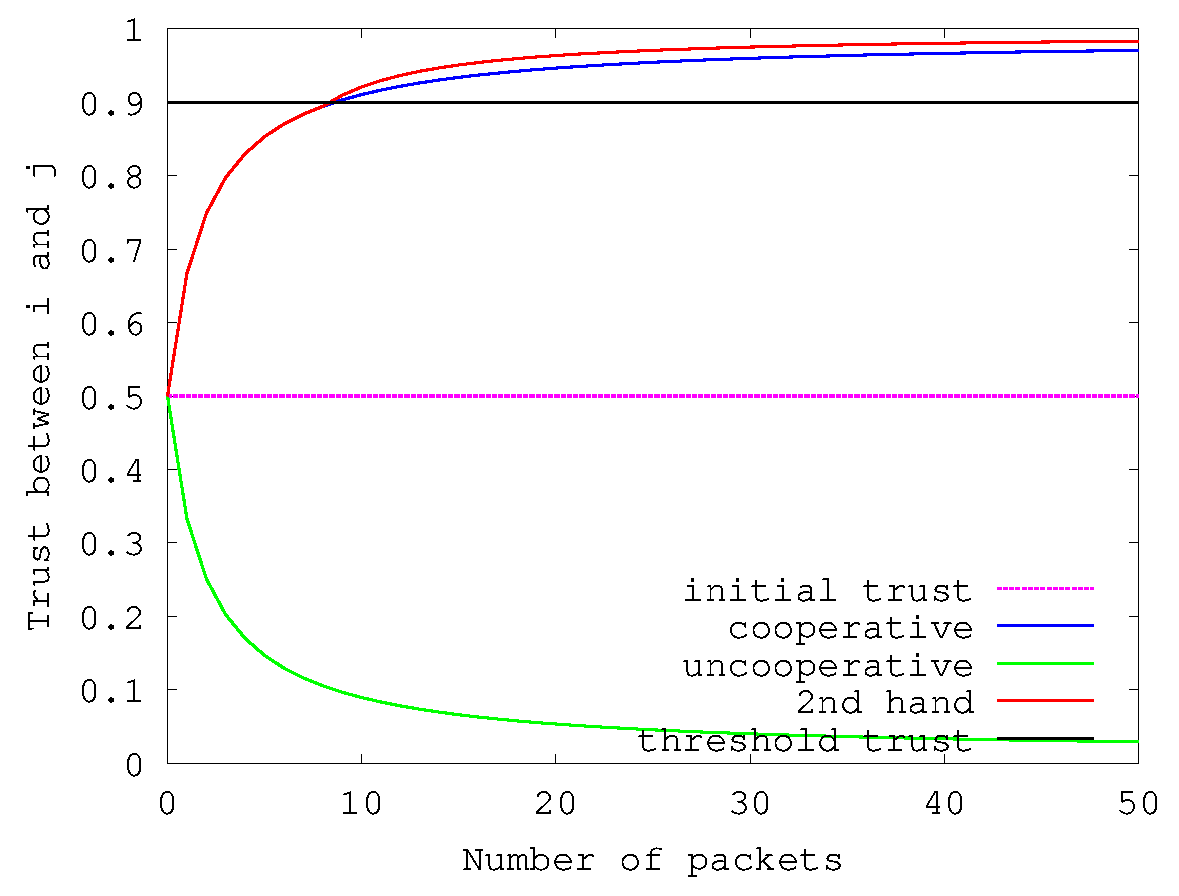
\includegraphics[width=.9\linewidth]{./resources/reputation-paper.eps}
  \caption{Co\"operatieve en niet-co\"operatieve knopen}
  \label{fig:reputation-paper}
\end{subfigure}
\begin{subfigure}{.49\textwidth}
  \centering
  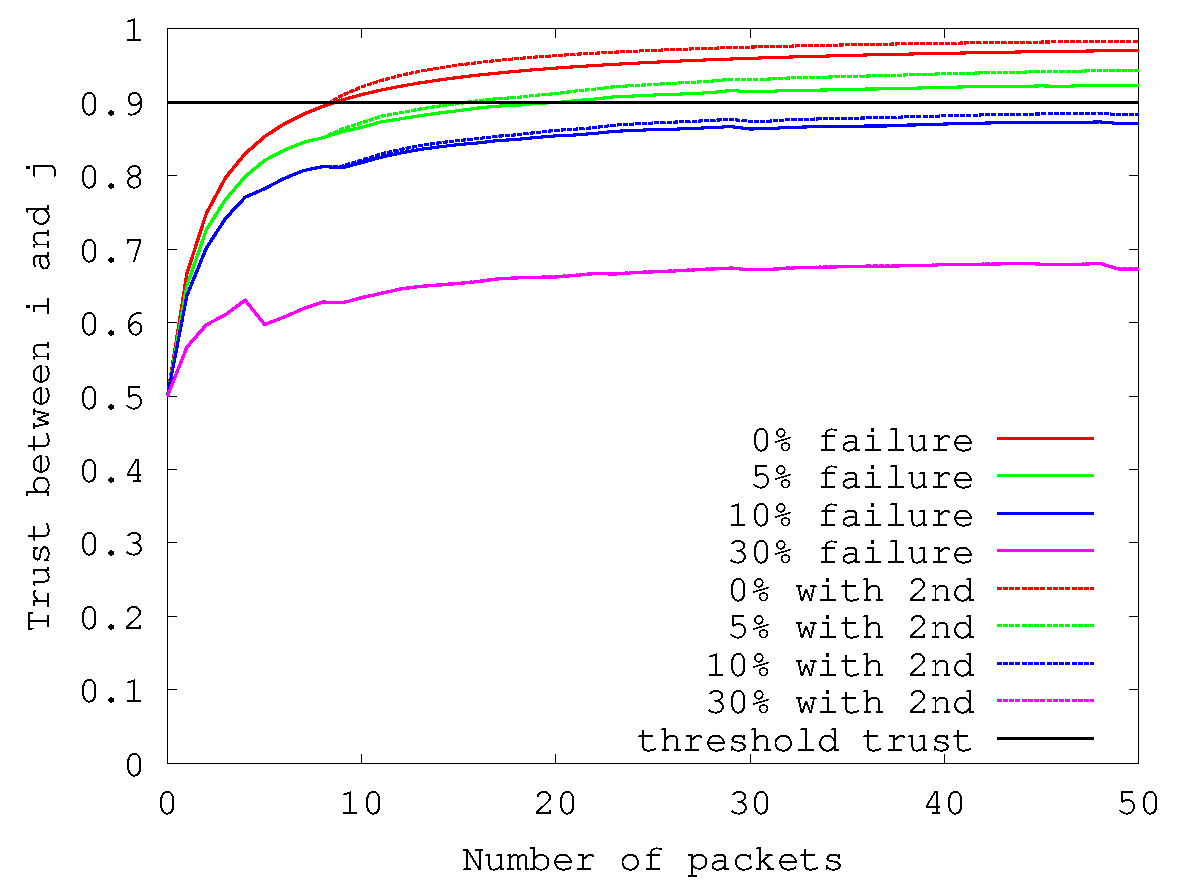
\includegraphics[width=.9\linewidth]{./resources/reputation-with-failure.eps}
  \caption{Falende knopen (100 simulaties)}
  \label{fig:reputation-with-failure}
\end{subfigure}
\caption{Impact van falende knopen op evolutie van vertrouwen.}
\label{fig:reputation-paper-with-failure}
\end{figure}

Deze eigenschap kan echter misbruikt worden zoals aangetoond wordt in figuur
\ref{fig:reputation-with-failure}. Stel dat een knoop $j$ te kampen heeft met
falende hardware, waardoor 5\% van zijn transmissies verloren gaan en daarom
ook niet opgemerkt kunnen worden door andere knopen.

We merken op dat deze knoop, zelfs met 5\% niet-co\"operatieve observaties, na
een twintigtal observaties toch boven de drempelwaarde uitkomt en door de
beschouwende knoop aanvaard wordt als betrouwbaar.

Vanuit een operationeel standpunt gezien is dit in eerste instantie een
positief effect. Indien een node \emph{slechts} 5\% faalt zal deze toch als
co\"operatief beschouwd worden en de goede werking van het netwerk niet
fundamenteel in het gedrang brengen - vanuit een inbraakdetectie oogpunt gezien.

Maar stel dat deze 5\% niet-co\"operatieve acties geen falen zijn en dat de
doorgestuurde boodschappen niet verloren gaan, maar met opzet lichtjes
gewijzigd worden. 5\% kan een significante vertekening van metingen van een
netwerk betekenen en zo de werking van het hele netwerk ondermijnen.

\TODO example of well-crafted malicious behavior

\TODO

\cite{krontiris2009cooperative,castelluccia2009difficulty,krauss2007detecting,seshadri2008sake,maerien2012famos,aschenbruck2012security,afzal2012difisec,yue2012novel,kuang2010snds,blilat2012wireless,ramesh2012wireless,valero2012di,perrig2004security,zhang2000intrusion,djenouri2005survey,yu2008framework,rassam2011novel,da2005decentralized,kachirski2003effective,li2008group,mishra2004intrusion,krontiris2008lidea,ioannis2007towards,soliman2012comparative,wang2011integrated,zhijie2012intrusion}

%!TEX root=masterproef.tex

\chapter{Probleemstelling}
\label{chapter:probleemstelling}

Uit de bespreking van de context waarin deze masterproef kadert, wordt
duidelijk dat inbraakdetectie bij draadloze sensornetwerken een dimensie
complexer kan zijn dan de overeenkomstige oplossingen in een klassiek computer
netwerk. In dit hoofdstuk nemen we het volledige probleemgebied in beschouwing
en duiden we de essenti\"ele pijnpunten aan.

De wereld van DSN bestaat uit meer dan louter de sensorknopen, maar ze vormen
wel het uitgangspunt. In sectie \ref{section:problem-hardware} vertrekken we
van de hardware en het netwerk waar het deel van uitmaakt.

\'E\'en niveau boven de hardware vinden we de software die de sensorknoop in
staat stelt om zijn taken uit te voeren. In sectie
\ref{section:problem-software} bekijken we deze software, waarbij o.a.
besturingssystemen aan bod komen.

De eerste stap  in ontwikkeling van software  is de analyse van  het probleem en
een beschrijving van de beoogde  implementatie. In het geval van inbraakdetectie
in  DSN, moeten  we ons  hiervoor nog  beroepen op  onderzoeksliteratuur. Sectie
\ref{section:problem-research} bekijkt  daarom de situatie van  onderzoekers. De
volgende  stap wordt  genomen in  sectie \ref{section:problem-develop},  waar we
focussen op de ontwikkelaar.

Tot slot is de ontwikkelaar zelden de eigenaar of uitbater van het netwerk. Op
het hoogste niveau vinden we de persoon die uiteindelijk de reden is van het
bestaan van de sensorknopen, de software en het netwerk als een geheel. De
problemen op het niveau van de uitbating worden bekeken in sectie
\ref{section:problem-operations}.

\section{Sensorknopen}
\label{section:problem-hardware}

Sensorknopen en een DSN in het algemeen lijken op het eerste zicht slechts een
zoveelste variant van een mobiel en ad-hoc netwerk (MANET)
\citep{garg2010mobile}, waarvan de beveiligingsrisico's reeds uitvoerig
onderzocht zijn \citep{djenouri2005survey, zhang2000intrusion,
kachirski2003effective}, toch blijkt al snel dat een DSN nog enkele typische
eigenschappen heeft die de problematiek uitvergroten.

In \citep{garg2010mobile} vinden we een beknopte maar duidelijke vergelijking
van een MANET versus een DSN:

\begin{itemize}

  \item Het aantal knopen in een DSN is veel groter dan het aantal
  participanten van een MANET. Typische grootorde is 1.000 tot 10.000 knopen
  over de betrokken oppervlakte.

  \item Sensorknopen zijn meestal immobiel en moeten samenwerken om de
  gedetecteerde gegevens te verzenden.

  \item In een MANET is het aantal knopen veel lager, maar hun mobiliteit is
  zeer hoog.

  \item Sensorknopen gebruiken hoofdzakelijk het \emph{broadcast} paradigma om
  te communiceren, waar in een MANET punt-naar-punt communicatie wordt gebruikt.

  \item Op vlak van energieverbruik, merken we dat sensorknopen een veel lager
  verbruik kennen; typisch rond de 0,75 mW.

\end{itemize}

Uit de verschillen begrijpen we dat een DSN makkelijker kan aangevallen worden
door zijn opbouw uit een groot aantal statische knopen, die typisch via
\emph{broadcasting} communiceren. Aangezien dat zich telkens slechts een kleine
subgroep van het netwerk binnen een actieve communicatieradius bevindt, maakt
dat grote delen van het netwerk \emph{blind} of eerder \emph{doof} zijn voor
wat er zich afspeelt.

Hierbij komt dat, om het energieverbruik laag te houden, sensorknopen typisch
trachten om zoveel mogelijk in een slaaptoestand te vertoeven. Hierdoor worden
de omringende knopen nog meer ontzegt van enige samenwerking. We merken hier op
dat er een onderscheid gemaakt moet worden tussen de beschikbaarheid van een
sensorknoop en de beschikbaarheid van het netwerk als een geheel en dat niet
eenvoudig een sensorknoop op zich mag beschouwd worden wanneer we een analyse
zouden maken van het beveiligingsrisico.

Bijlage \ref{appendix:node-capture} toont hoe eenvoudig het is om \'e\'en enkele
knoop te veroveren wanneer fysieke toegang mogelijk wordt, waardoor we moeten
uitgaan van het feit dat geen enkele in het geheugen opgeslagen informatie per
definitie veilig is. Hier zien we dat op valk van integriteit, een sensorknoop
zeer kwetsbaar is en dat informatie die gebruikt kan worden voor authenticatie
al snel publiekelijk kan worden.

Daartegenover staat echter wel dat door het grote aantal knopen, een louter
fysieke aanval meestal onmogelijk is. Een aanvaller kan wel door een enkele
knoop te veroveren zichzelf toegang tot het netwerk verlenen, toch zal het
vervolg van de aanval zich meer op een functioneel niveau afspelen. Op dat
ogenblik komt het grote aantal knopen in het netwerk tot zijn recht. De
\emph{buren} van een veroverde knoop, kunnen samenwerken zoals we zagen in
sectie \ref{subsection:cooperation}, om een eventuele indringer te ontmaskeren.

Indien de aanvaller inderdaad een knoop heeft veroverd en wijzigingen heeft
aangebracht aan de software om zo gebruik te kunnen maken van de knoop binnen
het netwerk, kan zoals we zaken in sectie \ref{subsection:attestation} software
attestatie een mogelijke piste zijn voor naburige knopen om indringers te
detecteren.

Maar veelal zullen de knopen in een DSN zich moeten focussen op het detecteren
van anomali\"en in het gedrag van andere knopen, eerder besproken in sectie
\ref{subsection:anomaly}. Aangezien een knoop niet heel de tijd actief is en
dus niet alle gedragingen van andere knopen kan aanschouwen, kan er ook geen
sprake zijn van een totaalbeeld en zal een knoop slechts een statistische
zekerheid kunnen opbouwen omtrent het vertrouwen dat geschonken wordt aan een
andere knoop. Algoritmen die zulk een reputatie ondersteunen zagen we eerder in
sectie \ref{subsection:reputation}.

Omdat een DSN grote hoeveelheden gegevens verzameld, is een reductie en
tussentijdse verwerking soms een noodzaak. Dit maakt natuurlijk ook dat
tussenliggende knopen de gegevens die via hen verstuurd worden moeten kunnen
verwerken. Klassieke encryptie tussen verzender en ontvanger is in het geval
een DSN dus niet echt aangewezen. Terugvallen op een symmetrische sleutel is
een optie, maar plaatst de vertrouwelijkheid onder druk.

Een andere systeem, bv. met publieke sleutels, zal veelal te zwaar uit vallen,
omdat de algoritmen enerzijds een te grote belasting zouden vormen voor de
rekenkracht en zo ook het energieverbruik zouden taxeren. Anderzijds zou de
hoeveelheid sleutels die elke knoop zou moeten beheren de geheugennoden de
hoogte in drijven. Dit zorgt natuurlijk ook voor een probleem omtrent
niet-weerlegbaarheid. Dit probleem is natuurlijk een belangrijk
onderzoeksdomein. De auteurs van \citep{girao2005cda} stellen met
\emph{Concealed Data Aggregation} (CDA) een oplossing voor die encryptie van
verzender tot ontvanger garandeert, maar tevens toelaat dat tussenliggende
knopen de informatie aggregeren, zonder deze te decoderen.

We kunnen concluderen dat sensorknopen en -netwerken duidelijk geen eenvoudige
omgeving zijn wanneer het neerkomt op beveiliging. Ze slagen er in om ongeveer
tegen elk aspect van zowel het CIA als AAA model in te gaan, wat zich tevens
reflecteert in het feit dat ze tegelijkertijd de rol vervullen van PDP en PEP.
De rol van PIP is gedistribueerd. Elke node is in eerste plaats zijn eigen PIP,
waardoor alle rollen samenvallen. Anderzijds kunnen inbraakdetectiealgoritmen
ook informatie van andere knopen gebruiken, zoals we zagen in het geval van
reputatie in sectie \ref{subsection:reputation}. Gegeven de problematische
eigenschappen hierboven beschreven, moet deze informatie natuurlijk steeds met
de nodige argwaan behandeld worden.

\section{Software}
\label{section:problem-software}

In een normale situatie wordt er uit gegaan van een solide basis en wordt het
hardware-platform en het netwerk gezien als een veilig vertrekpunt. Software
wordt vervolgens typisch gezien als het zwakke broertje waar allerhande kleine
fouten leiden tot inbraakmogelijkheden.

De typische werking van een sensorknoop bestaat uit het herhaaldelijk uitvoeren
van dezelfde taken: ondervragen van sensoren voor meetgegevens, deze
meetgegevens doorsturen naar een centraal punt en berichten van andere knopen
verder doorsturen. De software lijkt eenvoudig, maar dit durft bedrieglijk te
zijn. Er zijn immers veel situaties waar de werking niet zo eenvoudig of
sequentieel verloopt als de beperkte functionaliteit laat uitschijnen. Terwijl
de knoop zijn sensoren benadert kan er een boodschap van een andere knoop
toekomen, of de knoop waarnaar een bericht verzonden moet worden is niet
beschikbaar, enz.

Ook al is de functionaliteit redelijk beperkt, toch dient met voor het
schrijven van software voor sensorknopen, al snel terug te vallen op software
bibliotheken en/of raamwerken om enkele typische gebruikspatronen te
ondersteunen en toegankelijk te maken. Ook besturingssystemen worden ontwikkeld
voor sensorknopen. Ze kunnen niet vergeleken worden met klassieke
besturingssystemen. Het zijn typisch uitgebreide raamwerken die diensten
leveren zoals procesbeheersing, geheugengebruik, netwerkcommunicatie,enz. Twee
leidende voorbeelden zijn TinyOS \citep{levis2005tinyos} en Contiki
\citep{dunkels2004contiki}.

Het is duidelijk dat beide kiezen voor een aanpak die gericht is op de
ontwikkeling van toepassingen: TinyOS zet sterk in op componenten en Contiki op
lichte processen, het dynamische laden van modules en was een voorloper met
\'e\'en van de eerste IPv6 netwerkimplementaties. Het is niet de bedoeling van
deze masterproef om een gedetailleerde vergelijking te maken van beide. We zien
zelfs dat ze naar elkaar toegroeien. Voor een gedetailleerdere vergelijking
verwijzen we naar \citep{reusing2012comparison} en delen de conclusie dat beide
besturingssystemen in staat zijn om de typische noden van een sensornetwerk te
ondersteunen. De verschillen zitten in details, waarbij TinyOS typisch beter
uitgerust is wanneer de beschikbare middelen echt schaars zijn. Contiki
daarentegen biedt meer flexibiliteit en is daarom soms een betere keuze als de
software van de knoop regelmatig moet bijgewerkt worden en dit voor een groot
aantal knopen.

Aangezien beveiliging niet aan de basis ligt van deze systemen, vinden we
hieromtrent veel onderzoek \citep{paul2009safe, casado2009contikisec,
karlof2004tinysec}. Dit is echter een suboptimale situatie. Desalniettemin zijn
deze systemen een noodzakelijk kwaad.

\section{Onderzoek}
\label{section:problem-research}

De problemen met de interactie met het platform en de taal, brengen ons bij de
menselijke kant van het probleem. We volgen het ontwikkelingsproces van begin
tot einde en starten daarom dicht bij huis met het onderzoek naar
detectiealgoritmes.

De bespreking van gerelateerd onderzoek in sectie \ref{section:related} is
slechts een kleine bloemlezing van de totaliteit aan literatuur die de
afgelopen jaren geproduceerd is. Toch is \'e\'en teneur duidelijk aanwezig: de
onmogelijkheid om een sluitend geheel te bouwen hangt als een zwaard van
Damocles boven elke voorgestelde oplossing.

En dit heeft wel degelijk ingrijpende gevolgen voor onderzoek. De meerderheid
aan artikels focust zich op een klein detail, een oplossing voor \'e\'en
specifiek probleem. Slechts een minderheid durft een raamwerk voor te stellen,
echter geen enkel biedt een open uitnodiging om ander onderzoek echt op te
nemen. Er is geen basis om inbraakdetectiealgoritmes voor DSN op formele manier
uit te werken.

Dit leidt tot veel literatuur, met intrinsieke waarde, maar die bijzonder
moeilijk te evalueren, laat staan te implementeren is. Maar deze situatie is
evengoed nadelig voor de onderzoekers zelf. Zo zijn ze nauwelijks in staat om
hun werk effectief te evalueren of zelfs te vergelijken. Resultaten worden
louter gebaseerd op specifieke implementaties en maken geen abstractie van het
platform. Veelal zijn ze zelfs specifiek ontworpen voor \'e\'en specifiek
platform en is de overdraagbaarheid een groot vraagteken.

Ook indien er gewerkt wordt met simulaties, zijn deze meestal zeer
platform-gebonden en zijn de resultaten eerder technisch dan functioneel van
aard. Van interoperabiliteit is nagenoeg geen sprake en niet \'e\'en artikel
werd gevonden waar werken van verschillende auteurs samen worden gebracht.

\section{Ontwikkeling}
\label{section:problem-develop}

Deze literatuur vormt de basis waarvan ontwikkelaars dienen te vertrekken. Uit
de enkele voorbeelden die we eerder zagen, kunnen we reeds opmaken dat zelfs de
elementairste algoritmen toch al aardig wat werk met zich meebrengen.
Vermenigvuldig dat met een aantal algoritmen om een redelijke dekking te
bekomen en het werk om een IDS te voorzien overstijgt het effectieve
functionele sensor-gerelateerde werk dat feitelijk de enige bedoeling is van de
ontwikkeling.

In tegenstelling tot andere takken van de informatica en software ontwikkeling,
kan er in het geval van inbraakdetectie in een DSN, geen gebruik gemaakt worden
van bestaande implementaties en kan een ontwikkelaar niet eenvoudig een
bibliotheek importeren en met een eenvoudige oproep een detectiealgoritme
toevoegen aan zijn toepassing. In de voorgaande sectie zagen we waarom het
onderzoek hier geen bruikbaar materiaal aanlevert.

Indien \'e\'en van de drijfveren van ontwikkelaars is om de levensduur van een
enkele batterij optimaal te benutten, is het eenvoudig hergebruiken van
bestaande bibliotheken van algoritmen geen optie. De verschillende algoritmes
voeren typisch dezelfde operaties uit: verwerken van inkomende berichten, het
overlopen van gekende knopen \dots

Ook de C programmeertaal is op zich al een uitdaging. Dit heeft geleid tot
nader onderzoek en verschillende gespecialiseerde talen hebben reeds hun
opwachting gemaakt. Een eerste zagen we reeds in de context van TinyOS, dat
nesC \citep{gay2003nesc} gebruikt, een component-geori\"enteerde uitbreiding
van C. Binnen het zelfde project werd ook TinyScript
\citep{levis2004tinyscript} ge\"introduceerd; een imperatieve, op Basic
ge\"inspireerde taal met dynamische typering en elementaire controle structuren
zoals condities en lussen. De doelstelling is om de complexiteit van de
onderliggende nesC taal te verbergen voor minder technische analisten.

Maar ook fundamenteel andere talen trachtten een antwoord te bieden voor de
discrepantie tussen de relatief lage complexiteit van de toepassing en
detectiealgoritmen en de soms complexe implementatie binnen een op momenten
barbaarse ontwikkelomgeving. \'E\'en van de doelstellingen van het ABSYNTH
project \citep{url:absynth} is om domein experten controle te geven over de
ontwikkeling van software voor DSN. Om dit te realiseren hanteren ze talen,
compilers en synthese technieken. WASP2, een taal die ontworpen werd in het
kader van dit project, is \'e\'en uit een aantal talen die opteerden om
database-geori\"enteerde talen als voorbeeld te nemen.

\section{Uitbating}
\label{section:problem-operations}

Het belang van de controle door domein experten brengt ons bij een laatste
groep mensen die toch graag controle wil hebben over een DSN: de eigenaar of
uitbater van het netwerk.

Het beeld dat de eigenaar een \'e\'enmalige opdracht geeft tot ontwikkeling kan
misschien te verdedigen zijn in projecten waar weinig tot geen beveiliging
genoodzaakt is, maar bij meer kritische applicaties waar er effectief een IDS
voorzien wordt in het netwerk, is dit zeker niet meer van toepassing.

Een IDS kan, zeker in het kader van een DSN, geen statisch gegeven zijn. De
uitbater van een netwerk zal, indien het inzetten van een IDS serieus wordt
genomen, genoodzaakt zijn om de set van algoritmen over tijd aan te passen.
Wanneer we bv. nogmaals kijken naar SNORT \citep{roesch1999snort}, dan zien we
dat ook bij deze centrale IDS er regelmatige updates gebeuren van de patronen
die gedetecteerd kunnen worden. Dit zal niet anders zijn bij een IDS in een DSN.

Indien de uitbater voor elk van deze aanpassingen terug moet gaan naar de
ontwikkelaar, zal dit snel een onwerkbare en vooral onrealistische situatie met
zich meebrengen. Een uitbater moet in staat zijn om op een flexibele manier het
IDS van zijn DSN te configureren en te voorzien van nieuwe of bijgewerkte
detectiealgoritmen. Net zoals een klassiek IDS, zou een IDS voor een DSN
eigenlijk als een aparte entiteit moeten kunnen beheerd worden.

%!TEX root=masterproef.tex

\chapter{Oplossingsstrategie}
\label{chapter:oplossingsstrategie}

Uit de probleemstelling moeten we concluderen dat er weinig in het voordeel van
het bouwen van een IDS voor een WSN spreekt. Op elk niveau, van de hardware van
de knoop en de elementaire software die het netwerk vormgeeft, tot de
onderzoeker, ontwikkelaar en uitbater van het netwerk, zijn er obstakels te
identificeren. Dit hoofdstuk volgt opnieuw de verschillende stappen in de keten
en tracht een antwoord aan te bieden dat tegemoet komt aan de
ge\"identificeerde problemen.

Sectie \ref{section:solution-node-wsn} stelt dat het ontbreken van een dominant
hardwareplatform er toe leidt dat de oplossing flexibel moet zijn t.o.v.
verschillende platformen.

Sectie \ref{section:solution-software} veralgemeent deze eis naar het niveau
van de software, omdat er bv. ook geen overheersend besturingssysteem
beschikbaar is.

Sectie \ref{section:solution-proglang} evalueert de mogelijkheid om de
programmeertaal C te hanteren als gemeenschappelijke en gestandaardiseerde taal
om detectiealgoritmen te beschrijven.

Sectie \ref{section:solution-library} introduceert softwarebibliotheken als een
oplossing voor gemeenschappelijke logica en het centraliseren van iteratieve
processen.

Sectie \ref{section:solution-dsl} argumenteert dat een domeinspecifieke taal
een oplossing kan zijn om aan de hand van een formele en platformonafhankelijke
beschrijving van algoritmen o.a. een brug te slaan tussen onderzoek en
ontwikkeling.

Sectie \ref{section:solution-codegen} tot slot stelt dat codegeneratie een
geformaliseerd proces kan automatiseren en kan tegemoet komen aan de overige
problemen in het kader van het ontwikkelingsproces.

\vspace{-3mm}

\section{Hardware en netwerk}
\label{section:solution-node-wsn}

Het feit dat sensorknopen, en ge\"integreerde systemen in het algemeen, fysiek
toegankelijk zijn en daarom inherent vatbaar voor fysieke aanvallen, is een
probleem waaraan op zich weinig kan gedaan worden. Zolang de ontwikkeling van
sensorknopen in zijn kinderschoenen staat en de focus nog op de basisbehoeften
ligt (energiebesparing, grootte,...) en zolang er geen echte standaard voor
deze hardware bestaat\footnote{Standaarden zullen zonder twijfel ontstaan en de
eerste schuchtere pogingen zijn reeds te zien in de vorm van bv. het Zigduino
platform (\url{http://www.logos-electro.com/store/zigduino-r2}) of de Waspmote
van Libellum (\url{http://www.libelium.com/products/waspmote/}).}, zal het nog
even duren voor de focus verschuift naar de beveiliging van de hardware.

Vanuit het oogpunt van de hardware en het netwerk houden we daarom een
belangrijk criterium voor ogen: de oplossing moet flexibel genoeg zijn om met
verschillende soorten hardware, netwerkprotocollen\dots om te gaan en mag dus
niet inherent afhankelijk zijn van beperkende veronderstellingen op dit niveau.

\vspace{-3mm}

\section{Elementaire software}
\label{section:solution-software}

Onder elementaire software verstaan we elke vorm van software die nodig is om
de basisbehoeften van het systeem te vervullen. Daarbij denken we aan een
besturingssysteem, maar dat verschilt van de klassieke opvatting in het geval
van een sensorknoop, bv. in grootte en mogelijkheden. Maar het kan ook zo
eenvoudig zijn als een eindeloze herhaling van dezelfde instructies.

Een besturingssysteem voor een sensorknoop biedt een dunne abstractielaag die
de harde realiteit van de programmatie van een naakte \mcu verlicht door de
introductie van processen, componenten\dots Gegeven de beperkte voorzieningen
van een sensorknoop, focust de ontwikkeling van deze systemen zich op het
beperken van de eigen impact en zal daarom zoveel mogelijk balast trachten te
vermijden.

De meeste van deze systemen zijn openbronsoftware en integratie is mogelijk
door diepgaande aanpassingen. Aanpassingen zijn dan wel nodig voor elk
besturingssysteem en net zoals bij de hardware, is er nog geen de facto
standaard. TinyOS en Contiki zijn zonder twijfel sterke spelers, maar de
\emph{Windows} onder de besturingssystemen voor sensorknopen moet nog opstaan.

\vspace{-3mm}

\section{Programmeertalen}
\label{section:solution-proglang}

De keuze van een programmeertaal gaat in het geval van een WSN vooral samen met
de taal die gebruikt wordt door het besturingssysteem. Omdat dit systeem
typisch niet op zich staat en de toepassing samen met het systeem tot een
geheel verwerkt wordt, is de integratie tussen de twee zeer sterk.

De ontwikkelaar van de hardware levert bij zijn sensorknopen, of zelfs al bij
een \mcu, typisch \'e\'en compiler en derhalve ook \'e\'en taal. Het aanbod is
uitermate beperkt en bestaat in grote lijnen uit ``C''. Er bestaan
alternatieven, maar die zijn schaars, bv. de SunSpot van Oracle, die Java
aanbiedt.

De programmeertaal C staat zeer dicht bij de hardware en is duidelijk de eerste
stap in de ontplooiing van softwareontwikkeling op ge\"integreerde systemen. De
voorzichtige pogingen om nieuwe programmeertalen voor te stellen tonen aan dat
op dit vlak een evolutie in ontwikkeling is. Maar het zal nog enige tijd duren
vooraleer een nieuwe, dominante taal opstaat en C van de troon stoot.

Op dit ogenblik is C de lingua franca voor alle spelers in dit segment: zowel
onderzoeker als ontwikkelaar hanteren deze taal, ook al moet de kanttekening
gemaakt worden dat in veel gevallen onderzoekers zich nog beroepen op
simulaties waarbij C ontweken wordt.

\vspace{-3mm}

\section{Softwarebibliotheek}
\label{section:solution-library}

In sectie \ref{section:problem-develop} zagen we reeds dat \'e\'en van de
pijnpunten is dat de verschillende algoritmen typisch dezelfde acties
ondernemen. Indien de algoritmen als onafhankelijke modules zouden worden
ontwikkeld en sequentieel achter elkaar opgeroepen worden, zullen zij veel
dubbel werk leveren. Dat gaat echter ten koste van de energievoorziening en dus
de levensduur van de knoop.

Dit is een klassiek softwareprobleem en wordt normaal opgevangen door het
gebruik van een softwarebibliotheek. Deze biedt een verzameling van functies
die toelaten om gemeenschappelijke functionaliteit slechts \'e\'enmaal te
defini\"eren en vervolgens vanuit specifieke toepassingen of algoritmen aan te
spreken.

De introductie van een softwarebibliotheek lost een aantal van de technische
problemen op, maar zal weinig dekking geven voor de overige aspecten. Zo moeten
bij gebruik van een softwarebibliotheek de regels ervan ook effectief gevolgd
worden door alle partijen. De analyse van onderzoeksdocumenten en het koppelen
aan de gebruikte softwarebibliotheek blijft nog steeds een dure en
foutgevoelige taak.

Zelfs indien men bij onderzoek gebruik zou maken van dezelfde
softwarebibliotheek, zou dit nog niet platformonafhankelijk zijn, zou de taal
vastliggen en zou ook bv. het netwerkprotocol of zelfs de sensorknoop
vastliggen. Buiten het feit dat de ontwikkeling makkelijker en beter zou kunnen
gebeuren, levert het geen enkel voordeel op voor de onderzoekers.

\vspace{-3mm}

\section{Domeinspecifieke taal}
\label{section:solution-dsl}

Indien de programmeertaal en een softwarebibliotheek nog te veel vrijheid laten
en geen integratie van onderzoek en ontwikkeling kunnen bewerkstelligen, kan er
gekeken worden naar een andere gemeenschappelijke taal om de algoritmen in uit
te drukken. In klassieke softwaremethodologie\"en wordt hiervoor bv.
\emph{Unified Modeling Language} (UML) \citep{url:uml} of een andere
analysetaal gebruikt.

In het geval van inbraakdetectie voor een WSN, zou de keuze kunnen vallen op
een domeinspecifieke taal (\emph{Domain Specific Language})
(DSL)\citep{van2000domain, mernik2005and, fowler2010domain}. Het domein,
inbraakdetectie in draadloze sensornetwerken, is immers duidelijk afgelijnd en
is beperkt in functionaliteit: knopen kunnen berichten ontvangen en versturen
alsook metingen doen aan de hand van hun sensoren.

Domeinspecifieke talen kunnen veel vormen aannemen. Zo zijn er \emph{inwendige}
talen die binnen een bestaande programmeertaal kunnen gebruikt worden. Ze
gebruiken de mogelijkheden van de omkaderende taal en omgeving om een
bijkomende taal te realiseren die voordelen biedt bovenop het gebruik van de
basistaal. Het is duidelijk dat de keuze voor een inwendige DSL samengaat met
de mogelijkheden van de overkoepelende programmeertaal. De implementatie van
een inwendige DSL in C is mogelijk, maar zal slechts een beperkte meerwaarde
bieden. Daartegenover staat trouwens dat we met een inwendige DSL geen
beperkingen kunnen opleggen aan de omkaderende taal. Alle mogelijkheden van C
zouden ter beschikking blijven en ongewenste constructies zouden nog steeds
kunnen binnendringen.

Een tweede groep van talen zijn de zgn. \emph{uitwendige} talen. Dit zijn talen
die onafhankelijk van een programmeertaal opgebouwd worden en dus volledig vrij
zijn in het bepalen van restricties en mogelijkheden. Een uitwendige DSL kan in
het geval van inbraakdetectie een oplossing zijn om de beschrijving van
detectiealgoritmen te formaliseren. Zo'n beschrijving kan platformonafhankelijk
zijn, waardoor de resultaten van onderzoek direct herbruikbaar en breed
toepasbaar worden.

Door de DSL te laten aansluiten bij C en uit te breiden met constructies die
toelaten om op een hoger niveau met gegevensstructuren om te gaan, ontstaat een
omgeving die zeer nauw aansluit bij zowel onderzoekers als ontwikkelaars.

\vspace{-3mm}

\section{Codegeneratie}
\label{section:solution-codegen}

Eens men beschikt over een formele beschrijving van een algoritme, is de stap
naar codegeneratie niet meer groot. Codegeneratie is geen noodzakelijke stap,
maar blijkt in dit kader toch een meerwaarde.

Zo kan een uitbater van een WSN zelf de software voor zijn netwerk combineren
met een door hem samengestelde selectie aan inbraakdetectiealgoritmen, zonder
beroep te moeten doen op een ontwikkelaar.

De generator staat verder ook in voor het genereren van geoptimaliseerde
technische code. Een voorbeeld hiervan is de zgn. \emph{inlining} van
programmacode, waarbij opgeroepen code uit een functie in de plaats van de
eigenlijke oproep gekopieerd wordt. Dit vraagt misschien enkele bytes
programmacode extra, maar het uitsparen van de functieoproep kan de \mcu
ontlasten.

Dat deze toepassing valabel is, wordt aangetoond door TinyOS
\citep{levis2005tinyos}. De oorspronkelijke nesC code wordt immers herschreven
tot standaard C code, welke vervolgens gecompileerd wordt. Bij deze omzetting
worden nagenoeg alle kleine functieoproepen \emph{inline} geplaatst
\citep{gay2007software}.

Een functionele codegenerator kan hierin echter veel verder gaan en niet louter
op syntactisch/technisch vlak aan \emph{inlining} doen, maar ook op functioneel
vlak. Indien ook de softwarebibliotheek, net zoals de DSL als invoer van de
codegenerator wordt beschouwd, zal deze code inherent mee geoptimaliseerd
kunnen worden en afgestemd zijn op de eigenlijke algoritmen.

\vspace{-3mm}

\section{Dekking probleemdefinitie}
\label{section:problem-coverage}

Met deze oplossingsstrategie dekken we de in sectie
\ref{section:problem-definition} beschreven probleemdefinitie af. Door het
mogelijk te maken om m\'e\'er algoritmen met dezelfde middelen te
implementeren, wordt tegemoet gekomen aan de noodzaak tot detectie. Geen
gebruik maken van een standaardplatform zorgt ervoor dat de oplossing vrij
blijft van externe afhankelijkheden. De domeinspecifieke taal laat toe om op
formele wijze detectiealgoritmen te beschrijven. Samen met de codegeneratie
kunnen de kosten van de ontwikkeling geminimaliseerd worden en kan men
effectief op economisch verantwoorde wijze een IDS toevoegen aan een WSN. Tot
slot biedt de volledig geautomatiseerde oplossing een flexibele oplossing die
kan inspelen op wijzigende situaties.

%!TEX root=masterproef.tex

\chapter{Architectuur}
\label{chapter:architectuur}

De oplossingsstrategie stelt voor om een uitwendige DSL te combineren met code
generatie om zo een volledig geautomatiseerde keten te bekomen van onderzoek
tot uitbating. Dit hoofdstuk bekijkt de oplossing vanuit een architectuur
oogpunt.

In sectie \ref{section:arch-functional} overlopen we de functionaliteit van de
oplossing en identificeren de verschillende functionele componenten en de
onderlinge relaties. Dit overzicht identificeert tevens de scope die zal
aangehouden worden in het vervolg van deze thesis.

De functionele architectuur wordt in sectie \ref{section:arch-technical}
uitgewerkt in een technische architectuur. Hier wordt het functionele proces
opgedeeld in technische componenten en worden de verschillende interne
informatiestromen, -manipulaties en -opslagvormen.

\section{Functionele architectuur}
\label{section:arch-functional}

Figuur \ref{fig:arch-functional} geeft een overzicht van de voorgestelde
oplossing.

\begin{figure}[ht]
  \centering
  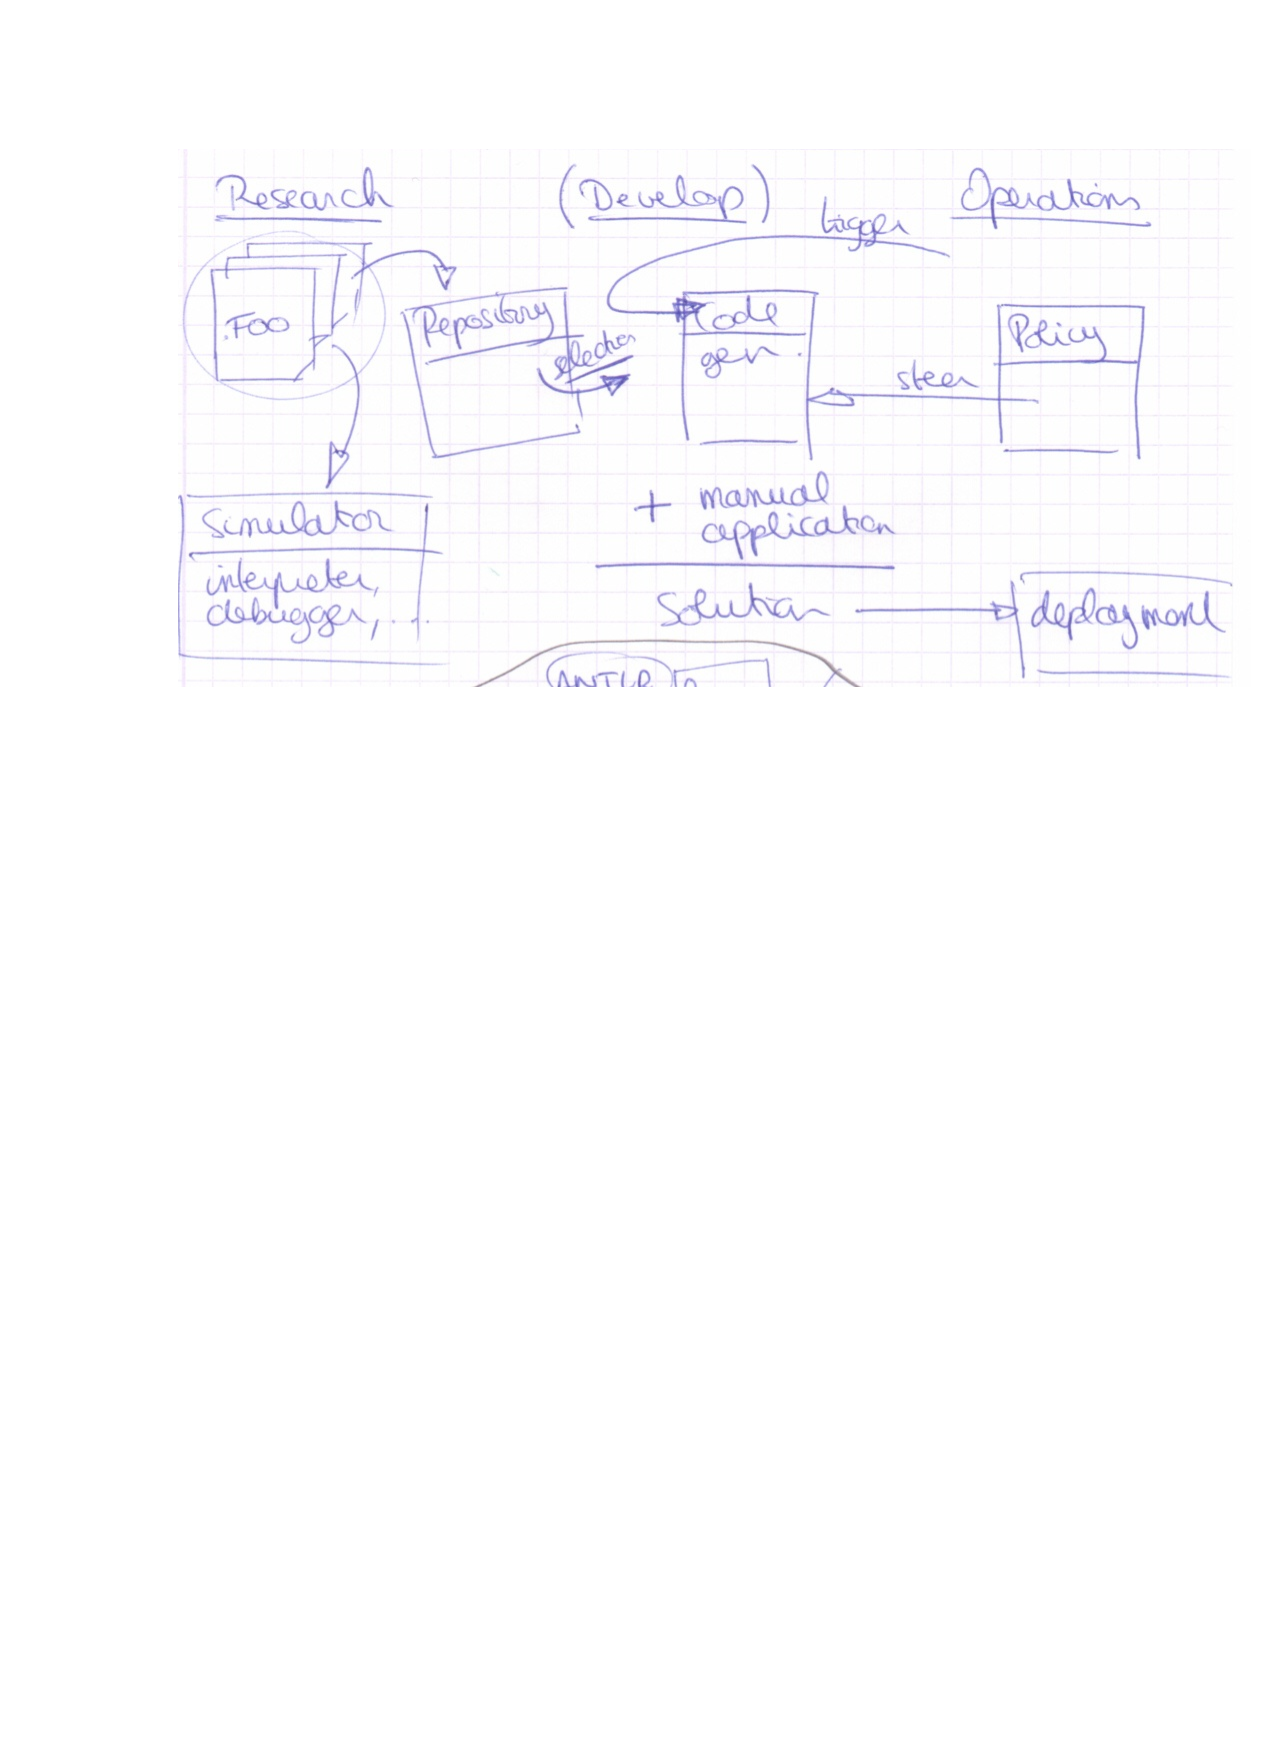
\includegraphics[width=\linewidth]{resources/arch-functional.pdf}
  \caption{Functionele architectuur}
  \label{fig:arch-functional}
\end{figure}

\subsection{FOO-lang}
\label{subsection:arch-foo-lang}

De eerste belangrijke component van de oplossing is de domeinspecifieke taal,
waarmee detectiealgoritmes kunnen beschreven worden. De belangrijkste
doelstelling van de taal is om de functionaliteit zo optimaal mogelijk te
organiseren. Hierdoor wordt getracht om het gebruik van de \mcu en het gebruik
van de draadloze radio te beperken. Deze doelstelling wordt ook weerspiegeld in
de naam: Functie Organisatie Optimalisatie (Engels: Function Organisation
Optimisation), kortweg: FOO-lang.

De belangrijkste doelgroep wat betreft gebruikers, zijn onderzoekers van IDS in
WSN. Met FOO-lang kunnen zij beschikken over een formele taal om
inbraakdetectiealgoritmes voor WSN te beschrijven.

Het is van primordiaal belang dat de taal zo dicht mogelijk aansluit bij
bestaande kennis en vertrouwde paradigma. Daarom wordt voorgesteld om dicht bij
de C programmeertaal aan te blijven leunen en deze uit te breiden met niet
ongewone constructies om het niveau van de taal op een hoger niveau van
abstractie te brengen. Dit hogere niveau sluit meer aan bij een functionele en
platform-onafhankelijke beschrijving.

Om de doelstelling na te streven is het belangrijk dat er control is over de
iteratieve aspecten van de algoritmen. Deze gaan typisch om de sensorknopen in
de nabijheid van de knoop in kwestie. Door de functionaliteit van het domein te
centraliseren rond deze knopen, is het mogelijk om deze iteraties weg te
werken. Door het defini\"eren van gebeurtenissen waarop kan gereageerd worden
met functionaliteit, is het mogelijk om abstractie te maken van de volledige
lijst van sensorknopen en het algoritme in stukken te breken die als reacties
op de gebeurtenissen kunnen beschreven worden.

Om het functionele karakter verder te onderstrepen is het belangrijk dat zoveel
mogelijk technische aspecten uit de algoritmen geweerd worden. Een typische
voorbeeld is de typering van variabelen. Typering zal een noodzaak blijken,
maar moet op zijn minst optioneel zijn en indien nodig voorzien worden als een
beperkte set van functionele types. Dit is ook een belangrijke voorwaarde voor
de platform-onafhankelijkheid.

\subsection{Centrale opslagplaats}
\label{subsection:arch-repository}

Al deze platform-onafhankelijke en formele beschrijvingen van
detectiealgoritmen, kunnen vervolgens samengebracht worden in een centrale
opslagplaats. Het hoeft geen betoog dat hiervoor een website kan voorzien
worden, die als portaal kan dienen. Een heel aantal klassieke voorzieningen
kunnen hierbij getroffen worden: zoekmogelijkheden, gebruiksstatistieken,
commentaar, samenwerkmogelijkheden \dots

Allerhande integraties kunnen voorzien worden om op transparante wijze met
zoveel mogelijk de facto standaard diensten te kunnen samenwerken. Hierbij
denken we aan diensten die opslag van programmacode aanbieden, of meer algemeen
opslag van bestanden, tot processturingsplatformen of probleemopvolgsystemen.

De toegang tot de broncode van de algoritmen moet enerzijds mogelijk zijn via
de visuele website, maar moet zeker geautomatiseerd ge\"integreerd kunnen
worden, zodat bv. compilatieprocessen de laatste versie van een algoritme
kunnen downloaden zonder tussenkomst van een persoon.

\subsection{Code generator}
\label{subsection:arch-codegen}

Het kloppend hart van de oplossing bestaat uit de code generator. Deze
accepteert de in FOO-lang geschreven algoritmes en vormt deze om tot
georganiseerde code voor het geselecteerde platform, eventueel voor een gegeven
taal \dots

De generator moet de doelstellingen van de oplossinsstrategie implementeren en
de resulterende code op zo'n manier structureren dat deze minder impact heeft
op de werking van de sensorknoop.

Om een volledig geautomatiseerde werking toe te laten is het belangrijk dat de
aansturing van de generator in zo'n een context mogelijk is. De configuratie
van de generator moet via een bestand of aan de hand van oproepparameters
gespecificeerd kunnen worden, zonder verdere menselijke tussenkomst.

\subsection{Uitbatingsbeleid}
\label{subsection:arch-policy}

Een volledig geautomatiseerde oplossing laat toe om een uitbatingsbeleid te
introduceren op veel fijnere schaal. Het wordt immers mogelijk om zelfs per
sensorknoop een ``persoonlijk'' configuratie te gaan onderhouden, bouwen en te
verspreiden.

Hierbij komt de oplossing ook te gemoed aan bv. de nood van sommige algoritmes
om op verschillende soorten knopen verschillende functionaliteit te voorzien.
Maar vanuit een uitbatingsbeleid is dit een groot voordeel. Naast de
optimalisatie van het gebruik van de middelen van \'e\'en knoop, kan nu ook een
spreiding over verschillende knopen helpen om het gemiddeld aantal algoritmen
per knoop te verlagen en zelfs dynamisch op regelmatige tijdstippen te wijzigen.

Indien gecombineerd met voorzieningen die OTAP toelaten, kan het
gedistribueerde IDS op elk ogenblik gewijzigd worden. Tal van mogelijkheden
ontstaan zo.

\subsection{Ontwikkeling en integratie}
\label{subsection:arch-integration}

Naast het IDS is er natuurlijk nog de eigenlijke toepassing die op de
sensorknoop zal ge\"installeerd en uitgebaat worden. Ook deze moet optimaal
verwerkt kunnen worden in het samenstellingsproces.

De minimale vereisten zijn dat het generatieproces duidelijke markeringen in de
resulterende code achterlaat, zodat de integratie met de toepassinscode
mogelijk is. Deze markeringen kunnen ook voorzien worden in de vorm van
invoegdirectieven die tijdens het compilatieproces bijkomende bestanden kan
opnemen zonder verdere tussenkomst van een ontwikkelaar.

\subsection{Verdere opportuniteiten}
\label{subsection:arch-opportunities}

Met een centrale opslagplaats en een volledige automatiseerbare code generatie
en compilatieproces, zijn tal van ondersteunende toepassingen denkbaar.

Een voorbeeld dat van groot belang kan zijn voor onderzoekers is een
gestandaardiseerde simulatieomgeving. Deze zou kunnen opgebouwd worden met de
code generator, voorzien van een implementatie voor een virtueel platform, die
bruikbare code genereert voor de simulatieomgeving. Een integratie zou kunnen
bestaan in een implementatie in Javascript, wat toelaat om de simulatie toe te
voegen aan de centrale opslagplaats en dynamisch verschillende combinaties van
algoritmen uit de centrale opslagplaats te testen voor ze te integreren in een
echte omgeving.

\subsection{Scope}
\label{subsection:arch-scope}

De voorgaande hoogniveau functionele analyse toont vooral aan dat met de
basiscomponenten veel andere opportuniteiten in bereik liggen. Het is
belangrijk om deze opportuniteiten in het vizier te houden, zodat er geen
uitgesloten worden door de implementatie.

De minimale set aan basiscomponenten zal ook in deze thesis verder uitgewerkt
worden aan de hand van een prototype. Het betreft de code generator met
ondersteuning voor een eerste platform en programmeertaal combinatie.

\section{Technische architectuur}
\label{section:arch-technical}

Figuur \ref{fig:arch-technical} toont de vertaling van de beoogde functionele
scope naar meer technische componenten. 

\begin{figure}[ht]
  \centering
  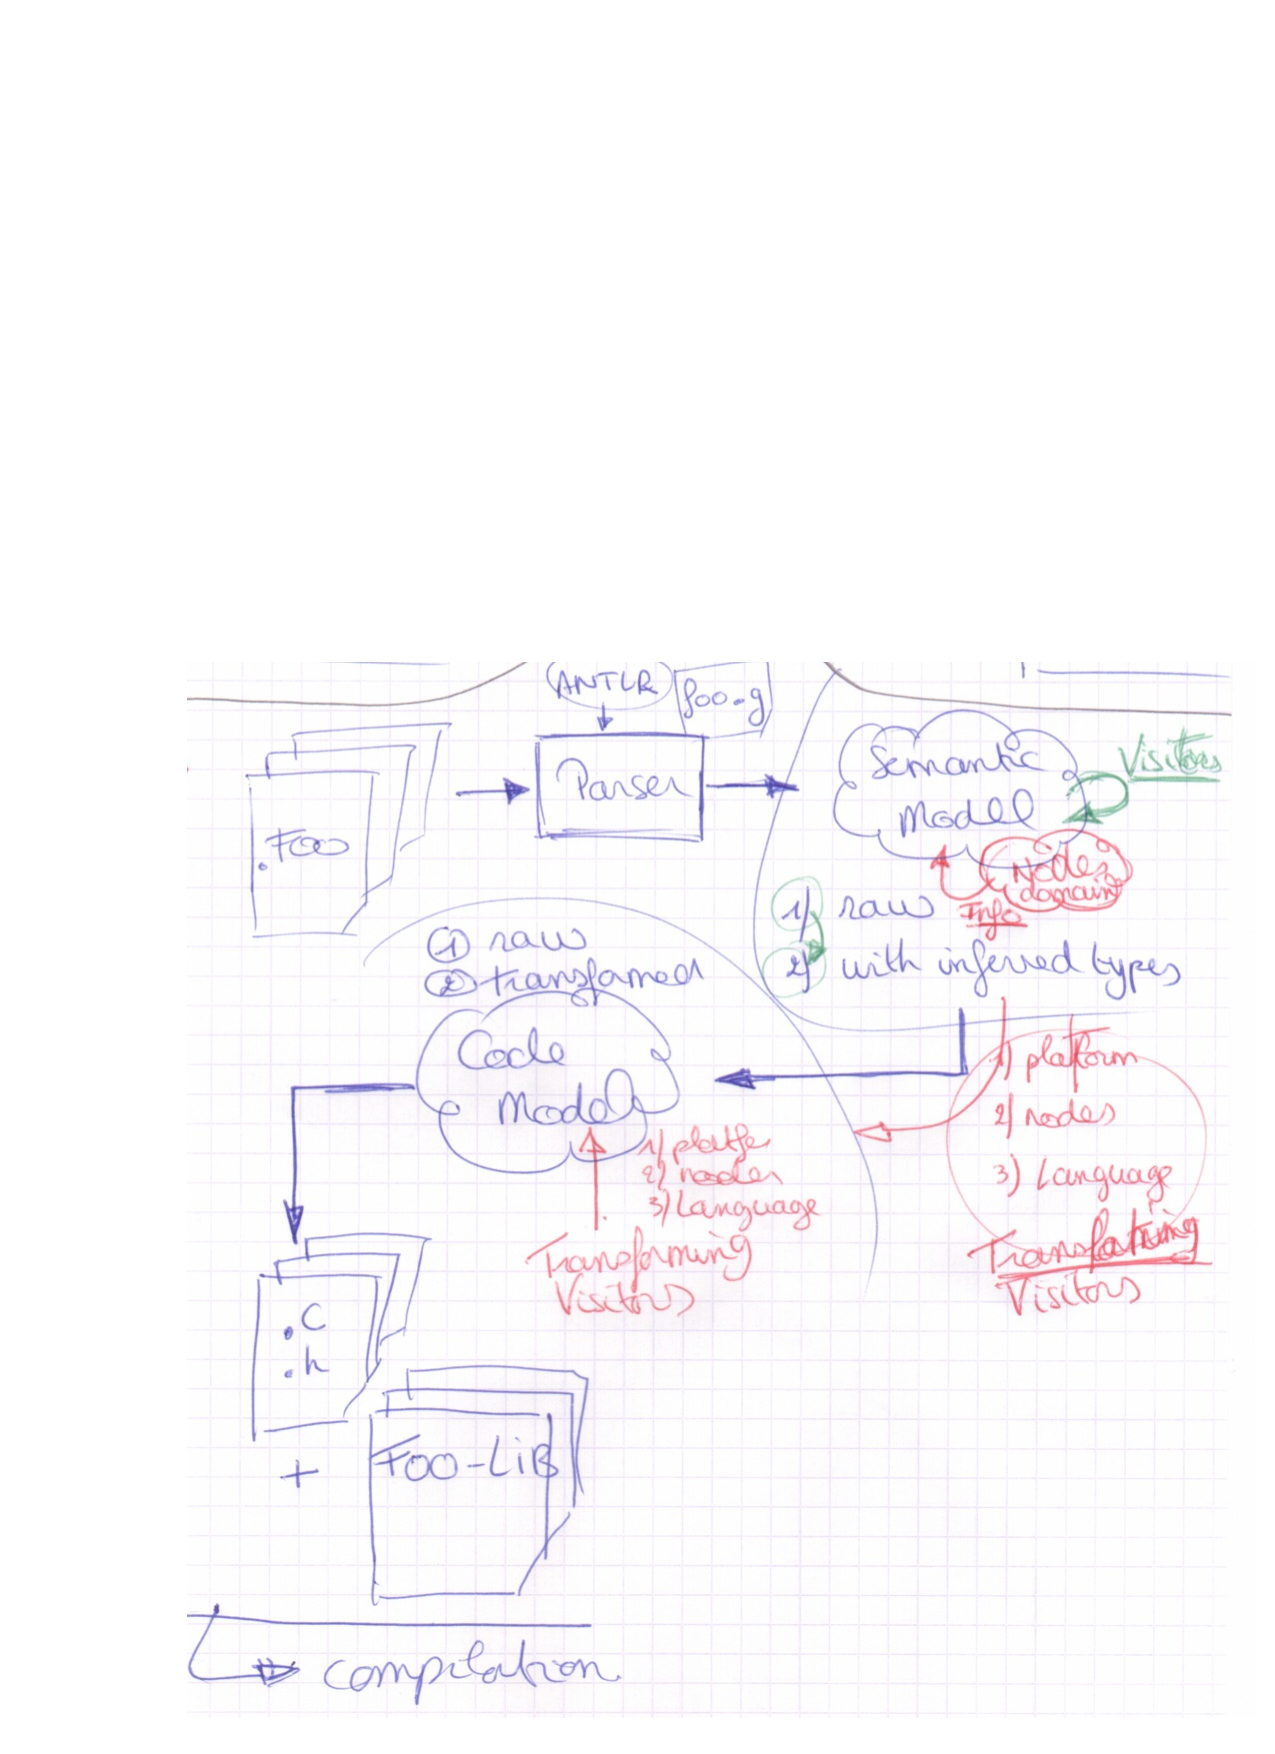
\includegraphics[width=0.7\linewidth]{resources/arch-technical.pdf}
  \caption{Technische architectuur}
  \label{fig:arch-technical}
\end{figure}

De verwerking verloopt als volgt: een parser analyseert de FOO-lang broncode en
produceert een zgn. abstracte syntax boomvoorstelling (Engels: \emph{Abstract
Syntax Tree} (AST). Deze AST wordt vervolgens ingeladen in een semantisch model
(SM) \citep{fowler2010domain}. Door middel van verschillende transformaties
wordt dit SM model vervolledigd (bv. type deductie) en vervolgens omgezet in
een code model (CM). Ook dit CM zal opnieuw door middel van verschillende
transformaties omgezet worden in een structuur die te vergelijken is met een
AST en toelaat om rechtstreeks omgezet te worden in programmacode.

\subsection{Semantisch model}
\label{subsection:arch-semantic-model}

Een semantisch model bevat de volledige semantisch correcte voorstelling van de
boogde functionaliteit. In die optiek vertoont het sterke overeenkomsten met
een klassiek domein model \citep{fowler2010domain}. Omdat dit laatste echter
veel rijker is aan functionaliteit en een semantisch model typisch meer
informatie-geori\"enteerd is, wordt er een onderscheid gemaakt in de naamgeving.

Het model is volledig ge\"ent op het domein waarvoor het opgebouwd wordt. In
figuur \ref{fig:arch-semantic-model} is een sterk vereenvoudigde voorstelling
van het SM voor het inbraakdetectie domein weergegeven. Het bevat alle
functionele aspecten die nodig geacht worden om het domein functioneel te
beschrijven.

\begin{figure}[ht]
  \centering
  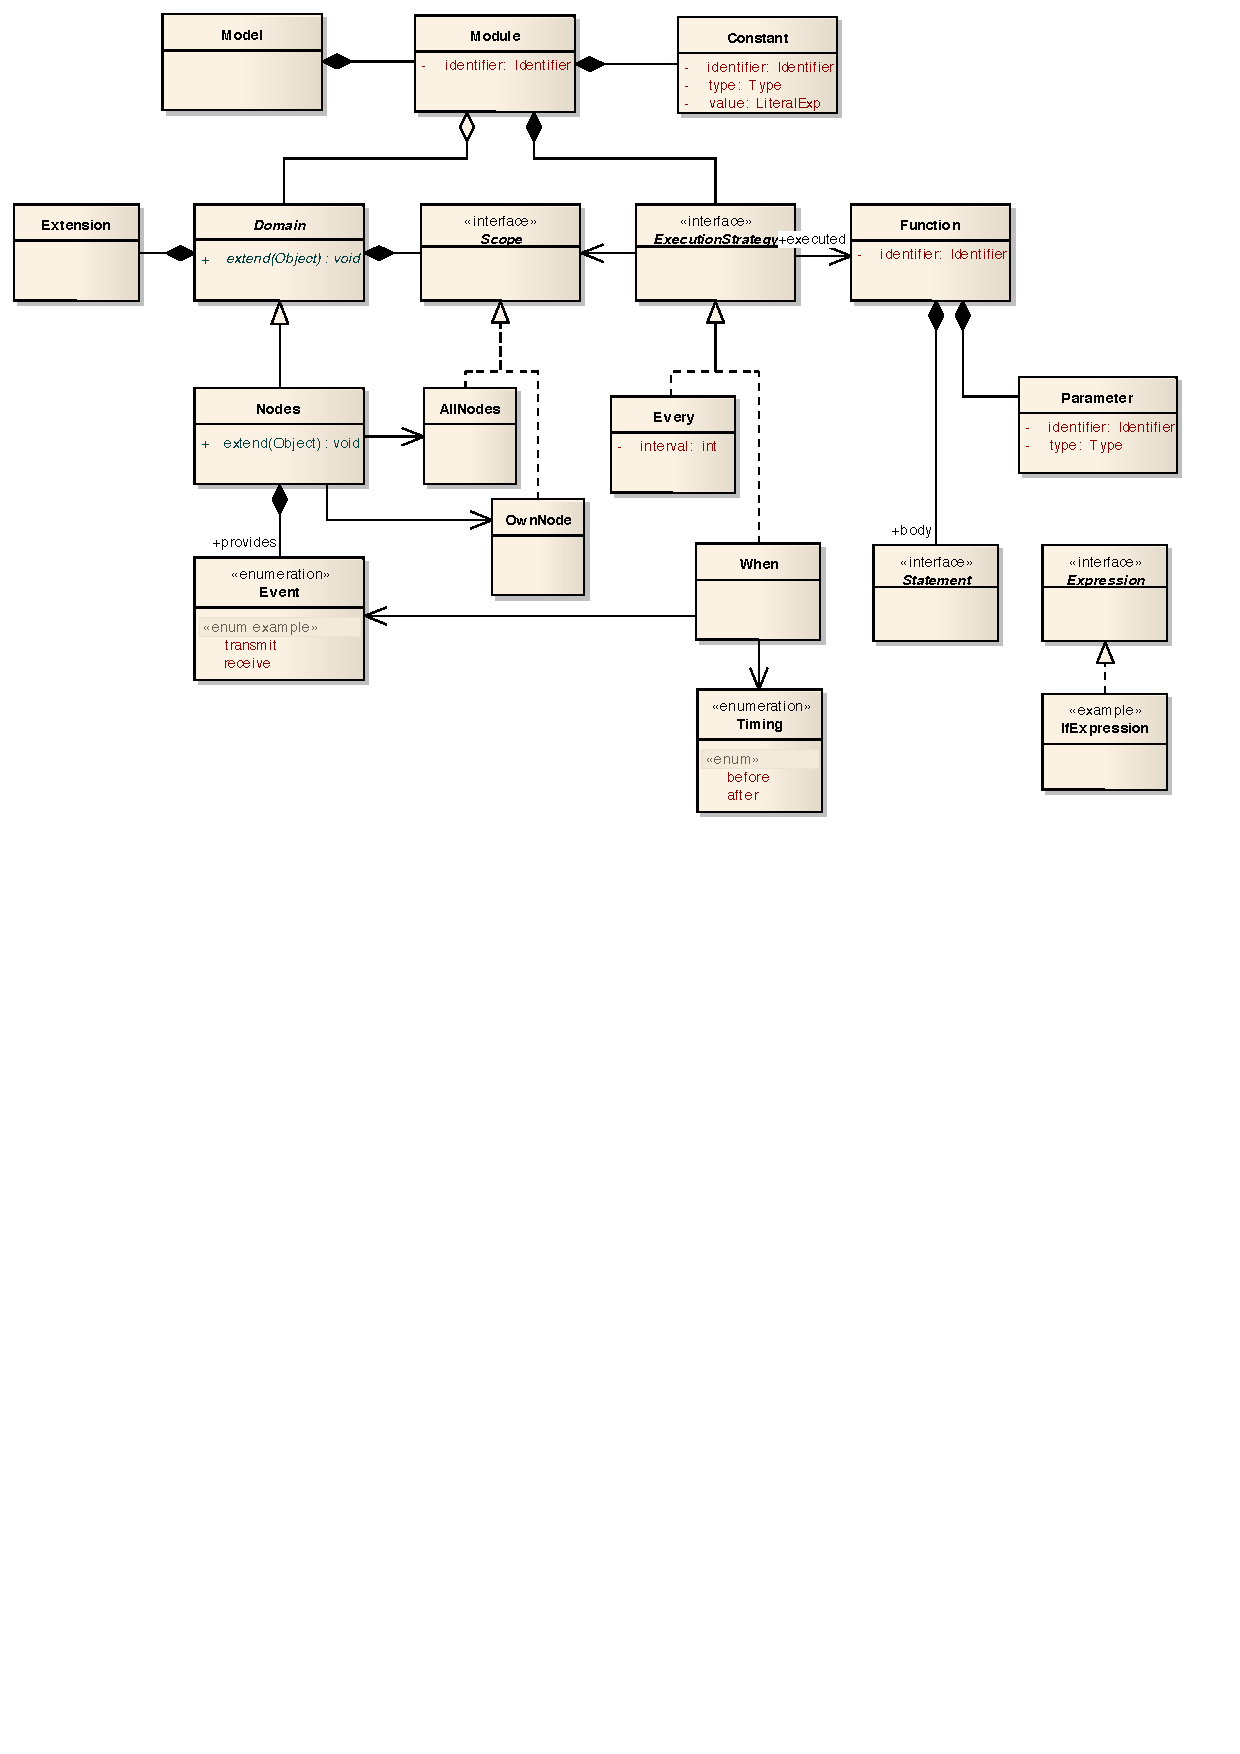
\includegraphics[angle=90,width=0.865\linewidth]{resources/semantic.pdf}
  \caption{Semantisch model}
  \label{fig:arch-semantic-model}
\end{figure}

Op het hoogste niveau herkennen we het model als alles omvattende entiteit.
Hieronder worden de modules geplaatst, die overeenkomen met telkens \'e\'en
algoritme. Modules bevatten functionaliteit in de vorm van
functiebeschrijvingen.

Het centrale concept is dat van de uitvoeringsstrategie (Engels:
\emph{Execution Strategy})\footnote{Er is geopteerd om in de programmacode van
de generator een Engelstalige terminologie aan te houden.}. Deze verbindt
functionaliteit met de knopen. Verschillende soorten strategie\"en zijn
voorzien: een reactie op een gebeurtenis (\emph{Handler}) en een weerkerende
actie (\emph{Every}).

Op een lager niveau wordt de functionaliteit beschreven aan de hand van een
syntax die nauw aansluit bij deze van de C programmeertaal. Deze is echter wel
uitgebreid met constructies van een hoger abstractieniveau, om op een
functionelere manier om te kunnen gaan met de entiteiten uit het domein.

\subsection{Code model}
\label{subsection:arch-code-model}

Via verschillende transformaties, wordt het SM omgezet in een CM. Deze overstap
vertaalt in essentie de functionele concepten naar overeenkomstige patronen in
een semantiek die direct aanleunt bij programmeertalen.

Het code model voorziet een hi\"erarchie van een compilatie unit, met daaronder
modules en binnen elke module secties. Dit is een abstracte voorstelling van
respectievelijk de gehele compilatie, de functionele modules en de bestanden
waaruit die modules opgebouwd zullen worden. In termen van de C programmeertaal
is dit het geheel van C en aanverwante bestanden, het concept van een C module
en op het laagste niveau de effectieve C en hoofding bestanden.

Een sectie bestaat dan uit \'e\'en of meerdere code constructies: functie
declaraties, expressies, statements \dots Deze code constructies zijn rijker
dan bv. de C programmeertaal. Het zal de taak zijn van opeenvolgende
transformaties om deze niet-gekende constructies voor een bepaald platform
en/of programmeertaal om te vormen naar wel ondersteunde constructies.


%!TEX root=masterproef.tex

\chapter{Implementatie}
\label{chapter:implementatie}

Voor deze thesis werd een prototype ge\"implementeerd van de generator. Hierbij
werd FOO-lang gedefinieerd tot op het niveau dat het mogelijk was om twee
realistische voorbeelden te beschrijven. Ook de generator werd uitgewerkt tot
het niveau dat het mogelijk was om de twee voorbeelden te genereren. Zowel de
voorbeelden als de implementatie van de taal en generator zijn zo uitgewerkt
dat ze als realistische referentie kunnen dienen en dat de resultaten het
potentieel waarborgen.

Het hoofdstuk wordt ingeleid met een korte sectie, \ref{section:devel-python},
over Python, de programmeertaal die werd gekozen voor de implementatie van het
prototype.

Daarna wordt FOO-lang in meer detail bekeken in sectie
\ref{section:devel-foo-lang}. Aan de hand van voorbeelden en de grammatica
introduceren we de taal, de mogelijkheden die ze biedt alsook de beperkingen
die ze introduceert. Een elementair voorbeeld wordt vervolgens als rode draad
doorheen het hoofdstuk gebruikt om de volledige generatie van FOO-lang
beschrijving tot C programmacode te illustreren aan de hand van een effectief
voorbeeld.

Sectie \ref{section:devel-codegen} belicht de generator met in hoofdzaak de
tweeledige taxonomie van het SM en het CM. De verschillende transformaties die
uitgevoerd worden op beide modellen worden kort samengevat en het onderliggende
implementatie van het \emph{visitor} patroon \citep{gamma1994design} wordt
toegelicht.

De generator wordt vergezeld van gemeenschappelijke basisfunctionaliteit in de
vorm een softwarebibliotheek, genaamd FOO-lib. Sectie
\ref{section:devel-foo-lib} overloopt kort de verschillende modules en kadert
het geheel in de context van de generator en de taal.

\section{Python}
\label{section:devel-python}

Als programmeertaal voor het prototype werd geopteerd voor Python. Python is
een ge\"interpreteerde taal met dynamische typering die verschillende
programmeerparadigma ondersteunt: imperatief, object-geori\"enteerd en
functioneel. Dit maakt het een zeer veelzijdige taal die veel mogelijkheden
biedt.

Python is ook volledig open in zijn structuur. Alles is toegankelijk en niets
wordt verborgen. Dit laat toe om elk aspect van een gegevensstructuur of object
te manipuleren. Dit kan heel handig zijn, maar kan ook leiden tot onverwachte
neveneffecten.

Alle functionaliteit, klassen of gewone functies, worden verzameld in een
\emph{module} en andere modules kunnen vervolgens deze functionaliteit
importeren. Door de volledige transparantie en dankzij ver doorgedreven
mogelijkheden tot introspectie, kan de implementatie van een module dynamisch
aangepast worden. Dit werd o.a. uitvoerig toegepast voor het implementeren van
het \emph{visitor} patroon, verder besproken in sectie
\ref{subsubsection:devel-visitor-pattern}.

Ofschoon mijn ervaring met Python beperkt was, is Python zeker geen slechte
keuze voor de implementatie van deze software. Zo beschikt de taal over een
zeer rijke verzameling van kant-en-klare modules, die toelaten om enkele
basistaken snel te implementeren. De flexibiliteit en de mix van zowel
imperatief als object-geori\"enteerd als functioneel programmeren liet
meermaals toe om bepaalde zaken op creatieve manier te implementeren.

Het feit dat in essentie een nieuwe taal was, bracht ook een bijkomende
leercurve met zich mee. Ook zorgde voortschrijdend inzicht voor stapsgewijze
verbeteringen aan bepaalde constructies, die echter soms door tijdbeperkingen
niet voor alle overige code konden bijgewerkt worden.

\section{FOO-lang}
\label{section:devel-foo-lang}

Maar de echte belangrijke taal in dit geval is niet Python, maar FOO-lang.
Codevoorbeeld \ref{lst:hello.foo} toont de implementatie van een elementair voorbeeld
in FOO-lang. Aan de hand van dit voorbeeld introduceren we nu de typische
bouwstenen van FOO-lang en doorlopen we het hele generatieproces.

\inputminted[linenos,frame=lines,framesep=2mm,fontsize=\footnotesize]{js}{../src/foo-lang/examples/hello.foo}
\vspace{-5mm}
\captionof{listing}{Elementair voorbeeld in FOO-lang: \ttt{hello.foo}
  \label{lst:hello.foo}}
\vspace{3mm}

De code start op regel 6 met de declaratie van een \emph{module}. Een module is
een op zich staand geheel en zou bv. een detectiealgoritme kunnen zijn. Alles
wat volgt op de declaratie van de module, maakt er deel van uit.

Op regel 8 introduceren we een \emph{const}ante, \ttt{interval} en stellen die
gelijk aan \ttt{1000}. Hier zien we een eerste voorbeeld van het ontbreken van
expliciete typering in FOO-lang. Dankzij type deductie zal in dit geval het
type van \ttt{interval} overeenkomen met een \emph{IntegerType}, omdat de
waarde \ttt{1000} gevormd is als een integer getal.

Ofschoon FOO-lang ge\"introduceerd wordt als DSL voor inbraakdetectie in DSN,
specificeert het zijn domein als dat van \emph{sensorknopen} of \emph{nodes}.
Algoritmes met betrekking tot inbraakdetectie in DSN, hebben \'e\'en belangrijk
gemeenschappelijke entiteit en dat zijn de sensorknopen. Deze communiceren met
elkaar en op basis van die communicatie zijn zowat alle algoritmes opgebouwd.

Het concept van een knoop of \emph{node} wordt beheert door het raamwerk dat
opgebouwd wordt door de generator. De algoritmes krijgen toegang tot deze
knopen via een aantal functionele constructies. Maar ze kunnen de
basisdefinitie van een knoop in het domein uitbreiden met hun eigen
eigenschappen. Dit gebeurt bv. op regel 10, waar (de knoop van) het domein
uitgebreid wordt met een eigenschap \ttt{sequence}. Deze eigenschap wordt
expliciet getypeerd met het \emph{byte} type en krijgt als initi\"ele waarde
\ttt{0}.

FOO-lang is een \emph{functie}-geori\"enteerde taal die tracht om de functies
in de verschillende modules, zo te organiseren dat de uitvoering ervan de \mcu
of de draadloze radio zo min mogelijk belast. Op regel 14 wordt een functie
gedefinieerd, genaamd \ttt{step}. Ze accepteert \'e\'en parameter, genaamd
\ttt{node}. We merken opnieuw op dat deze parameter niet getypeerd is.

De inhoud van de functie bestaat uit programmeerconstructies die niet ongewoon
zullen overkomen en feitelijk bijna gewone C code zou kunnen zijn. Een
conditie, een eigenschap, een waardeverhoging,\dots We zien hier onze eerder
toegevoegde eigenschap, \ttt{sequence}, terug opduiken.

Regel 20 brengt alle voorgaande definities nu samen in een
\emph{uitvoeringsstrategie}. FOO-lang tracht doormiddel van zijn syntax ook te
lezen als een natuurlijk taal. Indien we regel 20 gewoon lezen, zou dit iets
kunnen opleveren als ``\emph{At every (passing of) interval with nodes do (the
function named) step.}''. En dat is exact wat deze regel definieert.

In deze ene regel zien we de klassieke lus over alle gekende knopen die in
zowat alle algoritmen wel in \'e\'en of andere vorm terugkomt, echter nu is de
lus geabstraheerd tot zijn functionele betekenis.

\subsection{Syntax en grammatica}
\label{subsection:devel-foo-lang-grammar}

Het voorgaande voorbeeld gebruikt slechts een kleine subset van de volledige
mogelijkheden van FOO-lang. De volledige grammatica van FOO-lang, zoals
gedefinieerd in het kader van dit prototype, is opgenomen in appendix
\ref{appendix:foo-lang-grammar}. Deze appendix bevat de \emph{Extended
Backus-Naur Form} (EBNF) die de taal eenduidig bepaalt, alsook een visualisatie
van de verschillende regels.

We bespreken hier kort enkele constructies die nog niet eerder voorkwamen.

\subsubsection{Importeren van functionaliteit}

Het is mogelijk om externe functies te importeren. Dit gebeurt aan de hand van
de constructie \ttt{from ... import ... }. Hiermee wordt een functie
ge\"importeerd vanuit een module. Zo'n module kan een andere FOO-lang module
zijn, of een extern gedefinieerde functie uit een softwarebibliotheek. In
\ref{section:devel-foo-lib} introduceren we de FOO-lib, de standaard
softwarebibliotheek die de code generatie vervolledigd. Hieruit worden typisch
functies geraadpleegd in de meeste beschrijvingen.

\subsubsection{Reageren op gebeurtenissen}

Naast het herhaaldelijk uitvoeren van een functie is het ook mogelijk om een
functie te koppelen aan een gebeurtenis in de context van het domein en de
knopen. In plaats van de \ttt{with ... do} constructie is het ook mogelijk om
een voor of na (\ttt{before} en \ttt{after}) de uitvoering van een functie
binnen het kader van het domein, een functie uit te voeren. Codevoorbeeld
\ref{lst:foo-event_handler} geeft een eenvoudig voorbeeld waarbij we ontvangen
berichten tellen als deze aan ons geadresseerd waren.

\begin{listing}[ht]
  \begin{minted}[linenos,frame=lines,framesep=2mm,fontsize=\footnotesize]{javascript}
after nodes receive do function(me, sender, from, hop, to, payload) {
  if(to == me) {
    me.msg_count++
  }
}
  \end{minted}
  \vspace{-5mm}
  \caption{Voorbeeld van het reageren op een gebeurtenis}
  \label{lst:foo-event_handler}
\end{listing}

In dit voorbeeld merken we ook op dat functies anoniem kunnen gedefinieerd
worden en niet eerst met een naam gedefinieerd worden.

\subsubsection{Verschillende situaties afhandelen}

Het \ttt{case statement} laat toe om eenzelfde expressie te evalueren in
verschillende situaties. Typisch gebruik voor deze constructie is het
analyseren van ontvangen gegevens. Codevoorbeeld \ref{lst:foo-case} illustreert dit.

\begin{listing}[ht]
  \begin{minted}[linenos,frame=lines,framesep=2mm,fontsize=\footnotesize]{javascript}
after nodes receive do function(me, sender, from, hop, to, payload) {
  case payload {
    contains([#marker1, value]) {
      sender.msg_sent1++
    }
    contains([#marker2, value]) {
      sender.msg_sent2++
    }
    else {
      sender.msg_other++
    }
  }
}
  \end{minted}
  \vspace{-5mm}
  \caption{Voorbeeld van het afhandelen van verschillende situaties}
  \label{lst:foo-case}
\end{listing}

In dit voorbeeld wordt de ontvangen berichten geanalyseerd en gecatalogeerd op
basis van de inhoud. Als in een berichte \ttt{\#marker1} wordt gevonden wordt
\ttt{msg\_sent1} verhoogd, in het geval van \ttt{\#marker2}, \ttt{msg\_sent2}
en anders \ttt{msg\_other}.

Deze constructie is in feite een mooiere syntax voor een overeenkomstige
constructie op basis van \ttt{if statements}, zoals weergegeven in listing
\ref{lst:foo-case-if}.

\begin{listing}[ht]
  \begin{minted}[linenos,frame=lines,framesep=2mm,fontsize=\footnotesize]{javascript}
after nodes receive do function(me, sender, from, hop, to, payload) {
  if payload.contains([#marker1, value]) {
    sender.msg_sent1++
  } else if payload.contains([#marker2, value]) {
    sender.msg_sent2++
  } else {
    sender.msg_other++
  }
}
  \end{minted}
  \vspace{-5mm}
  \caption{Alternatieve constructie voor verschillende situaties}
  \label{lst:foo-case-if}
\end{listing}

Dit voorbeeld introduceert tevens nog drie andere belangrijke constructies: het
\emph{atom}, lijsten en patroon koppeling.

\subsubsection{Atomen}

\emph{Atomen} werden ontleed aan Erlang. Ze stellen een uniek herkenbare
entiteit voor. Het is aan de generator met hulp van het platform en/of domein
en/of doeltaal om hiervoor een geschikte voorstelling te vinden.

In het geval van dit prototype werden twee bytes voorzien om een unieke
identificatie te maken van delen in berichten. De generator kan hier
verschillende strategie\"en volgen en beslissen op basis van de verschillende
\emph{atoms} die hij tegenkomt.

\subsubsection{Lijsten}

Lijsten worden voor verschillende doeleinden gebruikt. Ze worden syntactisch
gespecificeerd door middel van vierkante haken. Zo worden ze meestal al een
letterlijke voorstelling van de lijst opgenomen. In het voorbeeld in listing
\ref{lst:foo-case} is de \ttt{payload} parameter zo'n lijst. Ook het argument
van de \ttt{contains} methode die toegepast wordt op \ttt{payload} is een
lijst. De parameter verwacht echter niet echt een lijst, maar een patroon. In
dit geval is de lijst een deel van het patroon.

\subsubsection{Patroon koppeling}

Door middel van patronen kan er een kopping gemaakt worden tussen gegevens. In
het voorbeeld in codevoorbeeld \ref{lst:foo-case} accepteert de \ttt{contains}
methode op een \emph{lijst} een patroon. Dit patroon is een lijst en bestaat
uit variabele en niet-variabele elementen. De \ttt{contains} methode zal
trachten de niet-variabele elementen herkennen in de lijst en vervolgens bij
een succesvolle herkenning een kopping te maken tussen de variabele elementen
en de waarden in de oorspronkelijke lijst.

\subsubsection{Complexe types}

In codevoorbeeld \ref{lst:hello.foo} zagen we reeds kort een voorbeeld van typering.
De \ttt{sequence} eigenschap werd getypeerd als een \ttt{byte}. Naast
\ttt{byte} zijn er ook nog \ttt{integer}, \ttt{float}, \ttt{boolean} en
\ttt{timestamp} als standaard eenvoudige types.

Vergelijkbaar met lijsten is er ook het \emph{tuple} type. Dit zijn lijsten van
types en defini\"eren de types van de elementen van een lijst van vaste lengte.

Van alle types kan ook een veelvoud gedefinieerd worden door het toevoegen van
een \ttt{*} achter het type. Zo kunnen lijsten van een bepaald type
gedefinieerd worden. Gecombineerd met het \emph{tuple} type, ontstaat zo bv. de
mogelijkheid om lijsten van \emph{records} te defini\"eren.

In codevoorbeeld \ref{lst:foo-complex_type} wordt het \ttt{nodes} domein uitgebreid
met een \ttt{inbox} eigenschap. Deze bestaat uit meerdere \emph{tuples} die op
hun beurt bestaan uit een \ttt{timestamp} en meerdere \ttt{bytes}.

\begin{listing}[ht]
  \begin{minted}[linenos,frame=lines,framesep=2mm,fontsize=\footnotesize]{javascript}
extend nodes with {
  inbox : [timestamp, byte*]* = []
}
  \end{minted}
  \vspace{-5mm}
  \caption{Voorbeeld van een complex type}
  \label{lst:foo-complex_type}
\end{listing}

\subsubsection{Strings}

Grote afwezige in deze versie van FOO-lang zijn strings. Dit lijkt initieel
contra-intu\"itief, maar bij nader inzien zijn strings niet echt van toepassing
in het domein van inbraakdetectie in DSN. De introductie van strings in
FOO-lang zou op dit ogenblik tevens een herschrijven van de grammatica vragen.

\section{Code generator}
\label{section:devel-codegen}

Met FOO-lang zijn we nu in staat om inbraaddetectiealgoritmes te beschrijven.
Deze FOO-lang code moet vervolgens door de code generator omgezet worden in een
gewone programmeertaal. In het geval van dit prototype is dat C.

\subsection{Opbouw}

Figuur \ref{fig:devel-component-overview} geeft een overzicht van de opbouw van
de oplossing.

\begin{figure}[ht]
  \centering
  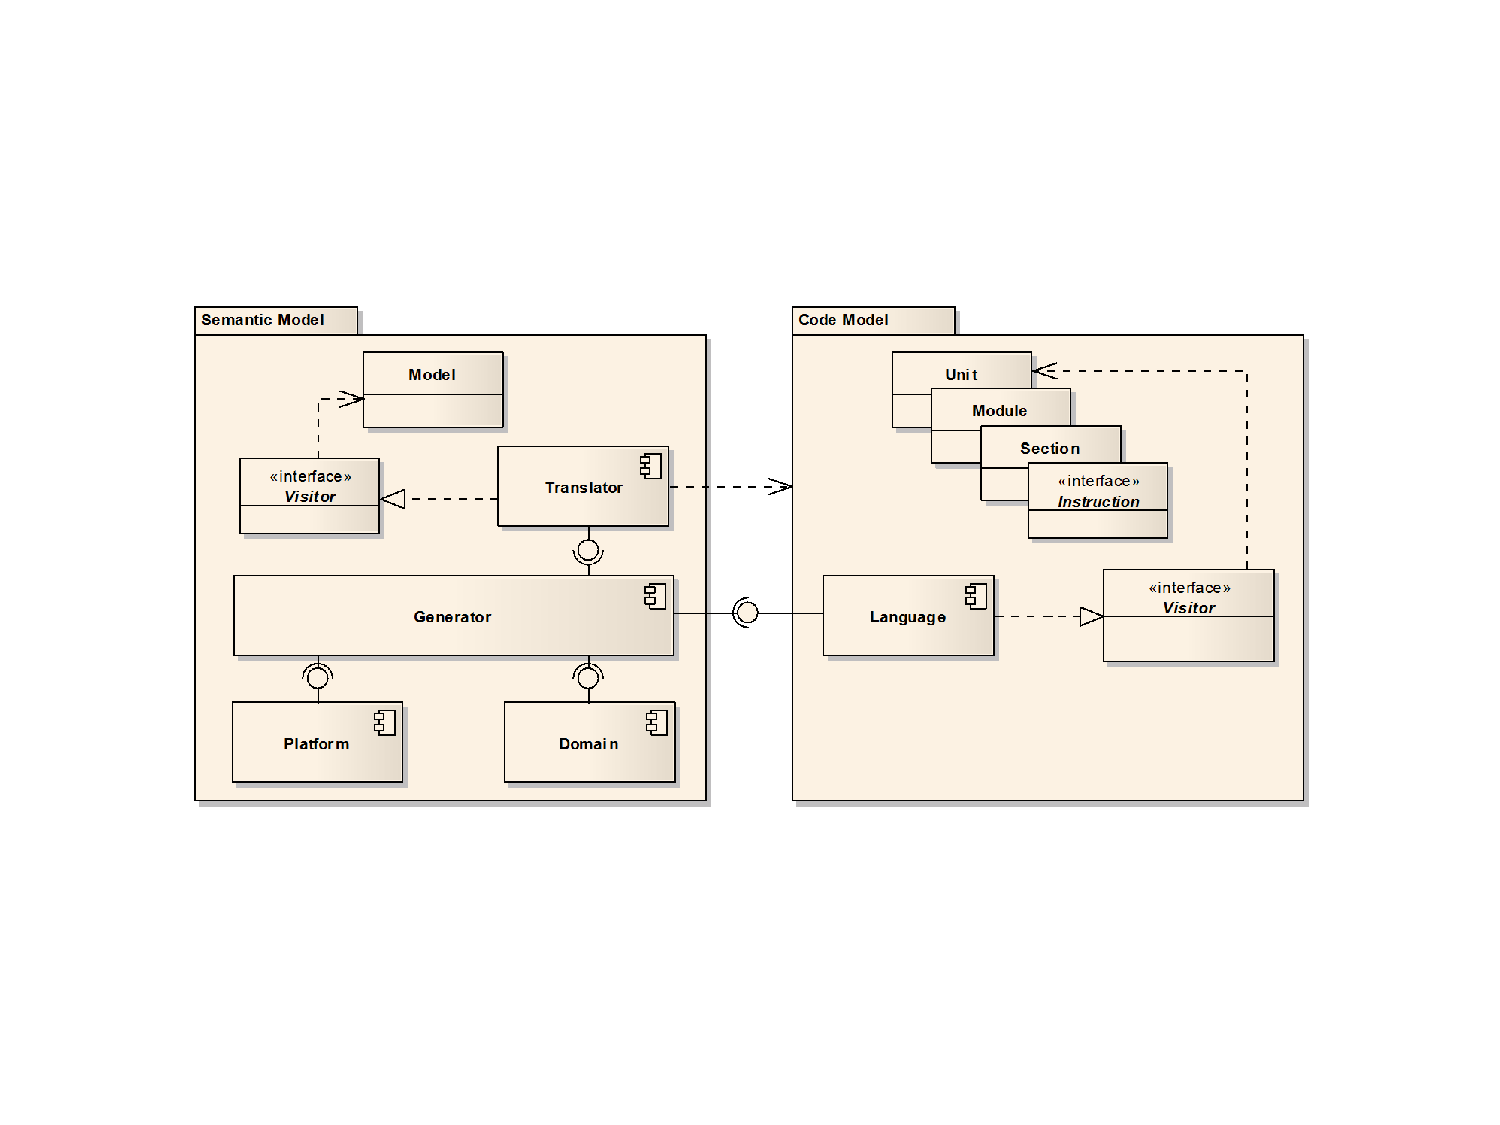
\includegraphics[width=\linewidth]{resources/component-overview.pdf}
  \caption{Overzicht van componenten en kernentiteiten}
  \label{fig:devel-component-overview}
\end{figure}

Intern bestaat de hele oplossing uit twee grote delen: het semantische en het
code gedeelte. Binnen het semantische gedeelte vinden we het SM terug. Dit
model kan benaderd worden door middel van een zgn. \emph{visitor}, een
implementatie van het \emph{visitor pattern}. Aan de hand van deze
\emph{visitor} kunnen transformaties van het model gerealiseerd worden.

Het SM is de primaire invoer voor de generator. Die kan zijn werk slechts
vervullen door middel van een compositie met \emph{platform-} en
\emph{domeininformatie}, een vertaler (Engels: \emph{Translator}) die elementen
uit het semantische gedeelte kan omzetten naar overeenkomstige elementen in het
code gedeelte en de uiteindelijk beoogde programmeertaal (Engels:
\emph{Language}).

De programmeertaal maakt deel uit van het CM. Dit is op zijn beurt opgebouwd
uit een hi\"erarchie van vier niveaus. De structuur van de beoogde code wordt
weergegeven door de compilatie \emph{unit}, de \emph{modules} en de
\emph{secties}, waarbij de unit staat voor het geheel, de modules voor
functioneel samenhangende delen en de secties zorgen voor een fysieke opdeling
in bv. bestanden. De juiste realisatie van deze hi\"erarchie wordt overgelaten
aan de implementatie van de taal die hier betekenis kan aan geven.

Op het laagste niveau van het CM vinden we de \emph{instructies}. Deze kunnen
gebruikt worden om de effectieve code voor te stellen. Er bestaat in het CM per
definitie een overeenkomstige instructie voor elk element uit het SM. Aangezien
het SM functioneel rijker is dan de meeste programmeertalen, zal na constructie
van het initi\"ele CM, door middel van transformaties, alternatieven
ge\"implementeerd moeten worden binnen de mogelijkheden van de uiteindelijke
programmeertaal.

\subsection{ANTLR}
\label{subsection:devel-antlr}

Maar alles begint bij het inladen van de FOO-lang bronbestanden in het SM. Dit
gebeurt door middel van een \emph{parser} die de tekstuele voorstelling
analyseert en de taal-eigen constructies er uit puurt. Het resultaat van deze
stap is de constructie van een boomstructuur die de juiste semantische
betekenis van de verschillende constructie structureel weergeeft. Zo'n
boomstructuur is een AST. Figuur \ref{fig:devel-ast} toont de AST van het
elementaire voorbeeld uit codevoorbeeld \ref{lst:hello.foo}.

\begin{figure}[ht]
  \centering
  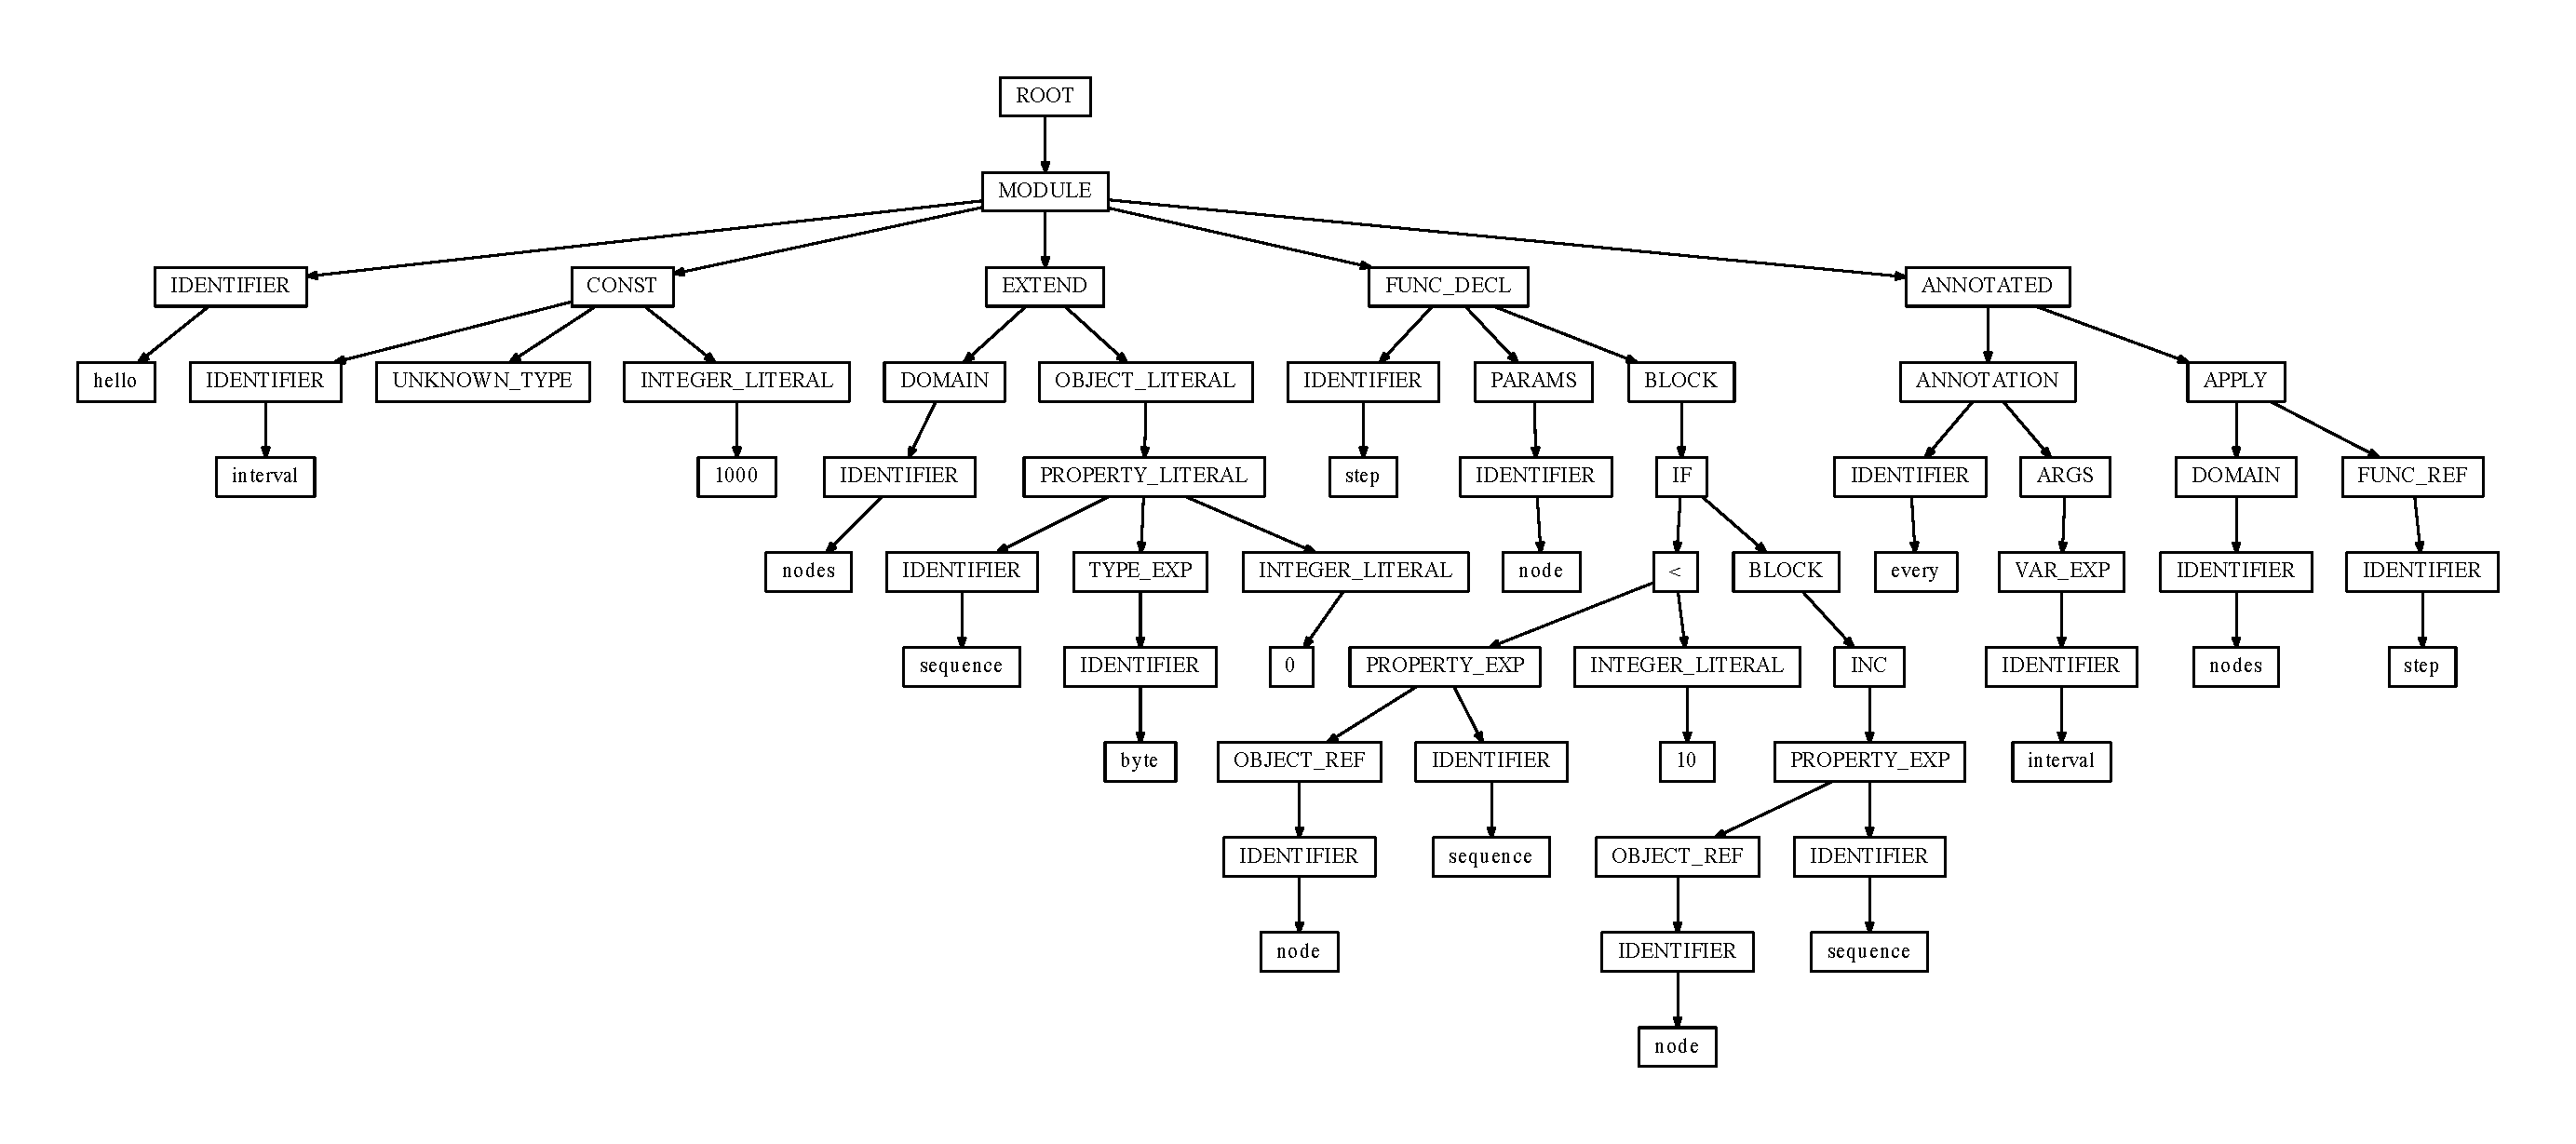
\includegraphics[width=\linewidth]{resources/hello_ast.pdf}
  \caption{De AST van het elementaire voorbeeld, \ttt{hello.foo}}
  \label{fig:devel-ast}
\end{figure}

We herkennen duidelijk de inhoud van het codevoorbeeld: op het hoogste niveau
zien we de module met een naam, de definitie van een constante, een uitbreiding
van het domein, een functie definitie en een geannoteerde applicatie van een
functie op een domein. De AST is ontdaan van alle ondersteunende syntax zoals
aanduidingen voor blokken code,\dots en bevat louter de semantische inhoud.

\subsection{Interfaces}
\label{subsection:devel-codegen-interfaces}

Voor we het SM en het CM in detail bekijken, kijken we eerst naar de interfaces
die de code generator ter beschikking stelt.

\subsubsection{foo.py}

Op het hoogste niveau biedt de generator een commandolijn interface (CLI) aan
in de vorm van een Python script: \ttt{foo.py}. Codevoorbeeld \ref{lst:foo.py-help}
toont de uitvoering van het script die een overzicht geeft van de mogelijkheden.

\begin{listing}[ht]
  \begin{minted}[linenos,frame=lines,framesep=2mm,fontsize=\footnotesize]{console}
$ source setpath.sh
$ ./foo.py --help
usage: foo.py [-h] [-v] [-c] [-i] [-g FORMAT] [-o OUTPUT] [-l LANGUAGE]
              [-p PLATFORM]
              [sources [sources ...]]

Command-line tool to interact with foo-lang and its code generation
facilities.

positional arguments:
  sources               the source files in foo-lang

optional arguments:
  -h, --help            show this help message and exit
  -v, --verbose         output info on what's happening
  -c, --check           perform model checking
  -i, --infer           perform model type inferring
  -g FORMAT, --generate FORMAT
                        output format (choices: none, ast, ast-dot, sm-dot,
                        foo, code / default: none)
  -o OUTPUT, --output OUTPUT
                        output directory (default: .)
  -l LANGUAGE, --language LANGUAGE
                        when format=code: target language (choices: c /
                        default: c)
  -p PLATFORM, --platform PLATFORM
                        when format=code: target platform (choices: moose,
                        demo / default: moose)
  \end{minted}
  \vspace{-5mm}
  \caption{Informatie over de werking van \ttt{foo.py}}
  \label{lst:foo.py-help}
\end{listing}

De CLI biedt toegang tot alle aspecten van de generator: model controle
(\ttt{check}), type deductie (\ttt{infer}), het uitvoerformaat, waar de uitvoer
moet geplaatst worden, welke taal gebruikt moet worden en voor welk platform de
generatie moet gebeuren.

De lijst van mogelijke uitvoerformaten bestaat uit: \ttt{none}, \ttt{ast},
\ttt{ast-dot}, \ttt{sm-dot}, \ttt{foo} en \ttt{code}.

Formaat \ttt{ast} toont een hierarchisch overzicht van de AST op het scherm in
tekstuele vorm, zoals weergegeven in codevoorbeeld \ref{lst:foo.py-ast}. De
uitvoer van \ttt{ast-dot} zagen we in essentie reeds eerder in figuur
\ref{fig:devel-ast}. De uitvoer is feitelijk code die als invoer kan dienen
voor GraphViz \citep{url:graphviz}, een open bron project dat zich
specialiseert in het visualiseren van graafgeori\"enteerde gegevens, zoals deze
AST met een boomstructuur. Door middel van het \ttt{dot} commando kan
vervolgens van deze code een visuele voorstelling gemaakt worden.

\begin{listing}[ht]
  \begin{minted}[linenos,frame=lines,framesep=2mm,fontsize=\footnotesize]{console}
$ source setpath.sh
$ ./foo.py -g ast examples/hello.foo 
ROOT
  MODULE
    IDENTIFIER
      hello
    CONST
      IDENTIFIER
        interval
      UNKNOWN_TYPE
      INTEGER_LITERAL
        1000
    EXTEND
...
  \end{minted}
  \vspace{-5mm}
  \caption{Tekstuele uitvoer van een AST}
  \label{lst:foo.py-ast}
\end{listing}

Overeenkomstig bestaat er ook de mogelijkheid om een visuele voorstelling te
maken van het SM, door middel van het \ttt{sm-dot} formaat. Om controles te
doen betreffende de goede verwerking van de FOO-lang broncode kan een ingelezen
set van modules ook opnieuw als FOO-code uitgevoerd worden.

Tot slot is er nog het \ttt{code} formaat, dat de generator vraagt om
effectieve code te genereren. Hierbij dienen dan ook de overige opties
eventueel ingevuld te worden: uitvoerlocatie, taal en platform.

\subsubsection{API}

Het \ttt{foo.py} Python script is slechts een CLI-verpakking rond de Python
API. Deze biedt alle functionaliteit aan in de vorm van een Python module met
een imperatieve interface. Codevoorbeeld \ref{lst:codegen-api} toont de interface
van deze module.

\begin{listing}[ht]
  \begin{minted}[linenos,frame=lines,framesep=2mm,fontsize=\footnotesize]{python}
def create_model():
  ...
  return model

def parse(string, noprint=False):
  ...
  return parser

def infer(model, silent=False):
  ...

def check(model, silent=False):
  ...

def generate(model, args):
  ...

def load(string, model=None):
  ...
  return model
  \end{minted}
  \vspace{-5mm}
  \caption{API van de code generator}
  \label{lst:codegen-api}
\end{listing}

In volgorde zien we de verschillende fasen uit het generatie proces: het
aanmaken van een (leeg) model, het parsen van de broncode, het deduceren van
onbekende types, het controleren of een model volledig in orde is en
uiteindelijk het genereren van de code. De bijkomende \ttt{load} functie
combineert de \ttt{create\_model} en \ttt{parse} functionaliteit in \'e\'en
handige functie.

De API laat toe om de generator vanuit Python aan te spreken en eventueel
verder te integreren in een uitgebreider compilatieproces, of om andere
interfaces te voorzien (visuele gebruikersinterfaces zoals bv. een
webinterface,\dots).

De API biedt toegang tot de entiteiten op het hoogste niveau, zoals de parser,
de model-entiteit uit het SM,\dots De volledige openheid van Python code laat
verder toe om dieper door te dringen en elk aspect van het bv. model te
ondervragen of zelfs te wijzigen.

Beide onderliggende modellen zijn echter volledig ondervraagbaar aan de hand
van een \emph{visitor}. Deze worden door de generator veelvuldig gebruikt,
zelfs voor kleine operaties en bieden een veel aantrekkelijkere interface om
met de modellen te werken dan het ruwweg volgen van eigenschappen en methoden
doorheen het model.

\subsection{Semantisch model}
\label{subsection:devel-semantic-model}

De AST wordt door een eerste \emph{visitor} ingeladen in het SM. Dit is in
essentie een eenvoudige vertaling van de boomstructuur naar de overeenkomstige
elementen in het SM. Het resultaat kan opnieuw gevisualiseerd worden door
middel van GraphViz, zoals weergegeven in figuur \ref{fig:hello.sm}.

\begin{figure}[ht]
  \centering
  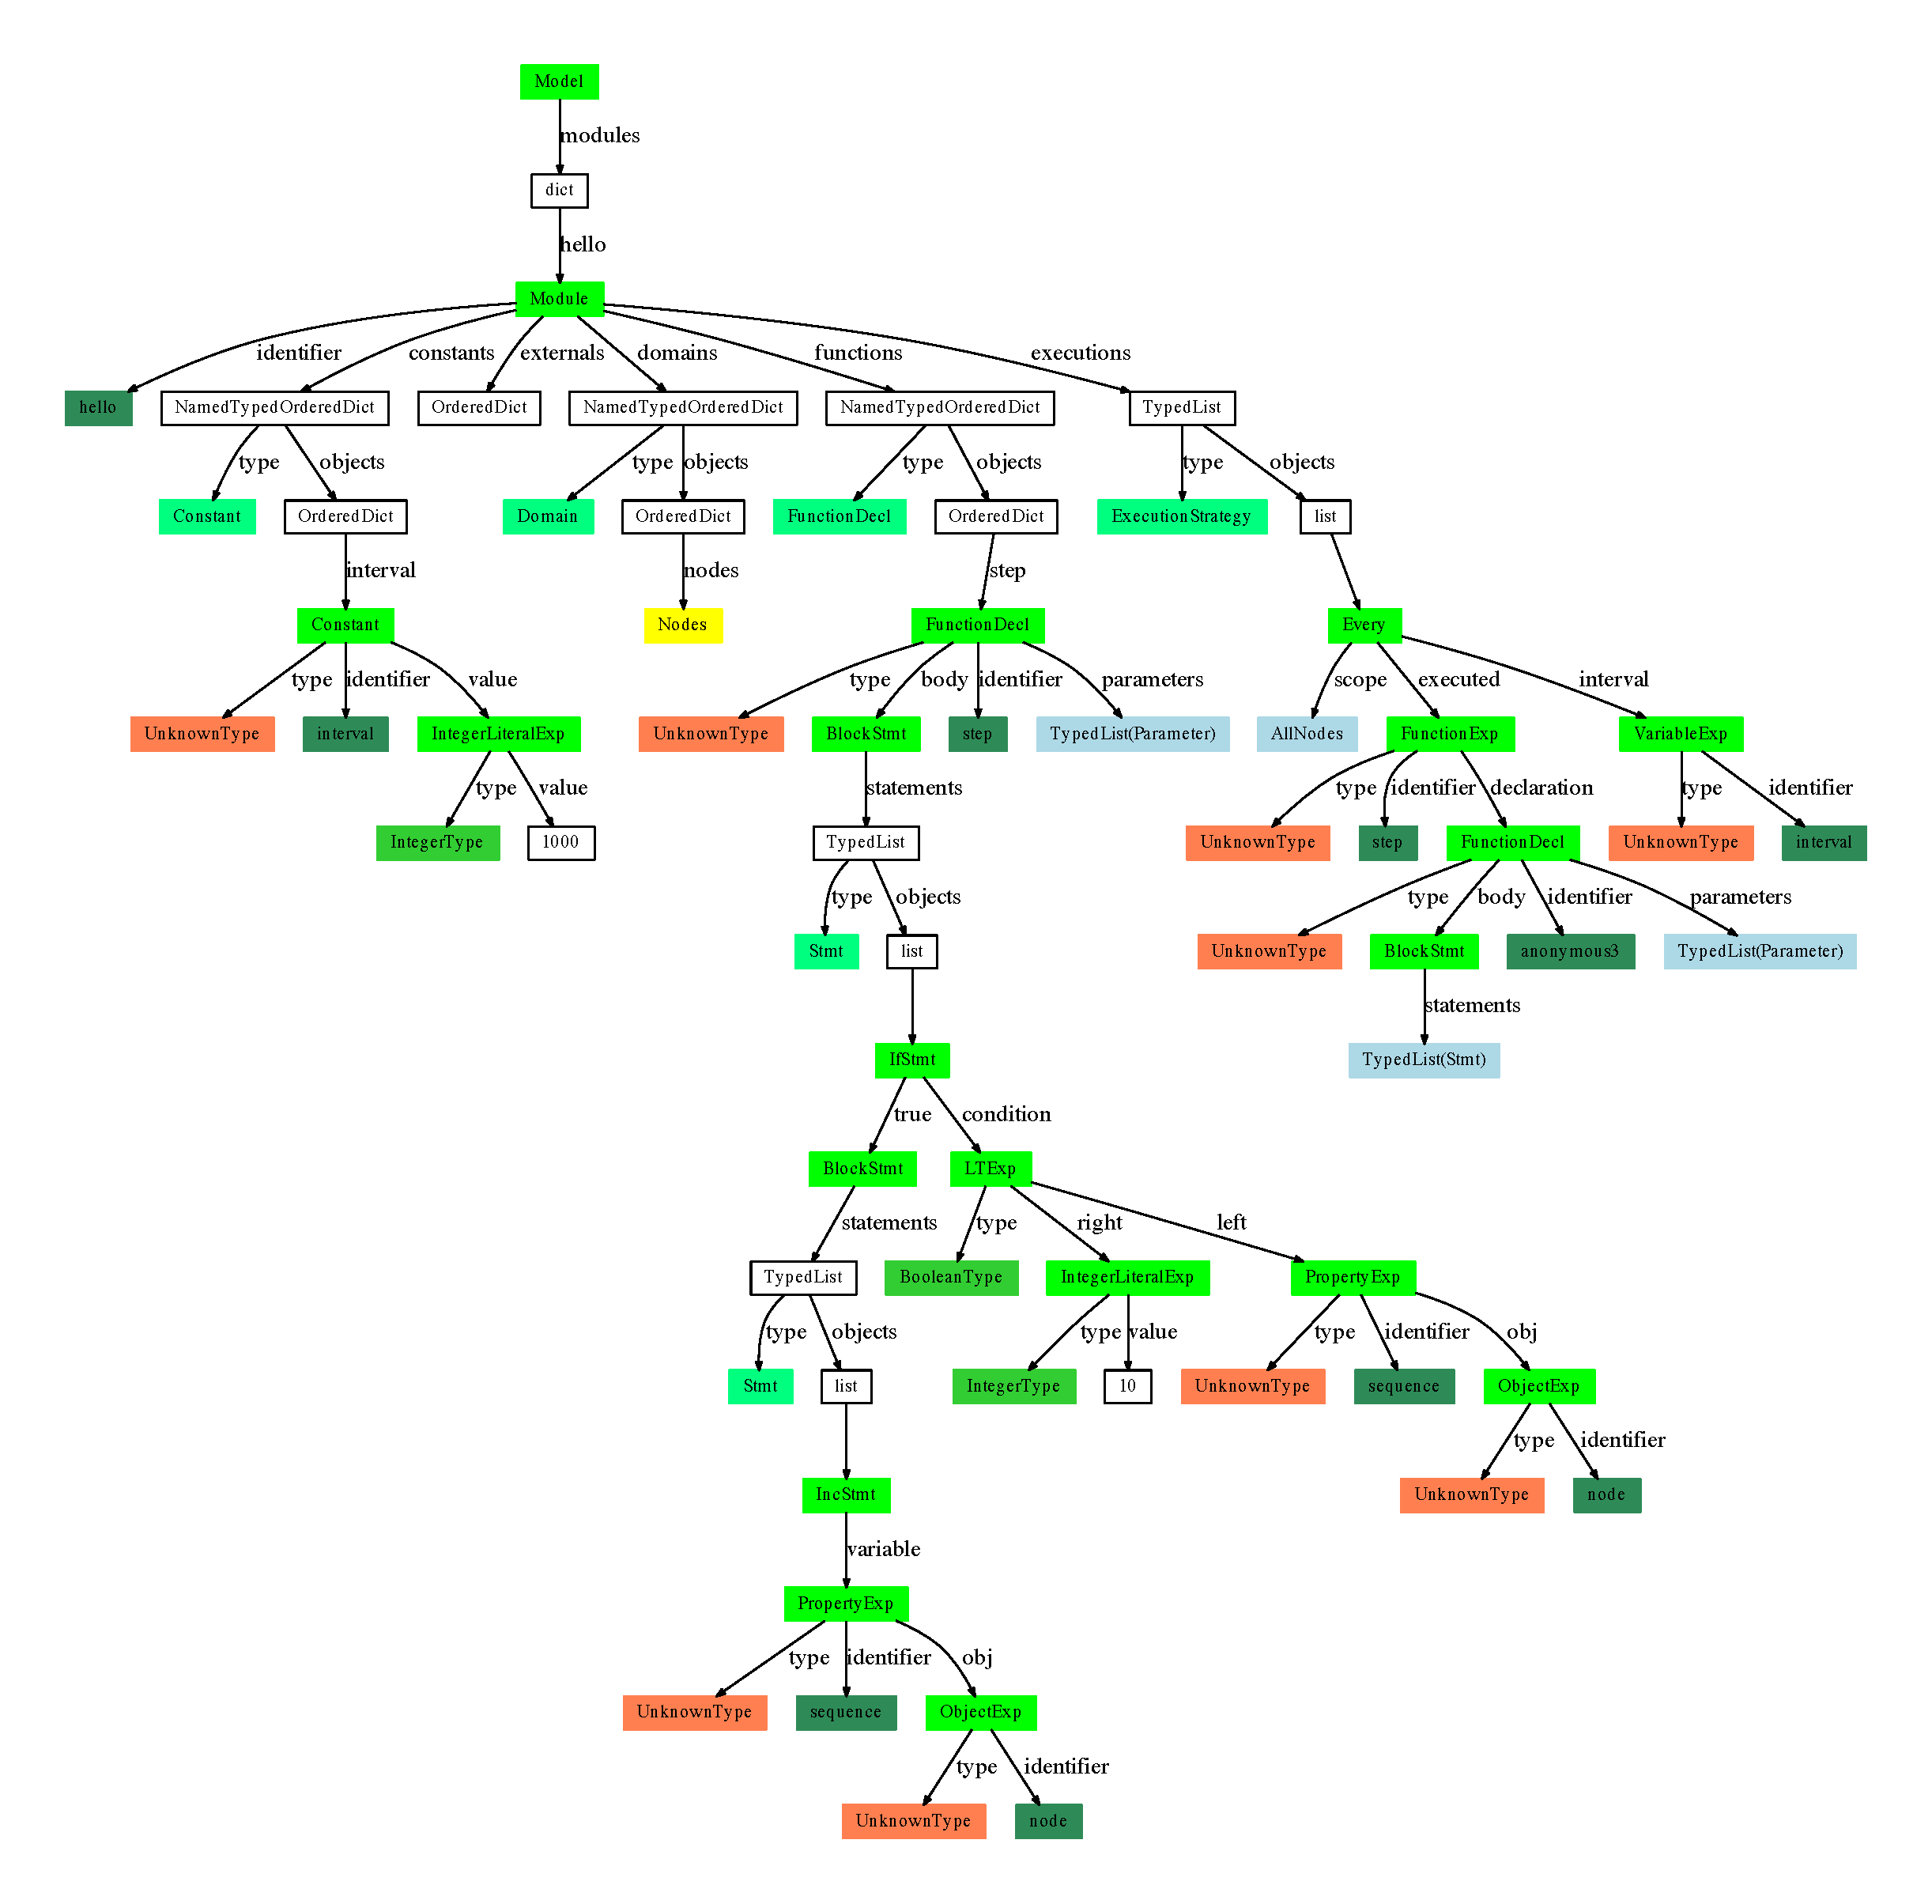
\includegraphics[width=\linewidth]{resources/hello_sm.pdf}
  \caption{Het SM van het elementaire voorbeeld, \ttt{hello.foo}}
  \label{fig:hello.sm}
\end{figure}

Bij deze visualisatie is gebruikgemaakt van een kleurencodering. Het SM kan
veel meer informatie bevatten dan de AST, zoals onder meer typering. Hierdoor
wordt de visualisatie van het SM ook een stuk groter. Dankzij de kleuren is het
makkelijker om het diagram te interpreteren.

De belangrijkste kleur is zonder meer de rode kleur. Deze geeft problemen aan
in het model. In dit geval betreft het onbekende types. Dit is in deze fase van
het generatieproces normaal aangezien typering in FOO-lang optioneel is. Deze
eerste versie van het SM bevat daarom nog niet alle types.

Een ander deel dat lijkt te ontbreken in dit diagram is de uitbreiding van het
domein. In het voorbeeld werd immers een eigenschap \ttt{sequence} toegevoegd.
Aangezien dit een uitbreiding is van het domein, zal deze terug te vinden zijn
in de eigen instantie van het domein voor deze module. In figuur
\ref{fig:hello.sm} is dit domein beperkt tot een referentie in een gele kleur.
Figuur \ref{fig:nodes.sm} toont de volledige inhoud van wat zich hierachter
verschuilt.

\begin{figure}[H]
  \centering
  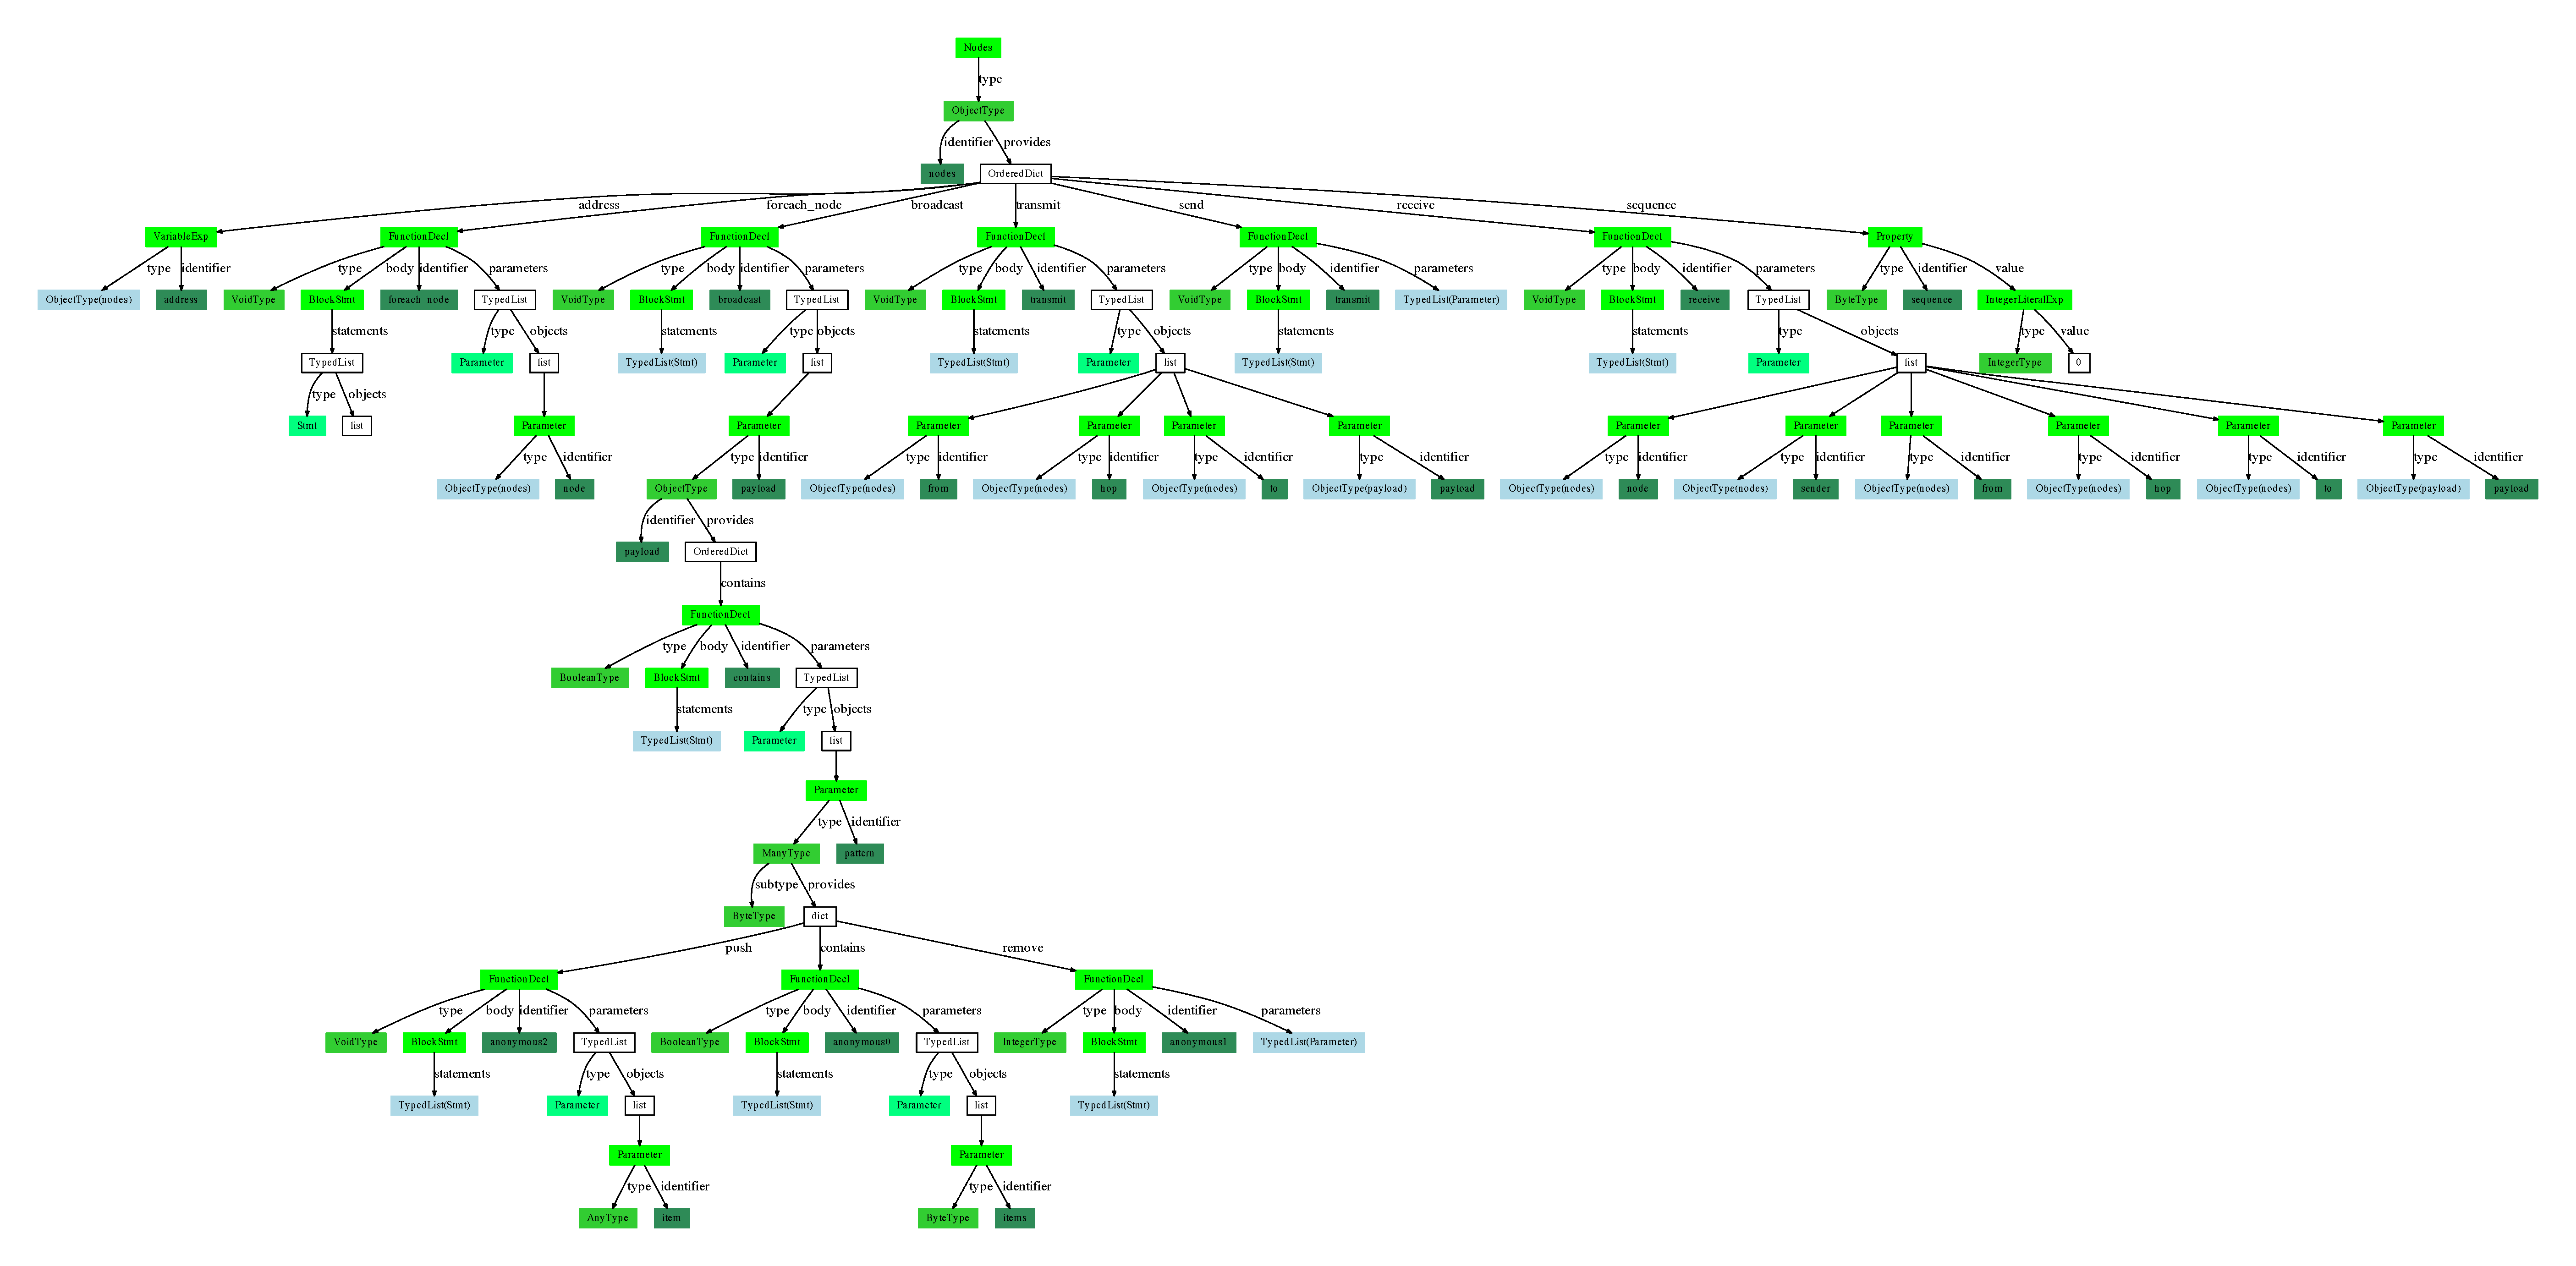
\includegraphics[angle=90,width=0.7\linewidth]{resources/nodes_sm.pdf}
  \caption{Het knopendomein in het SM voor \ttt{hello.foo} }
  \label{fig:nodes.sm}
\end{figure}

Dit is een groot stuk van het SM en behelst verschillende types en functie
declaraties die door het knopendomein ge\"introduceerd worden in het SM. Hier
zien we tevens de uitbreiding met de extra \ttt{sequence} eigenschap.

\subsubsection{Type deductie}

De volgende stap in het generatieproces bestaat erin om de nog onbekende types
te deduceren op basis van andere informatie uit het SM. Dit gebeurt aan de hand
van de \ttt{inferrer module}. Dit is een implementatie van de \emph{visitor}
voor het SM die nagaat dat alle types gekend zijn. Voor onbekende types wordt,
afhankelijk van de plaats van het type op verschillende manieren op zoek gegaan
naar een juiste typering.

De eenvoudigste methode bouwt terwijl het model doorlopen wordt een overzicht
op van gekende types die ontstaan door de declaratie van variabelen,\dots
Indien een onbekend type wordt gevonden, consulteert de \ttt{inferrer module}
dit overzicht. Indien een referentie naar een eerdere declaratie gevonden
wordt, kan het type eenvoudig gededuceerd worden.

In een aantal gevallen is de deductie niet rechtstreeks af te lezen uit
eenvoudige declaraties en moet er naar andere mogelijke combinaties gekeken
worden. Voorbeelden hiervan zijn bv. functie declaraties die gebruikt worden
als reactie op een gebeurtenis. De gebeurtenis specificeert hoe de reagerende
functie gedeclareerd is. Op basis van de omkaderende gebeurtenis moet
vervolgens het overeenkomstige prototype van de functie opgezocht en gekoppeld
worden.

Na het succesvol uitvoeren van deze type deductie zijn de voordien onbekende
types gekend en is het model volledig. Figuur \ref{fig:hello.sm-inferred} toont
hetzelfde SM als voordien, echter nu met volledig gekende typering.

\begin{figure}[ht]
  \centering
  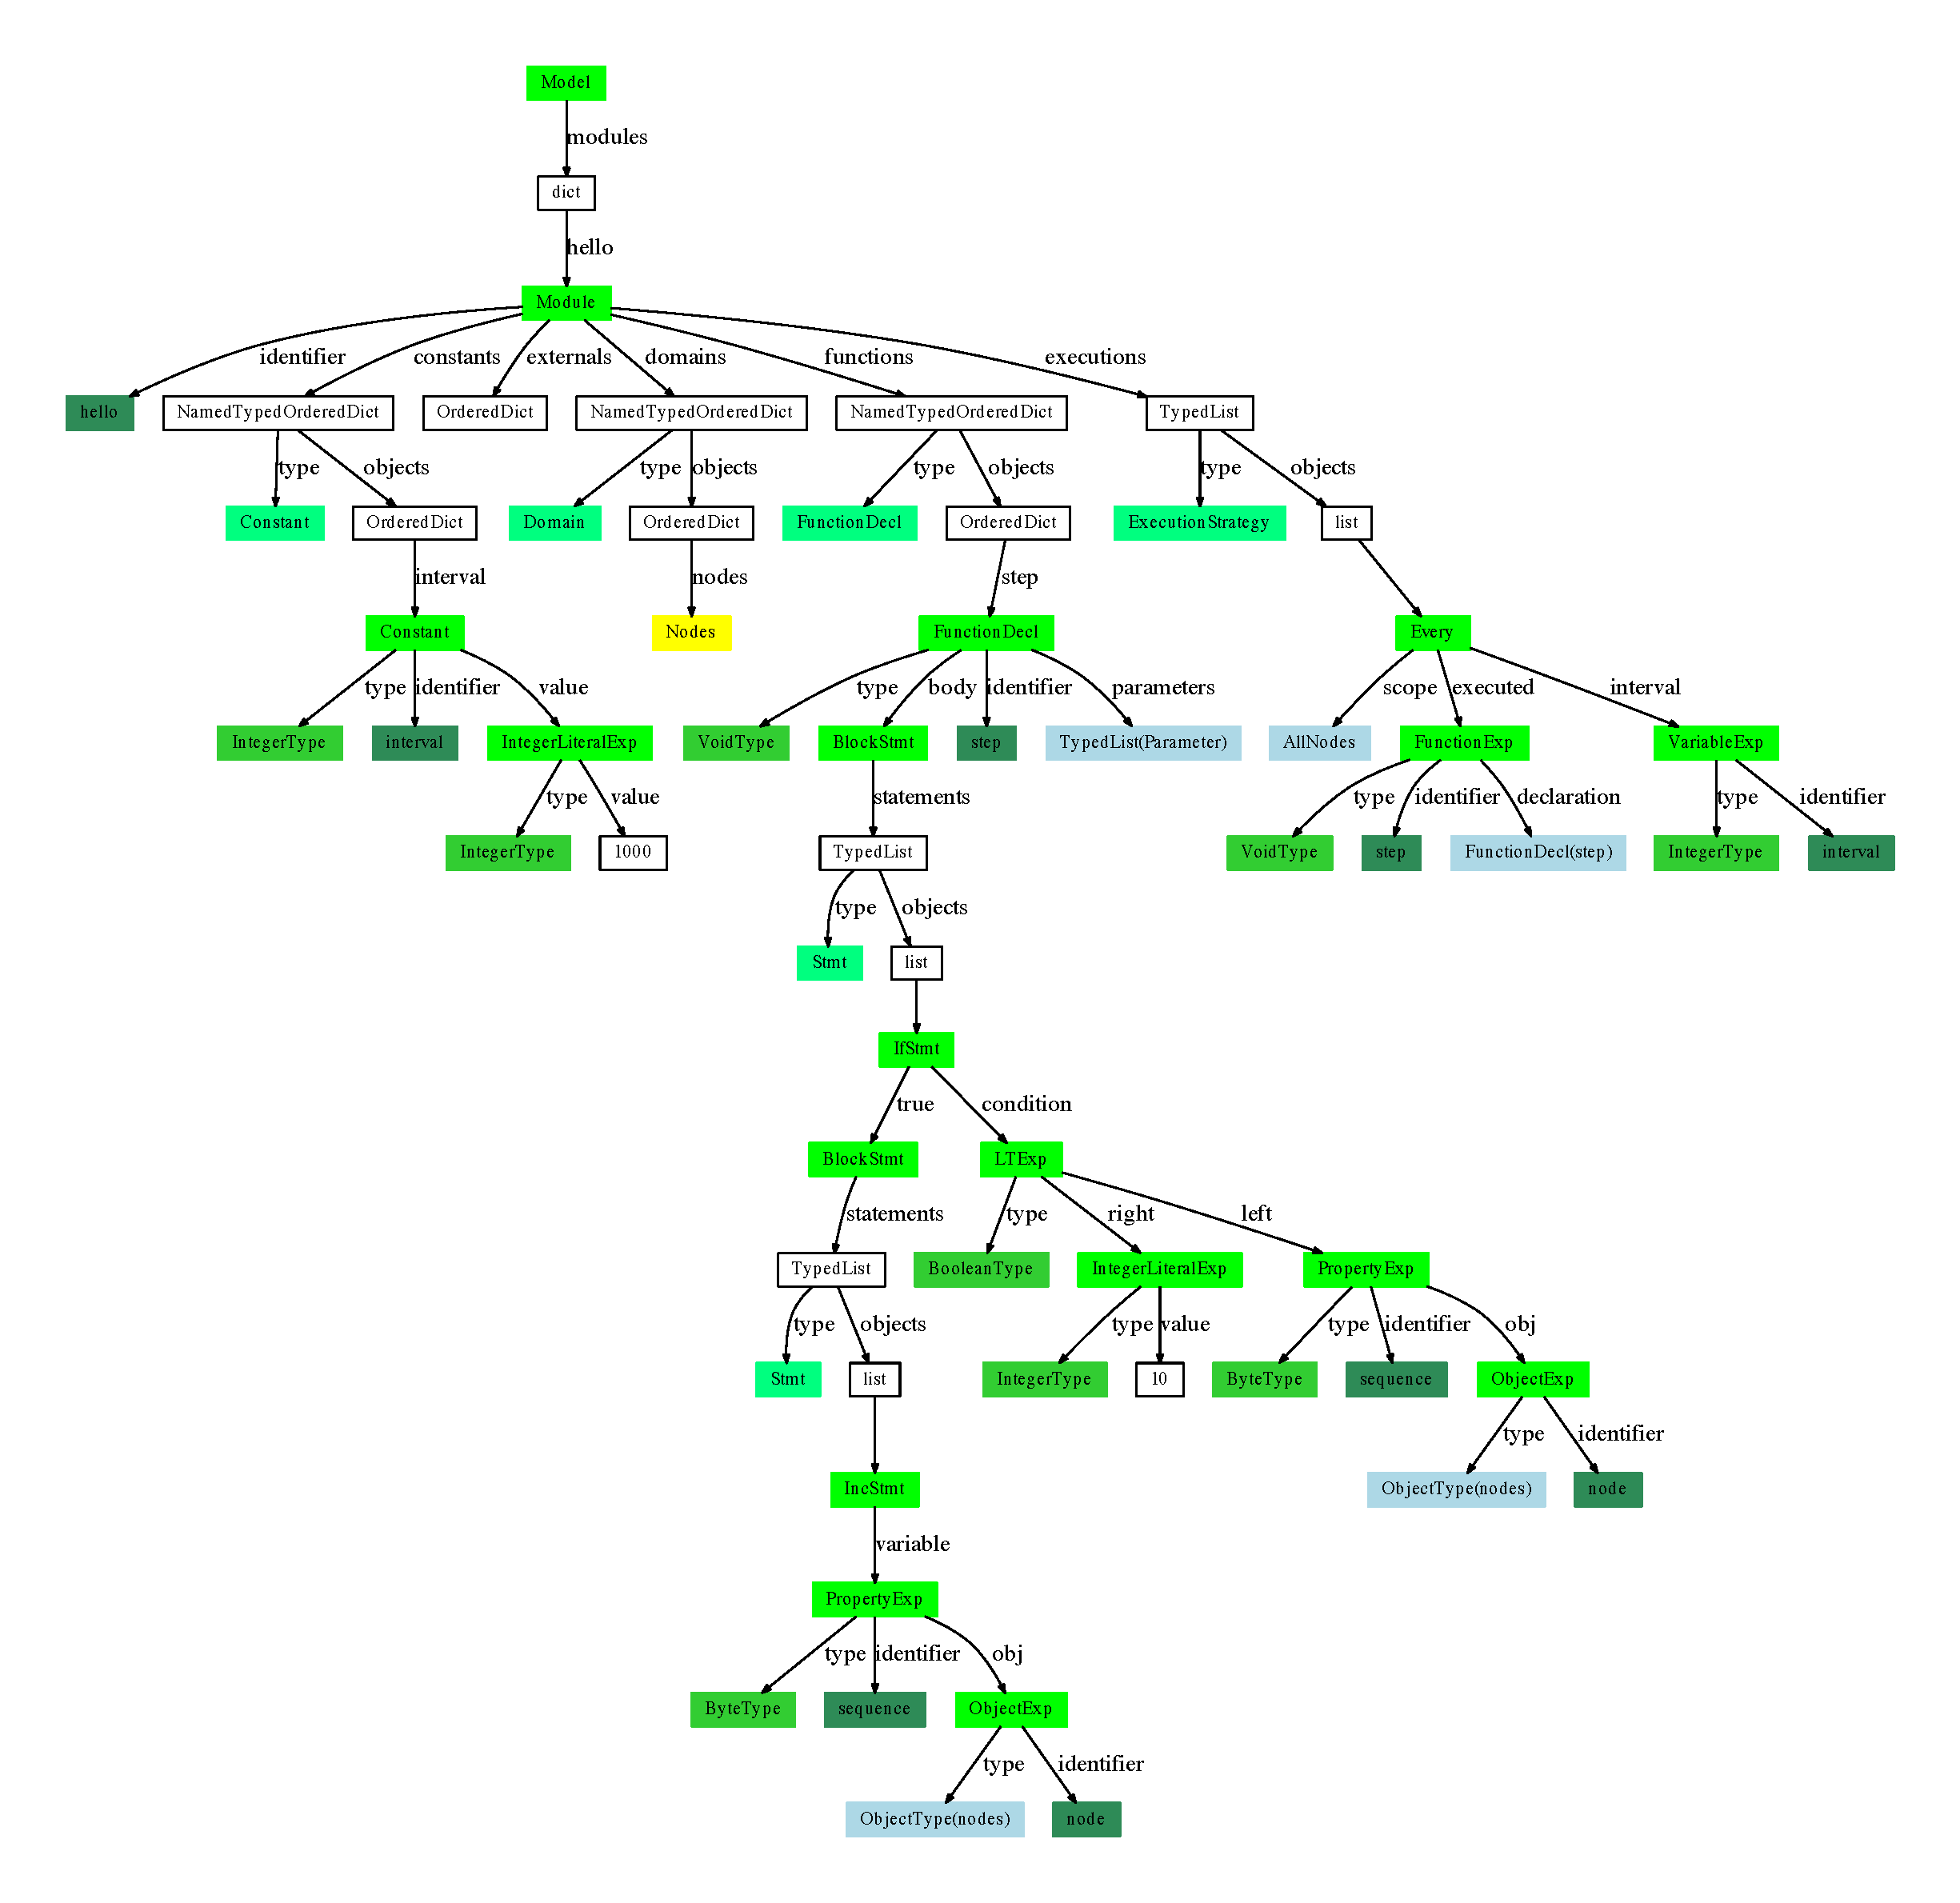
\includegraphics[width=\linewidth]{resources/hello_sm_inferred.pdf}
  \caption{Het SM van het elementaire voorbeeld, \ttt{hello.foo}, na type deductie}
  \label{fig:hello.sm-inferred}
\end{figure}

Ofschoon men verwacht dat deze fase geen structurele wijzigingen aanbrengt aan
het SM, zien we in dit geval toch dat er een vijftal elementen uit het model
verdwenen lijken te zijn. Dit is nochtans een gewoon voorbeeld van deductie. Na
het inladen van het initi\"ele model werd de (enige) uitvoeringsstrategie
gekoppeld aan een functie-expressie (\emph{FunctionExp}) genaamd, \ttt{step}.
Op dit ogenblik was er over step niets meer geweten. De declaratie van step was
wel eerder gebeurd, maar het is pas in de deductiefase dat het onbekende type
van deze functie opgezocht werd. Deel van het type is tevens de declaratie
ervan. Tijdens de deductie-fase wordt deze gekoppeld aan de eerdere declaratie,
waardoor dat in figuur \ref{fig:hello.sm-inferred} deze functiedeclaratie niet
meer volledig getoond wordt, maar nu als een referentie naar de \ttt{step}
functie opgenomen is.

\subsubsection{Model controle}

De \ttt{inferrer module} tracht alle onbekende types te deduceren. Hiermee
moeten normaal gezien de overblijvende problemen opgelost zijn. Een tweede
ondersteunende module is de \ttt{checker module} or model controle module. Deze
overloopt ook aan de hand van een \emph{visitor} het hele model en controleert
of alles in orde is.

De \ttt{checker module} is typisch nuttig bij het schrijven van FOO-lang code
en kan dienen als syntax en semantisch controle. Wanneer er bv. een schrijffout
gemaakt wordt in de naam van een variabele of functie, kan dit soms niet direct
opvallen. FOO-lang maakt bv. automatisch declaraties voor variabelen aan
wanneer zij voor het eerste gebruikt worden en nog niet eerder gedeclareerd
werden. De \ttt{checker module} kan bv. voor deze situaties waarschuwingen
geven, die kunnen helpen bij het schrijven van de FOO-lang broncode.

Ter illustratie toont codevoorbeeld \ref{lst:checker} de uitvoer van het
\ttt{hello.foo} voorbeeld. Hier is echter een \emph{fout} gemaakt in de naam
van de toegepast functie: in plaats van \ttt{step} wordt verwezen naar
\ttt{step2}.

\begin{listing}[ht]
  \begin{minted}[linenos,frame=lines,framesep=2mm,fontsize=\footnotesize]{console}
$ source setpath.sh
$ ./foo.py --check examples/hello.foo
foo-checker: failure: constant type is Unknown : interval
    stack:
      Model > Module(hello) > Constant(interval)
    env:
      interval : Constant(interval)
      
foo-checker: failure: parameter type is Unknown : node
    stack:
      Model > Module(hello) > FunctionDecl(step) > Parameter(node)
    env:
      node : Parameter(node)
        nodes : Nodes(nodes)
        interval : Constant(interval)
        step : FunctionDecl(step)
      
foo-checker: failure: function return type is Unknown : step
    stack:
      Model > Module(hello) > FunctionDecl(step)
    env:
      nodes : Nodes(nodes)
      interval : Constant(interval)
      step : FunctionDecl(step)
      
foo-checker: failure: FunctionExp type is Unknown : step2
    stack:
      Model > Module(hello) > Every(AllNodes(nodes)) > FunctionExp(step2:UnknownType)
    env:
      nodes : Nodes(nodes)
      interval : Constant(interval)
      step : FunctionDecl(step)
      
foo-checker: failure: FunctionExp has no definition. : step2
    stack:
      Model > Module(hello) > Every(AllNodes(nodes)) > FunctionExp(step2:UnknownType)
    env:
      nodes : Nodes(nodes)
      interval : Constant(interval)
      step : FunctionDecl(step)
  \end{minted}
  \vspace{-5mm}
  \caption{API van de code generator}
  \label{lst:codegen-api}
\end{listing}

\subsection{Code model}
\label{subsection:devel-code-model}

\TODO

\subsection{Transformaties}
\label{subsection:transformations}

\TODO

\subsubsection{Het visitor patroon}
\label{subsubsection:devel-visitor-pattern}

\TODO

\section{FOO-lib}
\label{section:devel-foo-lib}

\TODO

%!TEX root=masterproef.tex

\chapter{Discussie}
\label{chapter:discussie}

Inspectie van de gegenereerde code leert dat het prototype het beoogde doel
realiseert. We illustreerden dit reeds tijdens de bespreking van de
implementatie in sectie \ref{section:generation}. Hier zagen we hoe de
generator bepaalde patronen in de FOO-lang broncode omzet naar code die
tegemoetkomt aan de typische problemen die kunnen ontstaan indien
implementaties van verschillende algoritmen gewoon naast elkaar geplaatst
worden. In dit hoofdstuk gaan we echter dieper in op deze vaststelling en
trachten de kwaliteit van de oplossing te quantificeren.

Sectie \ref{section:setup} introduceert de gebruikte testopstelling en de
algoritmen die ge\"implementeerd werden voor deze evaluatie.

Sectie \ref{section:criteria} bepaalt vervolgens de evaluatecriteria en bekijkt
de theoretische resultaten die we zouden verwachten, gegeven de mogelijkheden
tot generatie die in eerdere hoofdstukken werden voorgesteld.

Sectie \ref{section:evaluation-functionals} bekijkt eerst de invulling van de
functionele criteria.

Sectie \ref{section:evaluation-non-functionals} presenteert en evalueert
vervolgens de resultaten met betrekking tot de niet-functionele criteria.

\vspace{-3mm}

\section{Opstelling}
\label{section:setup}

De evaluatie gebeurde door middel van een representatieve hardware- en
netwerkopstelling. Hierop werd een selectie van detectiealgoritmen
ge\"implementeerd. Figuur \ref{fig:setup} geeft een overzicht van de volledige
opstelling. Secties \ref{subsection:eval-hardware},
\ref{subsection:eval-software} en \ref{subsection:eval-algorithms} introduceren
respectievelijk de hardware, software en algoritmen die hier een rol spelen.

\begin{figure}[ht]
  \centering
  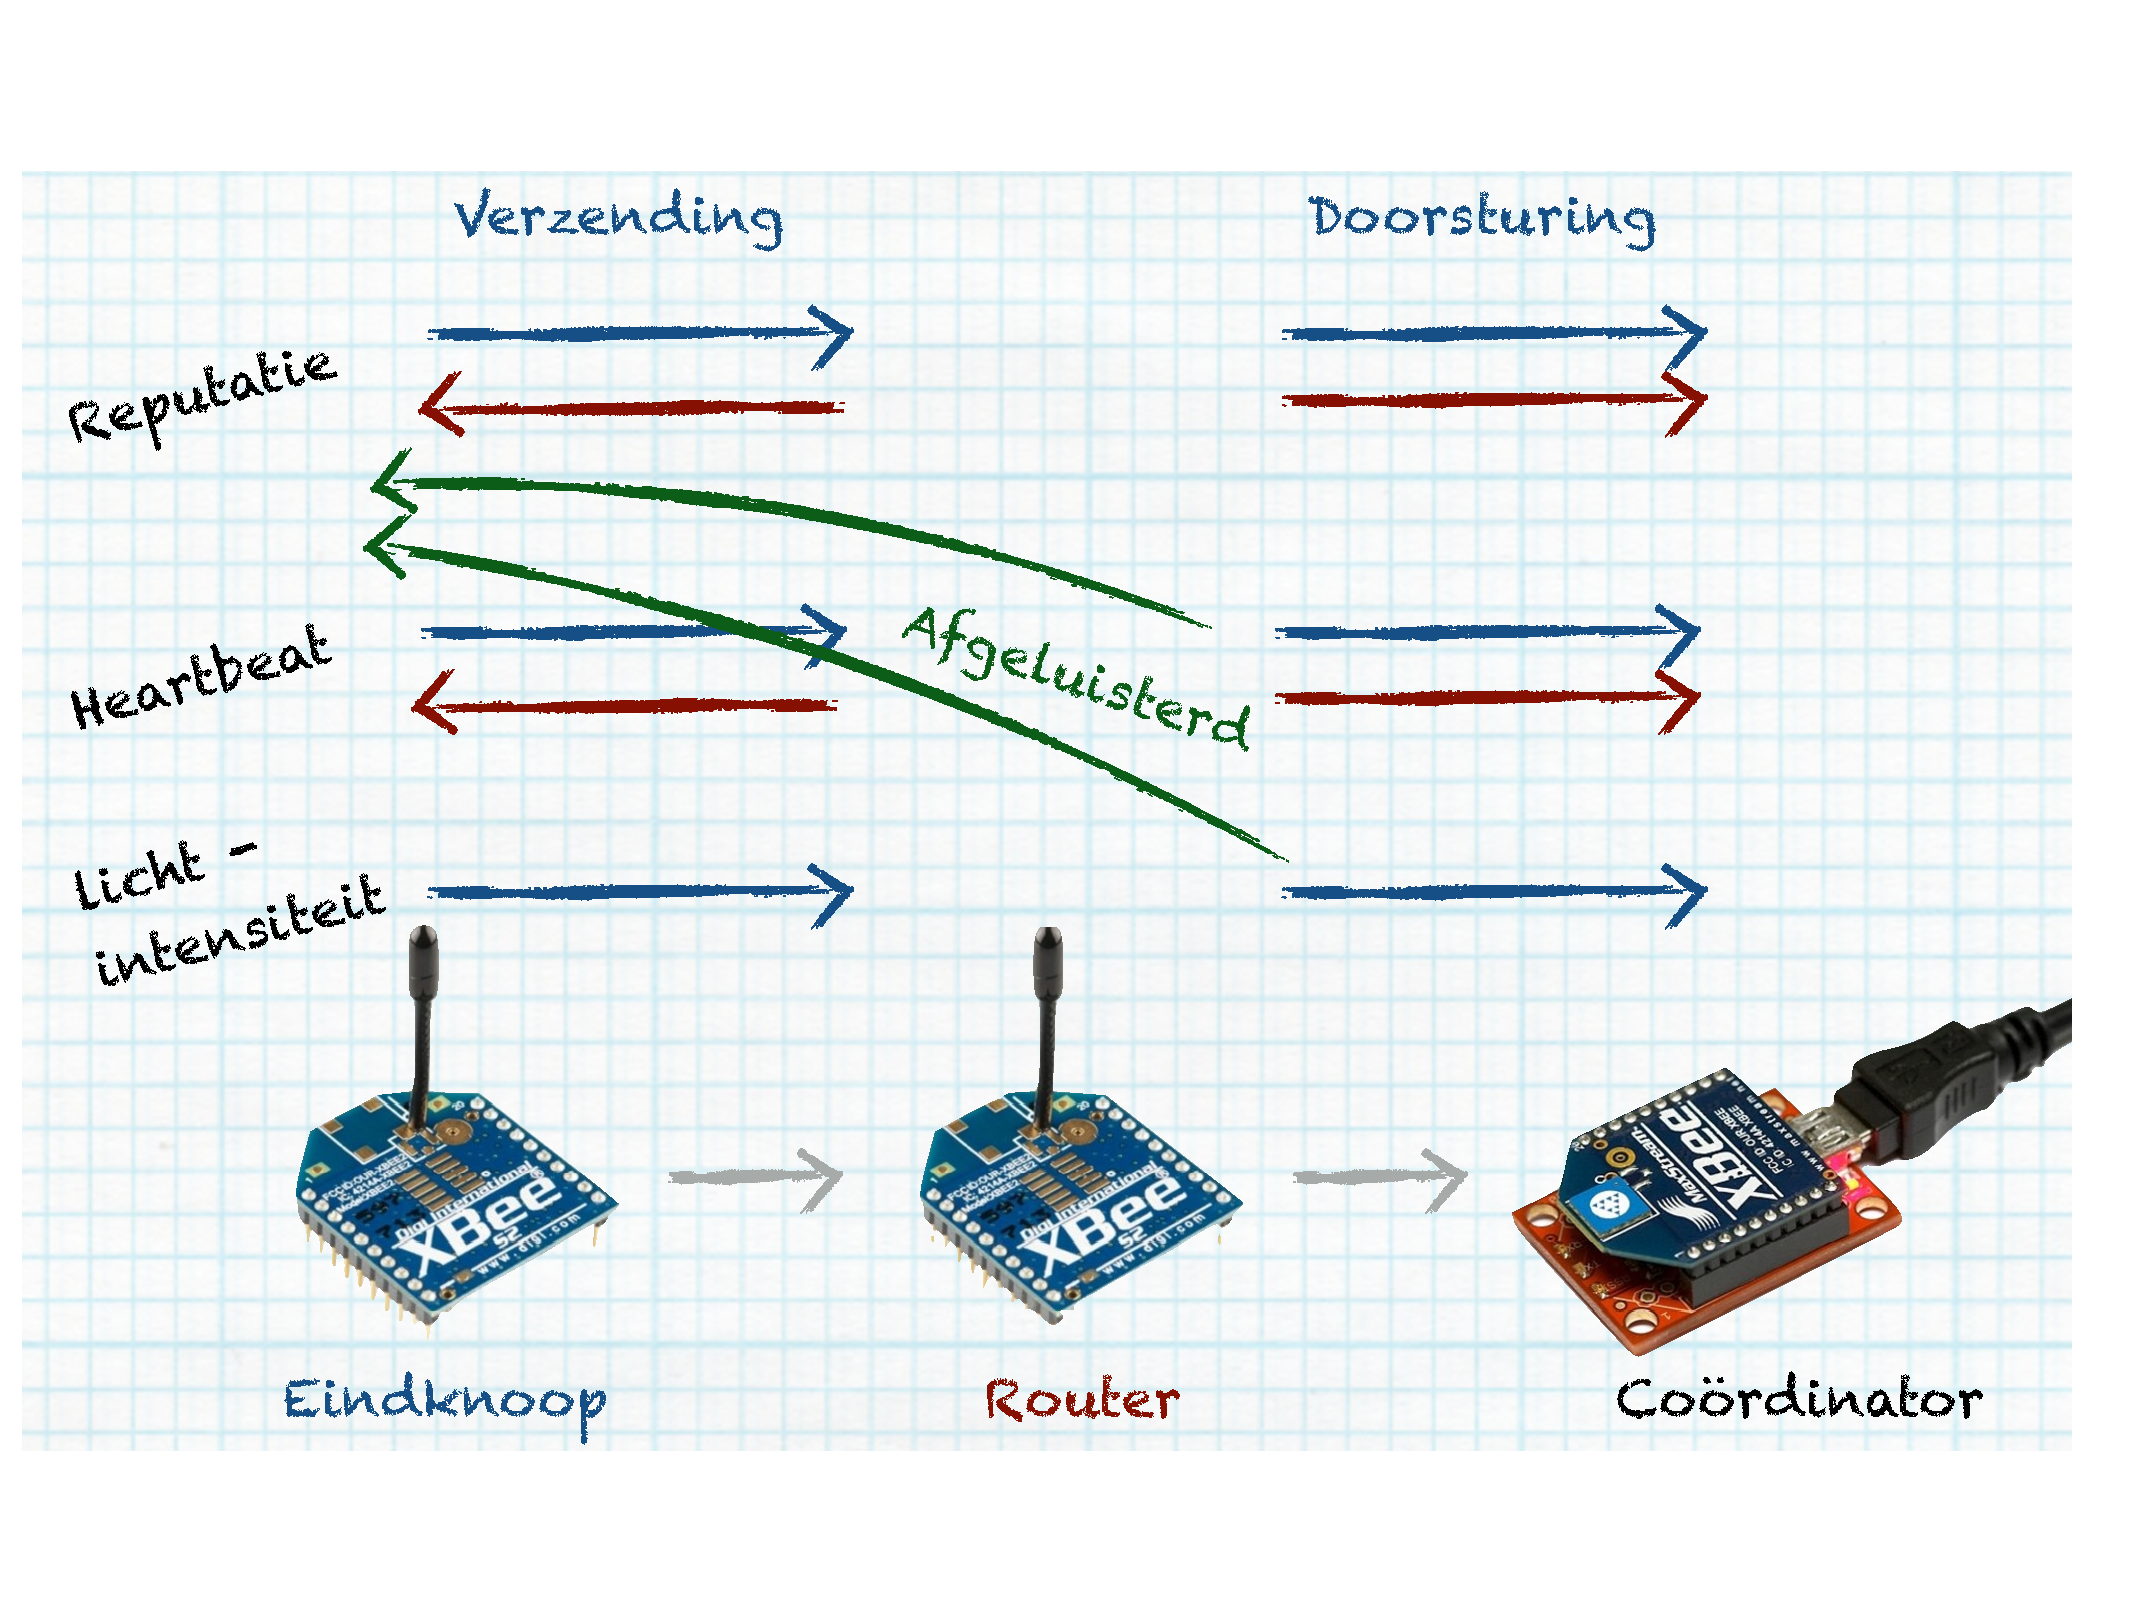
\includegraphics[width=0.75\linewidth]{resources/setup.pdf}
  \caption{Overzicht van de testopstelling met visualisatie communicatie}
  \label{fig:setup}
\end{figure}

\vspace{-5mm}

\subsection{Hardware en netwerk}
\label{subsection:eval-hardware}

Het WSN dat voor deze opstelling gerealiseerd werd, is gebaseerd op de
Zigbee-netwerkinfrastructuur en bestaat uit 3 knopen: een eindknoop, een router
en een co\"ordinator. De configuratie van de verschillende radio-modules werd
zo ingesteld dat deze topologie op kleine schaal gerealiseerd kon worded.
Hiertoe werd een extra netwerk-laag in software toegevoegd. Deze laag zorgt
o.a. voor een simulatie van het feit dat elke knoop berichten van een andere
knoop kan \emph{afluisteren}. De elementaire hardware die gebruikt werd voor
het draadloze netwerk liet dit in feite niet toe. In bijlage \ref{virtual-mesh}
wordt deze virtuele netwerklaag in meer detail toegelicht.

De sensorknopen zijn niet gebaseerd op een welbepaald bestaand platform, maar
zijn samengesteld uit een \mcu en een Zigbee-module. Er werd gebruik gemaakt
van een Atmel ATMEGA1284p \citep{datasheet:atmega1284p} en een Digi XBee 2
module \citep{manual:xbee}. Bijlage \ref{hardware-platform} bespreekt de bouw
van de sensorknoop. De keuze om geen standaard platform te gebruiken is
belangrijk. De gekozen \mcu is een veel gebruikte architectuur en komt voor in
veel hedendaagse standaard platformen en sensorknopen, zoals bv de Atmal
RZRAVEN ontwikkelkit \citep{manual:rzraven} of het Arduino open bron
electronica platform \citep{url:arduino}.

Door gebruik te maken van elementaire componenten wordt het platform herleid
tot zijn fundamentele basis. Zo kan de generator ge\"evalueerd worden in een
context die geen voordelen noch nadelen biedt. Standaard platformen komen
tevens veelal met een eigen raamwerk voor ontwikkeling of nood aan een vorm van
besturingssysteem. Vertrekken van deze elementaire basis garandeert dat elke
toevoeging van standaardisatie van het platform of toevoeging van een hoger
niveau van abstractie op softwarevlak, voordelen biedt voor de implementatie
van de generator en dit eenvoudiger maakt. Met dit platform zijn we van mening
dat er een representatieve, minimale basis bestaat waarmee de generator in
staat is om code te genereren.

\vspace{-3mm}

\subsubsection{Basis- en toepassingssoftware}
\label{subsection:eval-software}

Naast de hardware en de virtuele netwerklaag, wordt verder gebruik gemaakt van
een kleine abstractielaag boven de hardware. Met dezelfde filosofie in
gedachte, zorgt deze elementaire tussenlaag voor een situatie waarbij de eisen
die aan het onderliggende platform gesteld worden minimaal zijn. De
functionaliteit die gebruikt worden beperkte zicht tot elementaire operaties
aangaande het netwerk:

\begin{itemize}[noitemsep, topsep=0pt, partopsep=0pt]

  \item wachten tot het netwerk beschikbaar is

  \item het opvragen van het eigen netwerkadres en dat van de hoger liggende
  knoop

  \item het verzenden van een pakket
  
  \item het ontvangen van een pakket

\end{itemize}

Om de opstelling te voorzien van een functionele toepassing, werd een
lichtsensor toegevoegd aan de knopen. De toepassing van het netwerk meet op
geregelde tijdstippen de lichtintensiteit en stuurt deze naar de co\"ordinator
van het netwerk.

\subsection{Detectiealgoritmen}
\label{subsection:eval-algorithms}

Daarnaast werden twee detectiealgoritmen ge\"implementeerd: het elementaire
\emph{heartbeat} principe en een algoritme dat op basis van observaties een
waardering opbouwt omtrent de betrouwbaarheid van andere knopen. Beide
algoritmen werden in FOO-lang beschreven en zijn opgenomen in bijlage
\ref{appendix:demo-code}.

\begin{description}[noitemsep, topsep=0pt, partopsep=1pt]

  \item[Heartbeat] In het kader van het \emph{heartbeat} principe zenden
  knopen op gestelde tijdstippen een pakket uit. Andere knopen kunnen deze
  sequentie van berichten opvolgen en bij het ontbreken van deze berichten de
  beschikbaarheid van een knoop in vraag stellen. Ofschoon minimalistisch van
  aard, is het structureel toch representatief voor eenvoudige
  detectiealgoritmen die gegevens uitsturen, binnenkomende berichten verwerken
  en een beperkte status van andere knopen bijhouden en aggregeren tot een
  beslissing.

  De implementatie gebruikt ook een SHA1 hash \citep{rfc:3174} om een digitale
  handtekening toe te voegen aan het bericht. Zonder de betrouwbaarheid van
  deze aanpak in vraag te willen stellen, staat het gebruik ervan eerder in
  functie van het aantonen dat cryptografische en externe functionaliteit kan
  gebruikt worden.

  \item[Reputatie] Het tweede algoritme is een implementatie van het principe
  dat voorgesteld werd in sectie \ref{subsection:reputation}. Door op te volgen
  of een hoger liggende knoop in het netwerk, berichten effectief verder
  doorheen het netwerk stuurt, wordt statistisch bepaald of deze knoop
  betrouwbaar is of niet.

  Dit algoritme voegt nog enkele complexiteiten toe en vraagt dat arbitraire
  berekeningen kunnen uitgevoerd worden en dat de resultaten er van kunnen
  ge\"interpreteerd worden. Ook wordt hier de complexiteit toegevoegd waarbij
  omgegaan moet worden met volledige netwerkpakketten.

\end{description}

\vspace{-3mm}

\subsubsection{Configuratie}

De configuratie van beide algoritmen is natuurlijk van belang. Een configuratie
die niet resulteert in een concurrentie tussen beide algoritmen zal weinig tot
geen optimalisatie laten optekenen.

De mogelijkheden tot configuratie liggen in de tijden tussen twee uitvoeringen
van een functioneel aspect van het algoritme. In beide gevallen gaat dit om een
tussentijd vooraleer het algoritme zelf een bericht uitstuurt en de tussentijd
waarop een evaluatie van de geaggregeerde informatie gebeurt. Het eerste aspect
bepaalt de synchroniciteit van het uitsturen van berichten en of er
mogelijkheid is tot samennemen van berichten om zo het draadloze netwerk te
ontlasten. Het punt van evaluatie bepaalt of het overlopen van alle gekende
knopen voor beide algoritmen tegelijk kan gebeuren of niet.

Om een situatie af te dwingen waar de voordelen van de oplossing zich kunnen
manifesteren, werd geopteerd voor volgende configuratie:

\begin{itemize}[noitemsep, topsep=0pt, partopsep=0pt]

  \item de tijd tussen twee opeenvolgende \emph{heartbeats}: 3s

  \item de tijd tussen twee opeenvolgende verzendingen i.v.m. reputatie: 7,5s

  \item in beide gevallen: de tijd tussen twee opeenvolgende evaluaties: 5s

\end{itemize}

\vspace{-3mm}

\section{Evaluatiecriteria}
\label{section:criteria}

De doelstelling om de impact van de introductie van een IDS in een WSN te
verlagen is de basis voor de evaluatiecriteria. Bij het uitdiepen van de
probleemstelling in hoofdstuk \ref{chapter:probleemstelling} werd het
ontwikkelingsproces gevolg van de hardware en het onderzoek tot de software en
de uitbating. Hieruit leiden we de volgende functionele en niet-functionele
criteria.

\vspace{-3mm}

\subsection{Functionele criteria}

Elk van de ontwikkelde componenten in deze masterproef dient een functioneel
doel:

\begin{description}[noitemsep, topsep=0pt, partopsep=1pt]

  \item[Expressiviteit] Vanuit functioneel oogpunt moet de voorgestelde taal in
  staat zijn om de beschrijving van een representatieve selectie van
  detectiealgoritmen mogelijk te maken. Concreet moet het mogelijk zijn om met
  FOO-lang de voorgestelde algoritmen correct en zonder essenti\"ele omwegen
  te implementeren.

  \item[Automatiseerbaarheid] De codegenerator moet het mogelijk maken om op
  een volledig geautomatiseerde manier een IDS toe te voegen aan een te
  integreren toepassing.

\end{description}

\vspace{-3mm}

\subsection{Niet-functionele criteria}

De niet-functionele criteria hebben betrekking op de impact van het IDS op de
middelen van de sensorknopen. In essentie komt dit neer op het energieverbruik.
We vertalen dit concept in deze context naar twee overeenkomstige en direct
be\"invloedende factoren: het gebruik van de draadloze radio en de tijd om
\'e\'en cyclus van de \emph{event loop} te doorlopen. Het gebruik van de radio
wordt verder opgesplitst in het aantal verzonden pakketten en de hoeveelheid
aan gegevens die worden verstuurd.

\begin{description}[noitemsep, topsep=0pt, partopsep=0pt]
  
  \item[Aantal verzonden netwerkpakketten] Het aantal verzonden pakketten
  bepaalt hoe frequent de radio effectief moet zenden. Dit is typisch het
  duurste wat betreft energieverbruik. Het verminderen van het aantal pakketten
  heeft dus een rechtstreekse relatie met het energieverbruik.

  \item[Aantal verzonden bytes] Het opvolgen van het aantal bytes die effectief
  verstuurd worden is van belang om in te schatten of de eventuele winst door
  een afname van het aantal verzonden pakketten niet gecompenseerd wordt door
  een toename in het aantal effectief verzonden bytes.

  \item[Lengte event loop] De doorlooptijd van \'e\'en cyclus van de
  \emph{event loop} bepaalt hoe lang de \mcu effectief actief is. Typisch wordt
  op het einde van elke cyclus een periode ingelast van niet-activiteit. De
  cyclus plus de rustperiode zijn een constante, waardoor het aandeel van de
  cyclus een relatieve impact heeft op het energieverbruik.
  
\end{description}

Naast deze drie energie-gebonden criteria kunnen we nog een vierde criterium in
beschouwing nemen, nl. de grootte van de resulterende code die naast de
applicatiecode moet ge\"installeerd worden op de sensorknoop.

Dit is een noodzakelijk kwaad, want het is evident dat de introductie van een
IDS een impact zal hebben op dit vlak. We moeten dus opnieuw een vergelijking
maken met de manuele situatie en kijken hoeveel de gegenereerde code eventueel
groter is.

\vspace{-3mm}

\subsection{Theoretische evaluatie}

Gegeven de doelstellingen en de configuratie is het mogelijk een voorspelling
te maken van bepaalde van de niet-functionele criteria. Wanneer we een periode
van 90 seconden in beschouwing nemen en de activiteiten van de algoritmen
hierbinnen uitzetten kunnen we het aantal verzonden netwerkpakketten berekenen.

De toepassing verstuurt om de 5 seconden een meting van de lichtsensor. Dit
resulteert in 18 netwerkpakketten. Het \emph{heartbeat} algoritme verstuurt
elke 3 seconden een pakket. Dit resulteert in 30 pakketten. Het
reputatie-gebaseerde algoritme verstuurt informatie om de 7,5 seconde, dus nog
eens 12 pakketten.

Over een periode van 90 seconden verwachten we dus dat er 18 + 30 + 12 = 60
pakketten verzonden worden.

Indien we aannemen dat de generator er effectief voor zorgt dat berichten die
dicht bij elkaar verzonden worden, gebundeld worden in \'e\'en pakket, dan zal
zich deze situatie aanbieden op gemeenschappelijk veelvouden van 3 en 7,5.
Concreet zal dit zijn op de veelvouden van 15, ofwel op 6 ogenblikken binnen de
periode van 90 seconden. We zouden bij de gegenereerde code dus een reductie
van 6 pakketten moeten kunnen optekenen.

\vspace{-3mm}

\section{Evaluatie van de functionele criteria}
\label{section:evaluation-functionals}

De twee functionele criteria focussen elk op \'e\'en van de twee grote
componenten die binnen de scope van deze masterproef vallen: FOO-lang en de
codegenerator.

\vspace{-3mm}

\subsection{Een derde algoritme}

Om FOO-lang zelf te evalueren werd een derde algoritme beschreven. Hierbij werd
nagegaan welke uitbreidingen of aanpassingen aan FOO-lang nodig waren om dit
derde algoritme op een gelijkwaardige manier te kunnen beschrijven.

Het algoritme in kwestie is het co\"operatieve algoritme beschreven in bijlage
\ref{section:cooperation-algorithm}. De experimentele beschrijving is terug te
vinden in bijlage \ref{lst:cooperation.foo}.

De conclusie van deze oefening is, dat er nog enkele typische constructies
ontbreken aan FOO-lang, wat in de lijn van de verwachting ligt. De meeste
tekorten zijn echter te wijten aan de minimale implementatie van de voorziene
mogelijkheden.

De concepten van de taal blijven overeind en de aanpassingen zijn meestal
uitbreidingen van bestaande constructies met bijkomende mogelijkheden of een
andere scope.

\vspace{-3mm}

\subsection{De generator}

De generator biedt met een API en een CLI toepassing een uitermate flexibele
interface naar de buitenwereld toe. Op deze manier is integratie in een
ontwikkelingsproces zeer vlot realiseerbaar. Bij wijze van illustratie is elke
test die uitgevoerd werd voor deze masterproef op te starten met \'e\'en enkele
oproep van een door een \emph{Makefile} georganiseerd generatie-, compilatie-
en installatieproces.

Een ander aspect dat van belang is in de context van de generator is de
uitbreidbaarheid. Bij het prototype is uitgegaan van een minimalistische
situatie met een \emph{event loop}. Indien men bv. ondersteuning zou willen
inbouwen voor Contiki of een ander besturingssysteem dient hiervoor een nieuwe
Python module geschreven te worden die mee de vertaling dient te doen aan de
hand van model transformaties.

Dit vraagt extra werk en een juiste inschatting van de hoeveelheid is zeer
platformafhankelijk. Hier kan slechts een indicatie gegeven worden op basis van
de ervaring bij het ontwikkelen van de software voor de evaluatie. Het
schrijven van een manuele versie op basis van enkele losse modules geeft een
goed beeld van hoe de integratie dient te gebeuren. Mits een korte analyse van
deze manuele code en een koppeling naar de typische concepten die FOO-lib
aanbiedt, kan de creatie van zo'n module vlot gebeuren. Dit is tevens een
\'e\'enmalige investering die zichzelf snel terugbetaalt bij elke volgende
generatie.

\vspace{-3mm}

\section{Evaluatie van niet-functionele criteria}
\label{section:evaluation-non-functionals}

Voor deze evaluatie werd zowel een volledig manuele implementatie gemaakt als
een gegenereerde. Beide werden opgebouwd met een zelfde programmeerstijl en
maakten geen gebruik van enige voorkennis omtrent de algoritmen. De manuele
implementatie bestaat uit een basisapplicatie en twee modules voor de
algoritmen.

Deze modules werden vervolgens sequentieel ingevoegd in de basisapplicatie,
zoals dit het geval zou zijn indien men bestaande implementaties kon
hergebruiken. Dit resulteert structureel in twee oproepen naar de modules
vanuit de \emph{event loop} en twee oproepen wanneer een bericht ontvangen
wordt.

\vspace{-3mm}

\subsection{Metingen}

Het tellen van het aantal verzonden pakketten en bytes werd toegevoegd aan de
minimale abstractielaag en is dus een constante bijkomende belasting in alle
gevallen.

Om de doorlooptijd van de event loop te meten, werd het aantal cycli dat de
\emph{event loop} doorliep gemeten gedurende een interval van 15 seconden.
Hieruit werd de doorlooptijd van \'e\'en cyclus berekend. De reden van deze
opstelling is het feit dat de \mcu slechts een kloksnelheid heeft van 8MHz.
Hiermee is het mogelijk om aan de hand van \emph{interrupts} een virtuele klok
te bouwen die milliseconden kan meten. Een grotere precisie, bv. microseconden,
zal een te groot deel van de rekentijd van de \mcu vragen, waardoor de
toepassing niet genoeg tijd meer krijgt om effectief te werken.

Naast deze aanpak werd ook gebruikgemaakt van een \emph{logic analyser}. Door
aan het begin van een oproep naar een module van een detectiealgoritme een
spanning aan te leggen op \'e\'en van de uitvoerpinnen van de \mcu en deze op
het einde van de oproep opnieuw weg te nemen, kunnen we deze verschillen van
buitenaf meten. Dit laat toe om zelfs verschillen op een
sub-microseconde-schaal te meten.

Met de beschikbare middelen was het niet mogelijk om een totaalbeeld te vormen
over een periode van 90 seconden, maar de meting liet wel toe om de situatie
waarbij in een cyclus van de event loop geen enkele actie ondernomen werd door
het IDS, in kaart te brengen. Deze situatie toont de minimale, constante extra
belasting die het IDS met zich meebrengt.

\vspace{-3mm}

\subsection{Resultaten}

Tabellen \ref{tbl:manual} en \ref{tbl:generated} tonen de ruwe metingen voor
respectievelijk de manuele en de gegenereerde implementatie. De verschillende
niet-functionele criteria worden voor de verschillende configuraties uitgezet.
De eerste situatie is die van de naakte applicatie, zonder enige vorm van IDS.
Dit is de referentie voor de andere configuraties. Daarnaast zijn drie
configuraties geplaatst: \'e\'en met alleen het \emph{heartbeat} algoritme
toegevoegd, \'e\'en met het reputatie-algoritme toegevoegd en \'e\'en met beide
algoritmen.

Naast de ruwe meetwaarde is tevens een procentuele vergelijking met de
referentie opgenomen om de impact beter te quantificeren.

\begin{table}[H]
  \centering
  \begin{tabular}{l|r|rr|rr|rr}
  \hline
      & zonder & \multicolumn{2}{c|}{heartbeat} & \multicolumn{2}{c|}{reputatie} & \multicolumn{2}{c}{beide} \\
  \hline
  \hline

aantal pakketten      &    20    &    51    & 255\% &    32    & 160\% &    63    & 315\% \\
aantal bytes          &   476    &  1933    & 406\% &   860    & 181\% &  2317    & 487\% \\
bytes/pakket          &    23.80 &    37.90 & 159\% &    26.88 & 113\% &    36.78 & 155\% \\
doorlooptijd ($\mu$s) &    48    &    94    & 196\% &    88    & 183\% &   149    & 310\% \\
grootte (bytes)       & 10500    & 15530    & 148\% & 13306    & 127\% & 18334    & 175\% \\

  \hline
  \end{tabular}
  \caption{Resultaten voor de manuele implementatie}
  \label{tbl:manual}
\end{table}

Wanneer we de referentie bij de manuele implementatie bekijken zien we dat er
inderdaad zoals verwacht (ongeveer) 19 pakketten verstuurd zijn.\footnote{Het
bijkomende pakket is toe te schrijven aan een bijkomend pakket dat tijdens het
initialiseren van het virtuele netwerk gebruikt wordt door de eindknoop om de
hoger liggende knoop te vinden.} Het gemiddeld aantal bytes per frame is
(ongeveer) 24. Een lichtmeting bestaat uit 2 bytes. Daarnaast worden er 6 extra
bytes gebruikt door de implementatie van het virtuele netwerk. Het Zigbee
pakketformaat voegt nog eens 16 bytes toe \citep{alliance2012zigbee}. De totale
som, 2 + 6 + 16 is inderdaad 24\footnote{De ogenschijnlijke fout op de waarde
is opnieuw toe te schrijven aan het initi\"ele extra pakket. Dit is slechts 4
bytes groot, heeft geen bijkomende adresinformatie van het virtuele netwerk en
heeft verder alleen nog 16 bijkomende bytes van het Zigbee-protocol. Zo komt
het op 20 bytes. Opgeteld bij 19 $\times$ 24 = 456 geeft dat inderdaad 476.}.

Door de introductie van het IDS stijgen deze waarden natuurlijk. We berekenden
reeds dat de introductie van een \emph{heartbeat} een bijkomende 30 pakketten
betekent en dat voor de communicatie voor het uitwisselen van
reputatie-informatie er 12 extra pakketten nodig zijn. We zien deze getallen
nagenoeg exact terugkomen in de meeteresultaten: in het geval van het
\emph{heartbeat} algoritme is er \'e\'en pakket meer verzonden. Dit was te
wijten aan een tweede initialisatie-pakket voor het opzetten van het virtuele
netwerk.

We merken verder op dat de combinatie van de twee algoritmen letterlijk een
sommatie is van de individuele impact. Dit is logisch en het bevestigt de
veronderstelling. In het geval van de doorlooptijd ligt deze zelfs nog iets
hoger. In plaats van 48 + 46 + 40 = 134 $\mu$s is de doorlooptijd zelfs 149
$\mu$s.

Tot slot zien we dat de manuele introductie van het IDS een vergroting van de
te installeren code van 75\% betekent. In absolute cijfers een kleine 8
kilobyte (KB).

\vspace{-3mm}

\subsubsection{Gegenereerde code}

Tabel \ref{tbl:generated} toont exact dezelfde gegevens, maar dan voor de
gegenereerde code.

\begin{table}[H]
  \centering
  \begin{tabular}{l|r|rr|rr|rr}
  \hline
      & zonder & \multicolumn{2}{c|}{heartbeat} & \multicolumn{2}{c|}{reputatie} & \multicolumn{2}{c}{beide} \\
  \hline
  \hline
  
aantal pakketten      &    20	   &    49	  & 245\%	&    32	   & 160\% &    55	  & 275\% \\
aantal bytes          &   476	   &  1897	  & 399\%	&   884	   & 186\% &  2161	  & 454\% \\
bytes/pakket          &    23.80 &  	38.71	& 163\%	&    27.63 & 116\% &    39.29	& 165\% \\
doorlooptijd ($\mu$s) &    48    &   121	  & 252\%	&   121	   & 252\% &   138	  & 288\% \\
grootte (bytes)       &	10496	   & 18352	  & 175\%	& 16376	   & 156\% & 20998	  & 200\% \\

  \hline
  \end{tabular}
  \caption{Resultaten voor de gegenereerde implementatie}
  \label{tbl:generated}
\end{table}

Hier merken we op dat de gegenereerde referentie-implementatie nagenoeg perfect
overeenkomt met de manuele referentie-implementatie\footnote{De vier bytes
verschil zijn vermoedelijk te wijten aan twee bijkomende ongebruikte
functiedeclaraties in de manuele code. Dit werd omwille van het marginale
verschil niet verder onderzocht.}.

Dezelfde getallen als bij de manuele implementatie zien we terugkomen voor het
aantal verzonden pakketten\footnote{Bij het \emph{heartbeat} algoritme werd er
geen extra pakket bij intialisering verstuurd en werd 1 pakket net niet meer
meegeteld op het einde van de 90 seconden.}.

Een eerste verschil merken we echter op bij het aantal pakketten in het geval
dat beide algoritmen actief zijn. In theorie verwachtten we hier 6 pakketten
minder. Het verschil is 8. Dit is te wijten aan een extra initialiseringspakket
bij de manuele versie en een opnieuw een pakket dat net niet meegeteld werd.

Met een lengte van 20 bytes, voegt een digitale handtekening op basis van SHA1
extra bytes toe aan het gemiddelde. Ook een pakket met informatie over de
reputatie van de verschillende knopen is groter dan een lichtmeting. We moeten
hier zelfs opmerken dat het algoritme voor het verzenden van
reputatie-informatie zelf geen bundeling doet van deze informatie en dat in de
FOO-lang beschrijving er feitelijk een bericht wordt verstuurd voor elke knoop
apart. Dankzij het aggregerende karakter van de onderliggende implementatie
zullen al deze berichten samen verstuurd worden.

Ook bij het totaal aantal verstuurde bytes zien we dat het samennemen van
pakketten een winst oplevert. Een gewone optelling van de afzonderlijke
hoeveelheden levert een totaal op van 476 + 1421 + 408 = 2305, wat 144 bytes
meer is dan de gemeten waarde.

De doorlooptijd van \'e\'en cyclus van de \emph{event loop} vraagt per
toevoeging van een algoritme ongeveer 73$\mu$s. Bij een implementatie met de
twee algoritmen is dit slechts 90 in totaal. We zien hier dat een groot deel
van de bijkomende verwerking van een algoritme toe te schrijven is aan de
softwarebibliotheek. Door deze kost te spreiden over meerdere algoritmen komt
deze investering tot uiting. Eenzelfde situatie doet zich voor bij de grootte
van de te installeren code.

\vspace{-3mm}

\subsubsection{Vergelijking}

De belangrijkste vraag die we willen beantwoorden is hoe de gegenereerde code
zich verhoudt tot de manuele code. Tabel \ref{tbl:comparison} vergelijkt de
eerdere resultaten door een verschil te maken tussen de twee situaties en door
een relatieve vergelijking van de configuratie met beide algoritmen te maken.

\begin{table}[H]
  \centering
  \begin{tabular}{l|r|rrrr}
  \hline
  & zonder & heartbeat & reputatie & beide & verschil\\
  \hline
  \hline

paketten               &  0    &   -2    &    0    &   -8    & \cellcolor{green!25} 87.30\% \\
bytes                  &  0    &  -36    &   24    & -156    & \cellcolor{green!25} 93.27\% \\
gemiddeld bytes/pakket &  0.00 &    0.81 &    0.75 &    2.51 & \cellcolor{red!25}  106.83\% \\
doorlooptijd ($\mu$s)  &  0    &   27    &   33    &  -11    & \cellcolor{green!25} 92.62\% \\
grootte (bytes)        & -4    & 2822    & 3070    & 2664    & \cellcolor{red!25}  114.53\% \\

  \hline
  \end{tabular}
  \caption{Vergelijking van de manuele en gegenereerde resultaten}
  \label{tbl:comparison}
\end{table}

De resultaten bevestigen de veronderstellingen over de hele lijn: dankzij het
samennemen van pakketten kan een winst van ongeveer 10\% opgetekend worden met
betrekking tot het gebruik van de draadloze radio. Ook de doorlooptijd van een
cyclus van de event loop vertoont een optimalisatie in die grootorde. Het feit
dat daardoor het gemiddelde aantal bytes per pakket stijgt is ook volgens
verwachting en met een stijging van ongeveer 7\% is dit zeker geen slechte
verhouding.

Ook de stijging van de grootte van de te installeren code is logisch en is met
ongeveer 15\% zeker niet onoverkomelijk. In dit geval is de absolute waarde
misschien van grotere betekenis: de introductie van het generatieraamwerk en de
bijhorende softwarebibliotheek vraagt ruwweg 3KB extra en die grootte neemt
relatief af met het aantal algoritmen dat toegevoegd wordt.

\vspace{-3mm}

\subsubsection{Minimale extra verwerkingstijd}

Tot slot bekijken we nog een meting op het niveau van \'e\'en enkele cyclus van
de event loop. Figuur \ref{fig:logic-analyser-manual} toont het verloop van de
spanning op een uitvoerpin van de \mcu. De spanning op deze pin wordt aangelegd
en weggenomen door een instructie net voor en net na het oproepen van \'e\'en
van de detectiemodules. In het geval van de manuele implementatie gebeurt dit
tweemaal per cyclus.

\begin{figure}[ht]
  \centering
  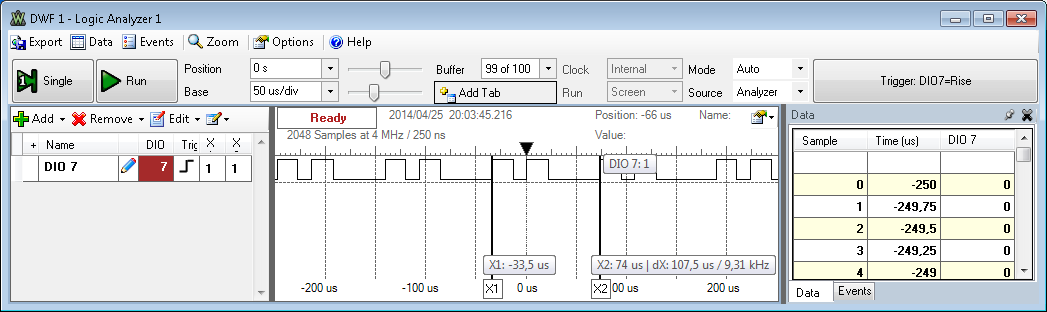
\includegraphics[width=\linewidth]{../src/demo/idle-event-loop-both-manual.png}
  \caption{Minimale activiteit in \'e\'en cyclus van de event loop (manueel)}
  \label{fig:logic-analyser-manual}
\end{figure}

In de figuur zien we deze twee ogenblikken duidelijk naar voor komen. Wanneer
we de doorlooptijd meten van \'e\'en cyclus zien we dat deze rond de 107$\mu$s
ligt. Uit tabel \ref{tbl:manual} weten we dat de gemiddelde doorlooptijd
zonder IDS 48$\mu$s bedraagt. We kunnen concluderen dat, in de manuele
situatie, het toevoegen van een IDS een minimale extra verwerkingstijd met zich
meebrengt van 59$\mu$s of ongeveer 120\%.

Figuur \ref{fig:logic-analyser-generated} toont dezelfde situatie, maar voor de
gegenereerde code. Hier zien we dat er slechts \'e\'en plateau gevormd wordt.
De verwerking van beide algoritmen is in deze situatie gebundeld in de
verwerking door het generatieraamwerk.

\begin{figure}[ht]
  \centering
  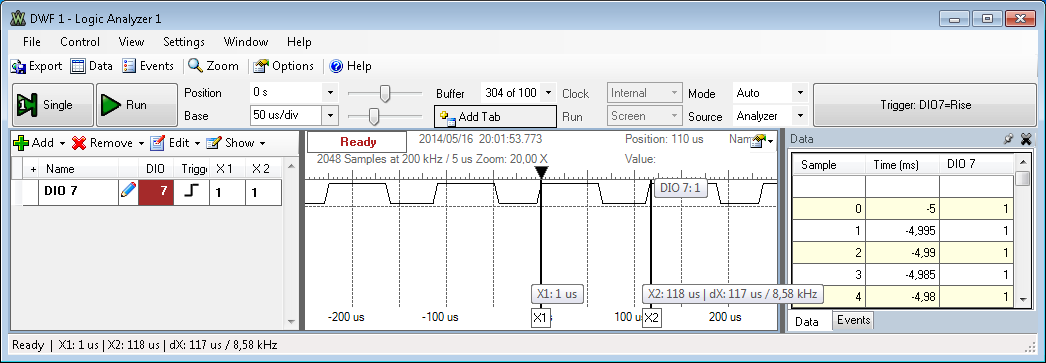
\includegraphics[width=\linewidth]{../src/demo/idle-event-loop-both-generated.png}
  \caption{Minimale activiteit in \'e\'en cyclus van de event loop (gegenereerd)}
  \label{fig:logic-analyser-generated}
\end{figure}

In het geval van de gegenereerde code, zien we dat de doorlooptijd van \'e\'en
cyclus van de event loop zonder speciale activiteit ongeveer 117$\mu$s in
beslag neemt. Dit is 10$\mu$s meer dan bij de manuele implementatie. De
minimale extra verwerkingstijd komt zo op 69$\mu$s of 143\%.

\section{Afsluitende bedenking}

Het is gevaarlijk om een evaluatie van een taal en codegenerator te doen aan de
hand van metingen. De cijfers gepresenteerd in dit hoofdstuk zijn grotendeels
afhankelijk van de beschreven algoritmen, de configuratie, evenals de
feitelijke functionele toepassing. De enige manier waarop deze resultaten
ge\"interpreteerd mogen worden is als een vage bevestiging van wat
logischerwijs reeds ingeschat kon worden, nl. dat men door code beter te
organiseren winst kan boeken.

%!TEX root=masterproef.tex
\chapter{Besluit}
\label{besluit}

\chapterprecishere{
At least for the people who send me mail about a new language that they're
designing, the general advice is: do it to learn about how to write a compiler.
Don't have any expectations that anyone will use it, unless you hook up with
some sort of organization in a position to push it hard. It's a lottery, and
some can buy a lot of the tickets. There are plenty of beautiful languages
(more beautiful than C) that didn't catch on. But someone does win the lottery,
and doing a language at least teaches you something.
\par\raggedleft--- \textup{Dennis Ritchie (1941-2011)},\\
Creator of the C programming language and of UNIX}

% De masterproeftekst wordt afgesloten met een hoofdstuk waarin alle
% besluiten nog eens samengevat worden. Dit is ook de plaats voor suggesties
% naar het verder gebruik van de resultaten, zowel industri\"ele toepassingen
% als verder onderzoek.

\TODO

\section{Sterke punten}
\label{section:strenghts}

\TODO

\section{Zwakke kanten}
\label{section:weaknesses}

\TODO

\section{Opportuniteiten}
\label{section:opportunities}

\TODO

\section{Bedreigingen}
\label{section:threaths}

\TODO

\section{De slotsom}
\label{section:bottom-line}

\TODO

\begin{figure}[ht]
  \centering
  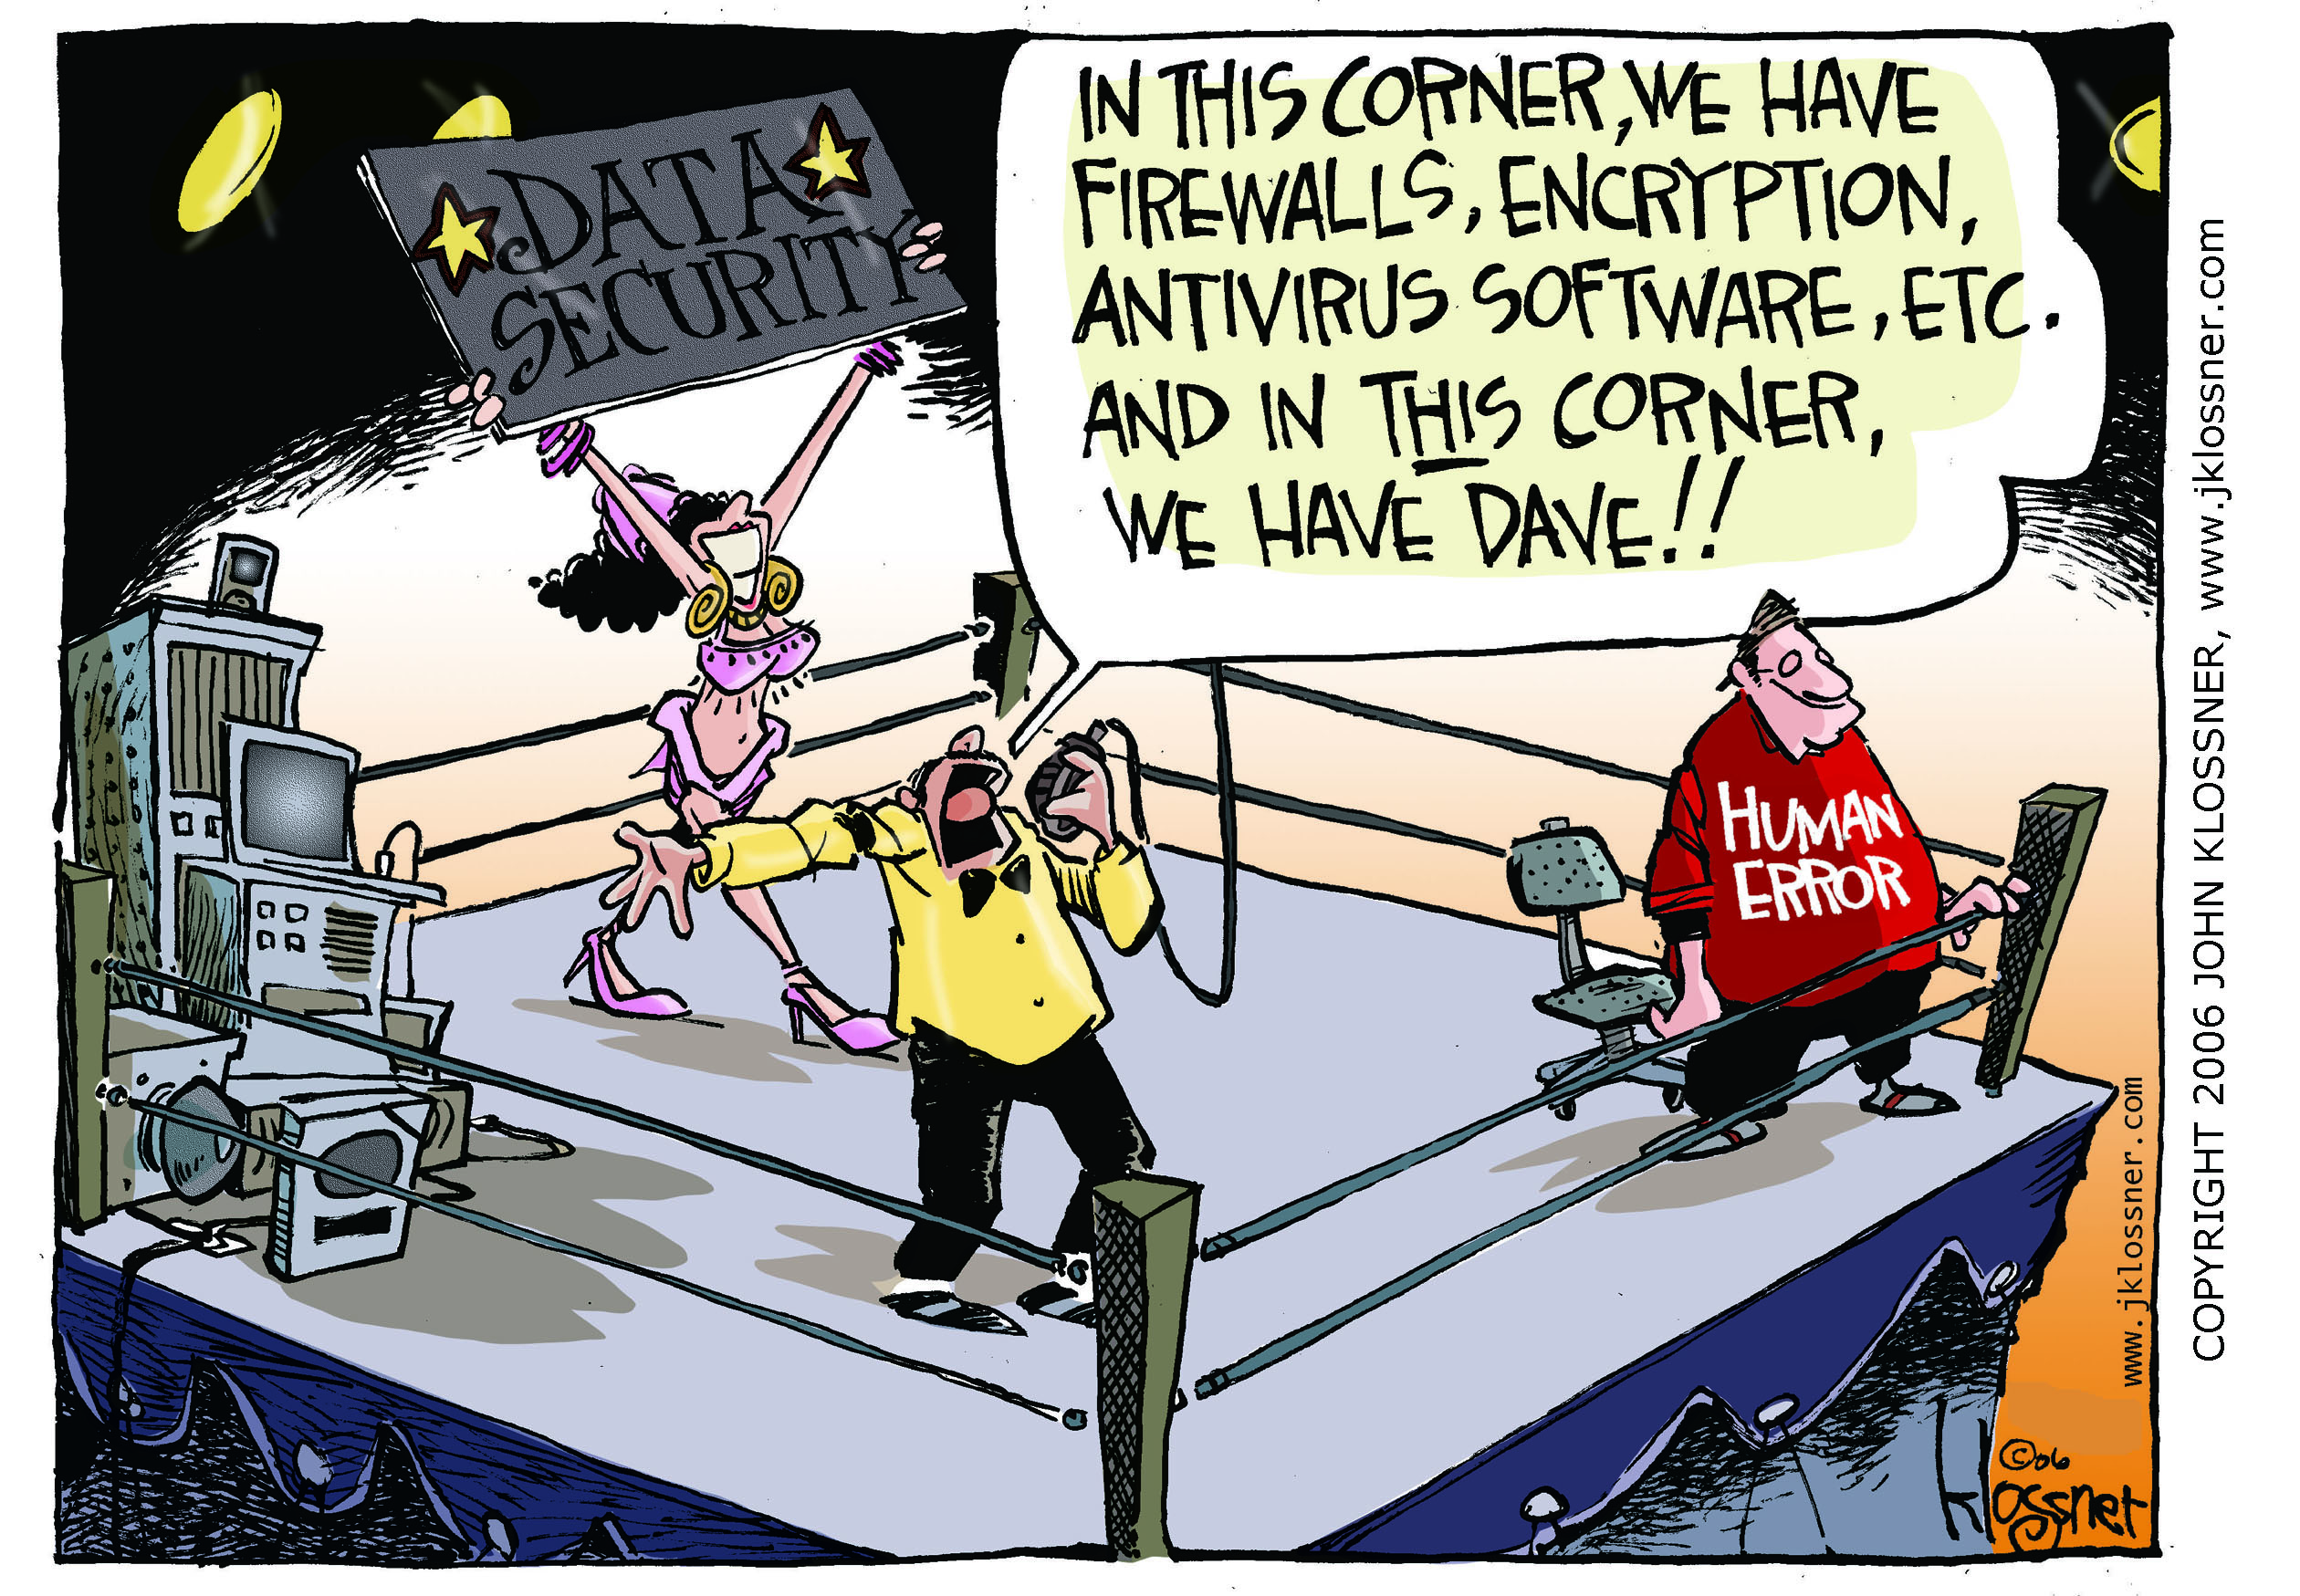
\includegraphics[width=\linewidth]{resources/cartoon_human_error.jpg}
  \caption[``Human Error'']{``Human Error'' - courtesy of John Klossner}
\end{figure}


% TODO:

% Het feit dat in essentie een nieuwe taal was, bracht ook een bijkomende
% leercurve met zich mee. Ook zorgde voortschrijdend inzicht voor stapsgewijze
% verbeteringen aan bepaalde constructies, die echter soms door tijdbeperkingen
% niet voor alle overige code konden bijgewerkt worden.



%!TEX root=masterproef.tex

\chapter*{Nabeschouwing}
\label{nabeschouwing}

In de eerste paragrafen van dit verslag van deze masterproef ben ik de iets wat
ongewone situatie van mijn masterproef niet uit de weg gegaan. Deze laatste
paragrafen wil ik benutten om mijn werk te kaderen en te reflecteren over de
persoonlijke ervaring van de afgelopen maanden.

\begin{quote}
\emph{Het is niet iedereen gegeven om op 40 jarige leeftijd een masterproef te
mogen, of eerder kunnen, maken. De keuze om opnieuw te gaan studeren maak je
niet alleen en vraagt van veel mensen een bijzondere inspanning. Familie en
vrienden, maar ook professoren en assistenten worden plots uit hun vertrouwde
omgeving weggerukt en worden geconfronteerd met een ongewone situatie.}
\end{quote}

Deze ongewone situatie wordt vooral getekend door een voorgeschiedenis met een
reeds uitgebreide ervaring en opgebouwde specialisatie. In mijn geval betreft
het misschien eerder de capaciteit om uitermate generalistische oplossingen te
vinden voor een brede waaier aan informatica-gerelateerde problemen.

Een masterproef is het hoogtepunt van een ingenieursopleiding. Misschien nog
meer dan voor mijn jongere collega's, zou deze opdracht een ware uitdaging
worden om mijn generalistische geest te kaderen in een specialisatie binnen een
zeer sterk afgebakende context. Was ik, na drie jaar, in staat om alle nieuwe
verworven kennis op de juiste manier toe te passen en mij inderdaad master in
het onderwerp te mogen noemen.

Bij aanvang van zowel de voorafgaande studiejaren als de masterproef zelf, had
ik duidelijke een doelstelling om niet zomaar te vervallen in oude gewoontes en
te berusten op mijn ervaring. Mijn masterproef moest inderdaad een duidelijke
ommekeer tonen in mijn manier van denken en moest zonder twijfel getuigen van
een correcte onderzoeksattitude. Daarnaast belichaamde deze hernieuwde
studieperiode de ultieme kans om een herori\"entering van mijn vakgebied te
realiseren.

Met open geest vertrok ik op zoek naar wat mij echt boeide en waar ik mij
effectief meester over wilde maken. Elk vak en elke topic werden onderworpen
aan een diepgaande evaluatie. Elk gesprek met professoren en assistenten peilde
naar mogelijkheden en perspectieven. Elke taak werd beschouwd als een test die
moest uitwijzen of ik er mijn nieuwe toekomst in kon vinden.

Na ongeveer twee jaar was het \emph{moment supr\`eme} aangebroken en moest ik
een keuze maken. Het onderwerp van de masterthesis moest bepaald worden. Tot
mijn ontzetting voelde ik mij er nog helemaal niet klaar voor. Na een
twintigtal vakken en enorm veel informele gesprekken had ik de graal nog niet
gevonden. Geen van de voorgestelde topics konden mijn ogenschijnlijk bekoren en
het was duidelijk dat ik op \'e\'en of andere manier zelf een onderwerp moest
voorstellen.

\'E\'en vakgebied had zich echter van de andere onderscheiden: digitale
electronica en embedded systemen. Dankzij de kennismaking met Professor Hughes
was de wereld van draadloze sensorknopen aan mij ge\"introduceerd en het was
liefde op het eerste gezicht. Misschien was het zelfs geen nieuwe liefde, maar
een liefde die al bestond sinds de vroege jaren tachtig. In een tijdperk waarin
nog amper sprake was van Personal Computers en informatica nog heel dicht stond
bij de electronica die ze implementeerde, zette ik mijn eerste stappen. Reeds
toen voelde ik een grote affiniteit met de zeer elementaire bouwstenen van
computers en de talen die ze konden besturen. De liefde voor compilers is nooit
ver zoek geweest.

Enkele jaren later werd dit, hoofdzakelijk door de intrede van het internet en
niet op zijn minst door de opportuniteit om in \'e\'en van de eerste
internetaanbieders in Antwerpen te mogen helpen, uitgebreid met de mogelijkheid
om systemen met elkaar te verbinden via netwerken. Nog enkele jaren later zou
dit zich nog verder concretiseren tijdens mijn studies aan de KHLeuven en mijn
eerste bedrijfservaringen die volledig in het teken stonden van netwerken en de
beveiliging ervan.

Ofschoon ik mij had voorgenomen om nieuwe terreinen te verkennen, begon alles
toch te wijzen op een enorme samengang van oude en nieuwe liefdes. Met
inbraakdetectie in draadloze sensornetwerken zag ik het huwelijk van
verschillende persoonlijk interesses voltrokken worden.

Net zoals een koppel evolueert na die eerste huwelijksdagen, was mijn
masterproef evenzeer een sterk evoluerende ervaring - zij het dan op een veel
kortere tijdspanne, maar daardoor zeker zo intens. De initi\"ele verwachtingen
maakten snel plaats voor ontzetting en twijfel. Had ik wel de juiste keuze
gemaakt? Had ik wel voldoende vooronderzoek gedaan? Wat als nu deze masterproef
helemaal niet uitdraaide zoals ik mij enkele jaren voordien had voorgenomen?
Had ik ondertussen wel de nodige capaciteiten opgebouwd en was ik wel de
specialist die een masterproef vereist? Of was ik nog steeds dezelfde
generalist, echter nu met wat extra gereedschap in mijn spreekwoordelijke
koffer?

Een antwoord vond ik in de de eigen woorden van de faculteit:
\begin{quote}
\emph{De masterproef wordt beschouwd als een heel belangrijk leermoment in de
ingenieursopleidingen, omdat je als student op een actieve wijze betrokken
wordt bij het onderzoek in het domein waarvoor je gekozen hebt.}
\end{quote}

Het kernwoord voor mij was \emph{onderzoek}; het zoeken betreft hier niet
louter het zoeken naar antwoorden, maar evenzeer naar hypothesen, het zoeken
naar de onderliggende beweegredenen en het durven aanwijzen van problemen.

Ofschoon ik een domein gekozen had en binnen dit domein een deelgebied had
geselecteerd was niet het einde van het defini\"eren van mijn masterproef. Het
onderzoeken van dit domein moest in eerste plaats uitwijzen wat de specifieke
onderzoeksvraag zou zijn die ik op mij durfde te nemen. De ontzetting en angst
die tijdens de eerste weken van literatuurstudie zich had meester gemaakt van
mij, was feitelijk het ontluiken van mijn eigen visie en drijfveer. Plots
kwamen dan ook mijn oude gewoonten opnieuw opzetten.

Net zoals zo vaak tijdens mijn voorgaande professionele carri\`ere was de
ontdekking van de onverwachte chaos en wantoestanden de bron om mijn stoute
schoenen aan te trekken en al mijn ervaring uit de kast te halen om orde op
zaken te scheppen. Het werd snel duidelijk dat het dogmatisch afzweren van mijn
voorgeschiedenis een grove fout zou geweest zijn. Het huwelijk van oude en
nieuwe liefdes, van elementaire informatica en draadloze sensoren werd al snel
ondersteund door software architectuur en code generatie, twee sterke getuigen
uit bijna vervlogen gewaande tijden.

Op dat ogenblik besefte ik dat ik mijn buitengewone situatie dringend moest
omarmen en gebruik moest maken van de unieke kans om mijn oude ervaring en mijn
nieuw verworven kennis te bundelen om een onderwerp te tackelen dat misschien
zelfs iets te groot was voor een \emph{gewone} masterproef.

Het resultaat staat op deze voorgaande bladzijden vereeuwigd. Of het potentieel
dat er in zit ooit ten volle mijn visie zal bereiken zal de toekomst moeten
uitwijzen. Voor mij persoonlijk is deze masterproef een onverdeeld succes. In
het verloop van \'e\'en jaar heb ik al mijn oude ervaring en kennis kunnen en
moeten aanscherpen en mogen verrijken met een enorme nieuwe bagage aan
wetenschappelijke technieken en methoden. Alles wat de afgelopen 30 jaar voor
mij belangrijk is geweest zit vervat in deze masterproef: programmeertalen,
electronica, code generatie, software architectuur, functionele analyse en
eindgebruiker-orientatie,\dots zijn in amper 70 bladzijden samengebracht tot
een resultaat waar ik trots op ben en waar ik hopelijk een nieuw hoofdstuk en
nog vele daarna zal over kunnen schrijven in de nabije toekomst.

\bigskip

Dank aan allen die dit mogelijk hebben gemaakt.\\
Ja, jullie allemaal.


\appendixpage*
\appendix
%!TEX root=masterproef.tex

\chapter{FOO-lang grammatica}
\label{appendix:foo-lang-grammar}

\begin{verbatim}
start    ::= modules? EOF
modules  ::= module*
module   ::= 'module' identifier instructions?
instructions
         ::= instruction*
instruction
         ::= declaration
           | directive
           | extension
declaration
         ::= annotated_declaration
           | constant_declaration
           | event_handler_declaration
           | function_declaration
annotated_declaration
         ::= annotation apply_declaration
           | annotation function_declaration
annotation
         ::= '@' function_call_expression
apply_declaration
         ::= 'with' scoping 'do' function_expression
constant_declaration
         ::= 'const' name_type_value
event_handler_declaration
         ::= event_timing scoping function_expression 'do' function_expression
scoping  ::= domain '.' identifier
           | domain
domain   ::= identifier
event_timing
         ::= 'before'
           | 'after'
function_prototype
         ::= identifier '(' function_param_type_list? ')' ':' type
function_param_type_list
         ::= type ( ',' type )*
function_declaration
         ::= 'function' identifier '(' function_param_list? ')' function_body
function_expression
         ::= 'function' identifier? '(' function_param_list? ')' function_body
           | identifier
function_param_list
         ::= identifier ( ',' identifier )*
function_body
         ::= block_statement
statements
         ::= statement*
statement
         ::= block_statement
           | assignment_statement
           | increment_statement
           | decrement_statement
           | if_statement
           | case_statement
           | call_expression
           | 'return'
block_statement
         ::= '{' '}'
           | '{' statement+ '}'
assignment_statement
         ::= variable_expression ( '=' | '+=' | '-=' ) expression
increment_statement
         ::= variable_expression '++'
decrement_statement
         ::= variable_expression '--'
if_statement
         ::= 'if' '(' expression ')' statement 'else' statement
           | 'if' '(' expression ')' statement
case_statement
         ::= 'case' expression '{' case_clauses? '}'
case_clauses
         ::= case_clause*
case_clause
         ::= function_call_expression block_statement
           | 'else' statement
expression
         ::= logical_expression
logical_expression
         ::= or_expression
or_expression
         ::= and_expression ( 'or' and_expression )*
and_expression
         ::= equality_expression ( 'and' equality_expression )*
equality_expression
         ::= order_expression ( ( '==' | '!=' ) order_expression )*
order_expression
         ::= additive_expression ( ( '<' | '<=' | '>' | '>=' ) additive_expression )*
additive_expression
         ::= multiplicative_expression ( ( '+' | '-' ) multiplicative_expression )*
multiplicative_expression
         ::= unary_expression ( ( '*' | '/' | '%' ) unary_expression )*
unary_expression
         ::= '!'? primary_expression
primary_expression
         ::= '(' logical_expression ')'
           | literal
           | call_expression
           | variable_expression
           | atom
           | matching_expression
call_expression
         ::= method_call_expression
           | function_call_expression
method_call_expression
         ::= object_expression '.' function_call_expression
function_call_expression
         ::= identifier '(' argument_list? ')'
argument_list
         ::= expression ( ',' expression )*
variable_expression
         ::= property_expression
           | identifier ':' type
           | identifier
property_expression
         ::= object_expression '.' identifier
object_expression
         ::= identifier '.' identifier
           | identifier
           | object_literal
directive
         ::= import_directive
import_directive
         ::= 'from' identifier 'import' function_prototype
extension
         ::= 'extend' domain 'with' object_literal
literal  ::= numeric_literal
           | boolean_literal
           | object_literal
           | list_literal
boolean_literal
         ::= 'true'
           | 'false'
numeric_literal
         ::= INTEGER
           | FLOAT
object_literal
         ::= '{' property_literal_list? '}'
property_literal_list
         ::= property_literal property_literal*
property_literal
         ::= name_type_exp
name_type_value
         ::= identifier optional_type '=' literal
name_type_exp
         ::= identifier optional_type '=' expression
optional_type
         ::= ':' type
           |
atom     ::= '#' identifier
matching_expression
         ::= dontcare
           | comparison
dontcare ::= '_'
comparison
         ::= comparator expression
comparator
         ::= '<'
           | '<='
           | '>'
           | '>='
           | '=='
           | '!='
           | '!'
list_literal
         ::= '[' ']'
           | '[' expression ( ',' expression )* ']'
type     ::= amount_type
           | many_type '*'
           | many_type
           | basic_type
           | tuple_type '*'
           | tuple_type
many_type
         ::= basic_type '*'
basic_type
         ::= type_identifier
type_identifier
         ::= 'byte'
           | 'integer'
           | 'float'
           | 'boolean'
           | 'timestamp'
           | identifier
tuple_type
         ::= '[' type ( ',' type )* ']'
amount_type
         ::= basic_type '[' INTEGER ']'
identifier
         ::= ID
           | 'from'
           | 'import'
           | 'with'
           | 'use'
           | 'extend'
_        ::= COMMENT
           | WS

<?TOKENS?>

INTEGER  ::= '0'
           | [1-9] [0-9]*
FLOAT    ::= [0-9]+ '.' [0-9]*
ID       ::= ( [a-z] | [A-Z] | '_' ) ( [a-z] | [A-Z] | '_' | [0-9] )*
COMMENT? ::= '//' [^#xA#xD]* #xD? #xA
           | '/*' .* '*/'
WS       ::= ' '
           | #x9
           | #xD
           | #xA
EOF      ::= $
\end{verbatim}

%!TEX root=masterproef.tex

\chapter{C code voor \ttt{hello.foo}}
\label{appendix:hello-srcs}

Deze bijlage bevat de belangrijkste gegenereerde code van \ttt{hello.foo},
ge\"introduceerd in hoofdstuk \ref{chapter:implementatie}.

\section{main.c}
\vspace{-5mm}
\begin{listing}[H]
  \begin{minted}[linenos,frame=lines,framesep=2mm,fontsize=\footnotesize]{c}
#include "main.h"
//  init and application_step
void init(void) {
  // add framework init here
  nodes_init();
  mesh_on_receive(payload_parser_parse);
}
void application_step(void) {
  // add application specific code here
}
/*
  starting point
  please don't change anything beyond this point.
*/
int main(void) {
  init();
  nodes_scheduler_init();
  while(TRUE) {
    // your application gets its share
    application_step();
    // nodes logic execution hook
    nodes_process();
    xbee_receive();
  }
  return 1;
}
void nodes_scheduler_init(void) {
  nodes_schedule_all(interval, step);
}
  \end{minted}
  \vspace{-5mm}
  \caption{Generatie van \ttt{hello.foo}: main.c}
\end{listing}

\section{constants.h}
\vspace{-5mm}
\begin{listing}[H]
  \begin{minted}[linenos,frame=lines,framesep=2mm,fontsize=\footnotesize]{c}
#ifndef __CONSTANTS_H
#define __CONSTANTS_H

#define interval 1000

#endif
  \end{minted}
  \vspace{-5mm}
  \caption{Generatie van \ttt{hello.foo}: constants.h}
\end{listing}

\section{node\_t.h}
\vspace{-5mm}
\begin{listing}[H]
  \begin{minted}[linenos,frame=lines,framesep=2mm,fontsize=\footnotesize]{c}
#ifndef __NODE_T_H
#define __NODE_T_H

#include "moose/bool.h"
// THE node type
typedef struct node_t {
  // domain properties
  uint8_t id;
  uint16_t address;
  // extended properties for hello
  uint8_t sequence;
} node_t;
void init_node(node_t* node);

#endif
  \end{minted}
  \vspace{-5mm}
  \caption{Generatie van \ttt{hello.foo}: node\_t.h}
\end{listing}

\section{node\_t.c}
\vspace{-5mm}
\begin{listing}[H]
  \begin{minted}[linenos,frame=lines,framesep=2mm,fontsize=\footnotesize]{c}
#include "node_t.h"
void init_node(node_t* node) {
  node->sequence = 0;
}
  \end{minted}
  \vspace{-5mm}
  \caption{Generatie van \ttt{hello.foo}: node\_t.c}
\end{listing}

\section{nodes-hello.h}
\vspace{-5mm}
\begin{listing}[H]
  \begin{minted}[linenos,frame=lines,framesep=2mm,fontsize=\footnotesize]{c}
#ifndef __NODES_HELLO_H
#define __NODES_HELLO_H

#include "nodes.h"
#include "includes.h"
void step(node_t* node);

#endif
  \end{minted}
  \vspace{-5mm}
  \caption{Generatie van \ttt{hello.foo}: nodes-hello.h}
\end{listing}

\section{nodes-hello.c}
\vspace{-5mm}
\begin{listing}[H]
  \begin{minted}[linenos,frame=lines,framesep=2mm,fontsize=\footnotesize]{c}
#include "nodes-hello.h"
void step(node_t* node) {
  if((node->sequence < 10)) {
    node->sequence++;
  }
}
  \end{minted}
  \vspace{-5mm}
  \caption{Generatie van \ttt{hello.foo}: nodes-hello.c}
\end{listing}

%!TEX root=masterproef.tex

\chapter{Hardwareplatform}
\label{hardware-platform}

Voor het hardwareplatform werd gekozen om niet te vertrekken van een bestaand
platform, zoals Arduino \citep{url:arduino} of Atmel RZRaven
\citep{manual:rzraven}. Wel werd geopteerd om te vertrekken van elementaire
componenten: een Atmel ATMEGA1284p \mcu \citep{datasheet:atmega1284p}, een Digi
XBee-module \citep{manual:xbee} en een MAX232 seri\"ele driver-module
\citep{datasheet:max232}.

De beweegreden vindt zijn oorsprong in het aspect betreffende
\emph{standaardisatie} uit de probleemdefinitie (zie sectie
\ref{section:problem-definition}). De keuze van elementaire bouwstenen
reduceert het hardwareplatform tot zijn essentie. De implementatie van de
oplossing kan immers geen gebruik maken van specifieke voorzieningen en dient
alle functionaliteit zelf te voorzien.

Hierdoor is een prototype, gebaseerd op dit platform, representatief voor het
eenvoudigste platform en zal elke toevoeging in de vorm van een uitgebreider
hardwareplatform, slechts meer stabiliteit en mogelijkheden bieden, die de
ontwikkeling louter positief kunnen be\"invloeden.

\section{Minimale noden en voorzieningen}

We overlopen kort de noden en hoe deze voorzien zijn in het platform:

\begin{description}

  \item[Rekenkracht en geheugen] De Atmel ATMEGA1284p is een veelgebruikte
  \mcu. We vinden hem o.a. terug in de populaire Atmel RZRaven ontwikkelingskit
  en op veelgebruikte versies van het Arduino-platform. Hij beschikt over 128KB
  programmeerbaar geheugen en 16KB werkgeheugen. Daarnaast beschikt deze \mcu
  over twee USART seri\"ele poorten.
  
  \item[Draadloos netwerk] \'E\'en van deze poorten kan gebruikt worden voor de
  aansturing van de Digi XBee-module. Deze module biedt met een eenvoudige
  seri\"ele interface toegang tot een ZigBee-netwerk. De eenvoudige interface
  laat toe om bytes te versturen en te ontvangen en implementeert een minimale
  ondersteuning voor het ZigBee-protocol.
  
  \item[Communicatie] Om in parallel met het draadloze netwerk te kunnen
  communiceren met een computer en zo bijkomende informatie te kunnen weergeven
  betreffende de werking van de implementatie, is een MAX232 seri\"ele
  driver-module voorzien. Deze laat toe om via een seri\"ele verbinding en een
  terminal een byte-geori\"enteerde communicatie te realiseren.
  
  \item[Indicatoren] Enkele LEDs (\emph{Light Emitting Diode}) geven
  elementaire feedback over de werking van het ontwerp. Een rode LED geeft aan
  dat het platform onder spanning staat en twee LEDs, oranje en geel, geven
  respectievelijk de beschikbaarheid van het draadloze netwerk en de
  operationele status van de XBee-module aan.
  
\end{description}

\section{Ontwerp}

Figuur \ref{fig:hardware-platform-schematic} toont het schema van het platform.

\begin{figure}[ht]
  \centering
  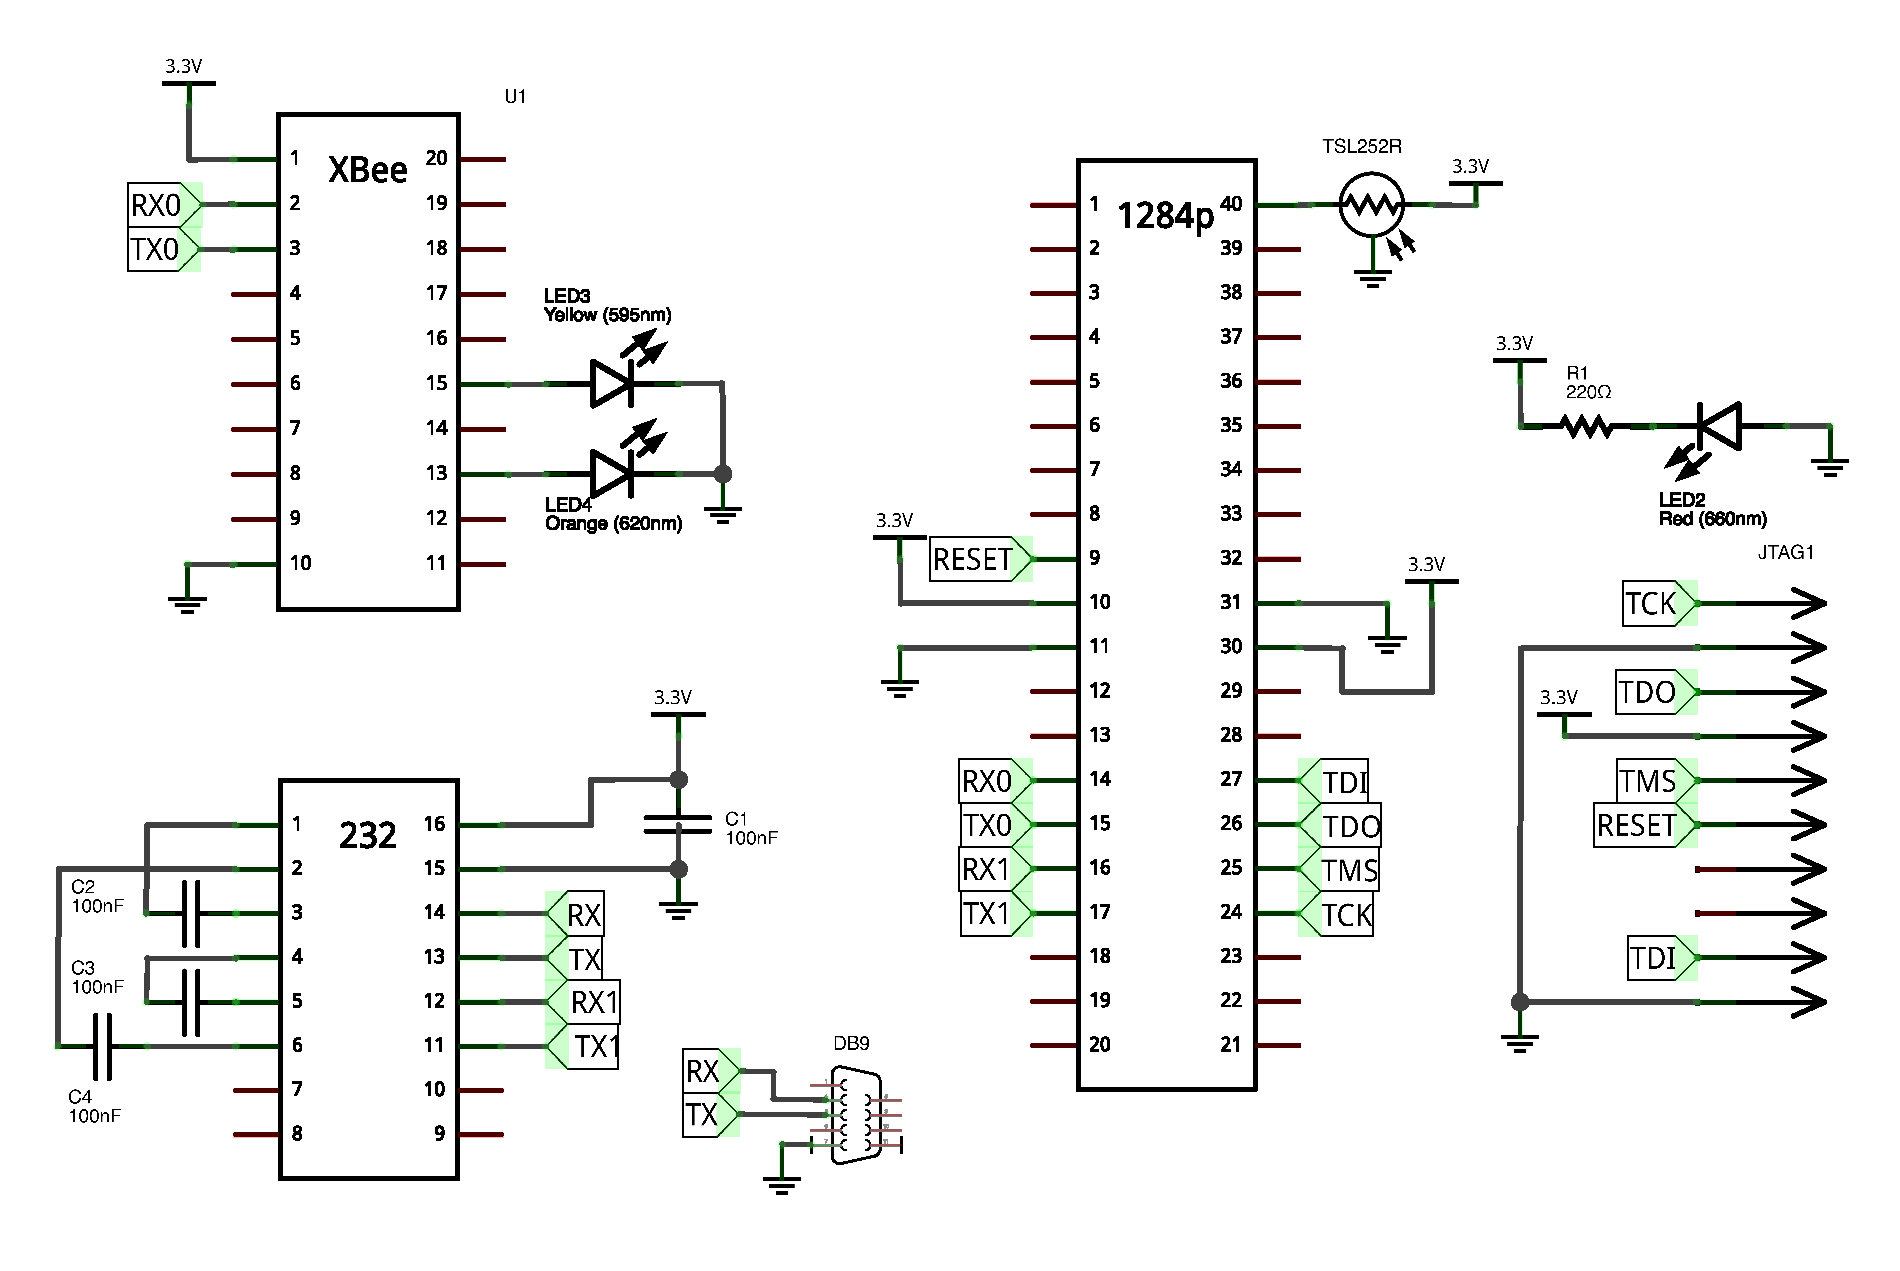
\includegraphics[width=\linewidth]{resources/hardware-platform-schematic.pdf}
  \caption{Schema van hardwareplatform}
  \label{fig:hardware-platform-schematic}
\end{figure}

Op het schema herkennen we de verschillende componenten: centraal de
ATMEGA1284p, met rechts bovenaan de lichtsensor (TSL252R). Rechts daarvan is de
rode LED indicator en de JTAG aansluiting weergegeven. Links bovenaan vinden we
de XBee-module met twee indicatoren en twee seri\"ele verbindingen voor het
versturen en ontvangen van bytes. Tot slot is er links onderaan de
MAX232-module, met verbindingen naar de tweede USART en een DB9-connector.

%!TEX root=masterproef.tex

\chapter{Simulatie van routering voor een XBee-gebaseerd maasnetwerk}
\label{virtual-mesh}

Het hardwareplatform, beschreven in \ref{hardware-platform}, beschikt over een
XBee module om het ZigBee netwerk op te bouwen. Deze module biedt een zeer
hoogniveau interface aan, waardoor alle routering en andere lagerniveau
concepten verborgen blijven. Zo is het bv. onmogelijk om communicatie die niet
voor de eigen radio bestemd is op te vangen, terwijl dit net een typische
eigenschap is van een draadloos (maas)netwerk.

Aangezien het kunnen opvolgen van het verder doorsturen van berichten een
belangrijk aspect is en hiervoor alle communicatie die opgevangen kan worden
ter beschikking moet staan van het algoritme, was het nodig om dit gedrag na te
bootsen om een realistische demonstratie van de algoritmen mogelijk te maken.

Hiertoe werd een virtuele routering ge\"implementeerd. Deze maakt het mogelijk
om aan de hand van \emph{broadcast} berichten en extra informatie omtrent de
oorspronkelijke zender en eventuele tussenliggende knopen, alle mogelijkheden
van een volledig toegankelijk ZigBee netwerk te simuleren.

\section{Opstelling}

Figuur \ref{fig:xbee-setup} toont de opstelling voor de demonstratie: drie XBee
modules zijn geconfigureerd als een eind-knoop, een router en een
co\"ordinator. De co\"ordinator is via een \emph{explorerboard} verbonden met
een computer. Op deze manier is het mogelijk om deze XBee module te benaderen
aan de hand van een seri\"ele verbinding. De eind-knoop en de router zijn twee
identieke sensorknopen.

\begin{figure}[ht]
  \centering
  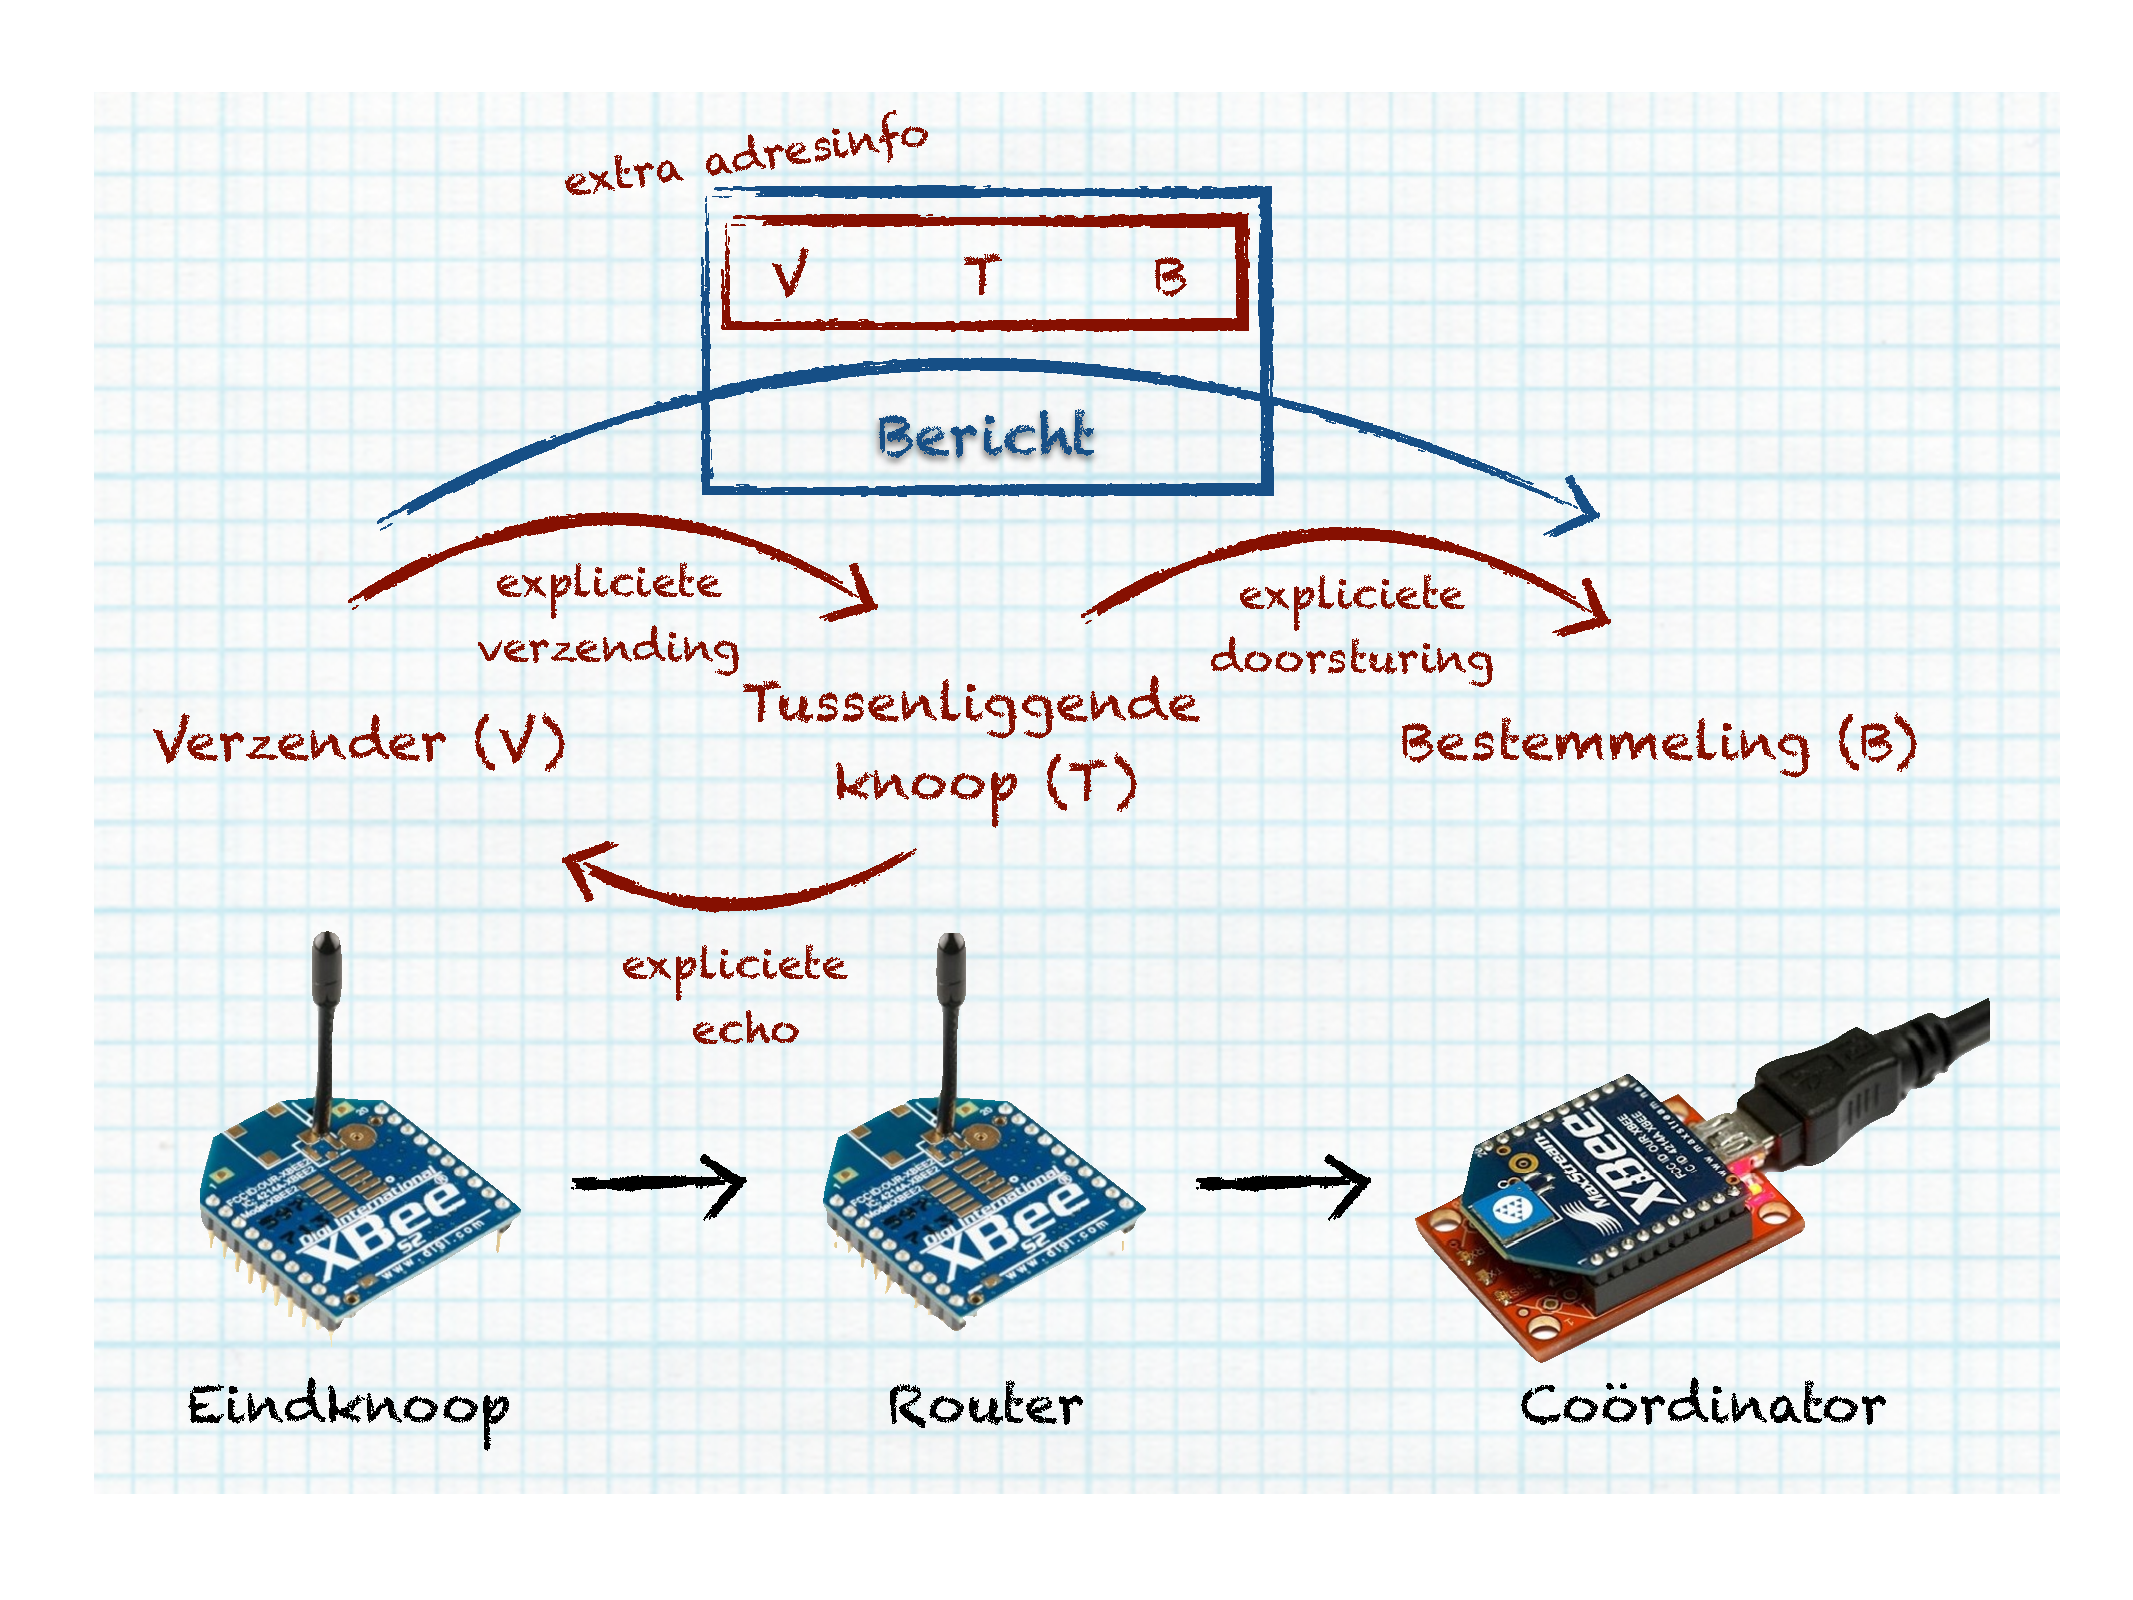
\includegraphics[width=\linewidth]{resources/xbee-setup.pdf}
  \caption{Opstelling van maasnetwerk voor demonstratie.}
  \label{fig:xbee-setup}
\end{figure}

Om met de drie XBee modules op een correcte manier tot een maasnetwerk te
komen, moeten we de modules voorzien van een specifieke configuratie. Zo wordt
bij de co\"rdinator de tijdspanne dat nieuwe knopen het netwerk kunnen
vervoegen beperkt tot \'e\'en minuut. Dit gebeurt aan de hand van het \ttt{NJ}
(Node Join) commando. Gedurende deze periode kan dan de router geactiveerd
worden. Na associatie van deze radio en het verstrijken van de minuut, kan dan
de eind-knoop geactiveerd worden. Deze zal niet meer rechtstreeks bij de
co\"ordinator kunnen aansluiten en zal via de router het netwerk moeten
benaderen.

\section{Doorsturen van berichten}

Een tweede aanpassing die dient doorgevoerd te worden, is de manier waarop de
router berichten van de eind-knoop verder doorstuurt naar de co\"ordinator.
Indien we dit door de standaard netwerkvoorzieningen van de XBee module zouden
later doen, zouden we deze berichten opnieuw niet kunnen onderscheppen. We
moeten deze daarom zelf \emph{manueel} doorsturen.

Bij het versturen van berichten worden tevens drie bijkomende netwerk adressen
van de betrokken knopen toegevoegd aan het feitelijke bericht: het adres van de
oorspronkelijke verzender, het adres van de tussenliggende knoop en het adres
van de uiteindelijke bestemmeling. Dit stelt ons functioneel in staat om
voldoende informatie te hebben om berichten van andere knopen onderling te
interpreteren.

De extra code die deze simulatie realiseert is weergegeven in listing
\ref{lst:virtual-mesh}. Ze volgt de opbouw van de overeenkomstige code voor
normale aansturing van de XBee module: een verzend functie, een ontvang functie
en de mogelijkheid om een externe verwerker voor binnenkomende berichten te
registreren.

De werking wordt duidelijk aan de hand van een voorbeeld, waarbij zowel de
eind-knoop als de router een bericht verzenden naar de co\"ordinator. De
uitvoer van deze demonstratie is weergegeven in figuur \ref{fig:virtual-mesh}:
van boven naar onder zien we de uitvier van de eind-knoop, de router en de
co\"ordinator.

Zowel de eind-knoop als de router gebruiken exact dezelfde code. Na het
initialiseren van de seri\"ele verbinding en het opzetten van de
netwerkassociatie, tonen beide knopen eerst hun eigen netwerk adres en dat van
hun hi\"erarchisch ouderlijke knoop (Engels: \emph{parent}). In dit geval heeft
de eind-knoop netwerk adres \ttt{4d 83} en de router adres \ttt{fa 7d}. We zien
dat de eind-knoop inderdaad als \emph{parent} de router opgeeft.

De router geeft als \emph{parent} \ttt{ff fe} aan. Dit adres staat voor een
onbekend adres. XBee routers geven dit adres standaard terug aangezien het
\emph{parent} concept voor hen niet bestaat. 

\inputminted[linenos,frame=lines,framesep=2mm,fontsize=\footnotesize,firstline=39, firstnumber=39]{c}{../src/demo/lib/network.c}
\vspace{-5mm}
\captionof{listing}{Simulatie van een maasnetwerk met XBee modules.
\label{lst:virtual-mesh}}
\vspace{3mm}

In deze beperkte simulatieopstelling kunnen we dit adres gelijkstellen aan het
adres van de co\"ordinator: \ttt{00 00}.

De router zal na associatie met het netwerk, gedurende 20 seconden wachten,
alvorens zijn eigen bericht te versturen. Gedurende deze tijd kunnen we de
eind-knoop activeren. Tijdens het wachten, verwerkt de router wel binnenkomende
berichten. Zoals we kunnen zien was de eind-knoop reeds verbonden met het
netwerk via de router na een 18tal seconden. De router ontving het bericht van
de eind-knoop en besliste op basis van de uiteindelijke bestemming om het
bericht verder te versturen. Dit expliciet doorgestuurde bericht komt zowel toe
bij de co\"ordinator als de eind-knoop.

Tot slot, verstuurt ook de router een bericht naar de co\"ordinator. Opnieuw
ontvangen zowel de co\"ordinator als de eind-knoop dit bericht.

\begin{figure}[ht]
\centering
\begin{subfigure}{.67\linewidth}
  \centering
  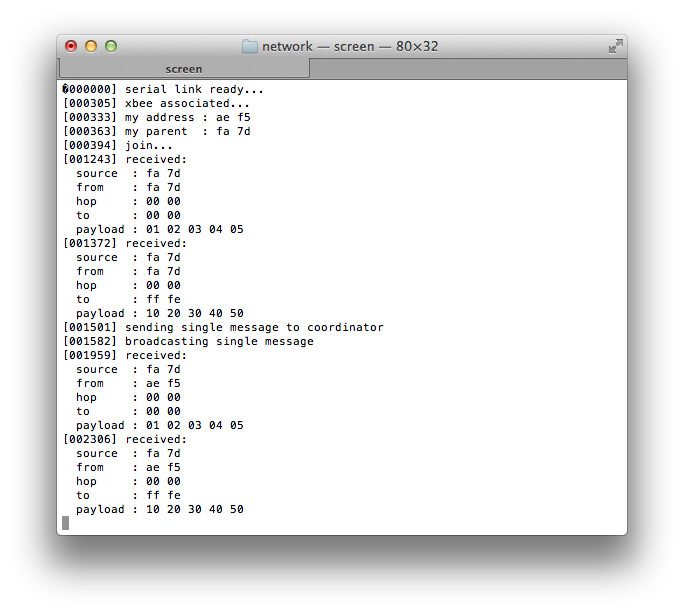
\includegraphics[width=.9\linewidth]{../src/demo/network/end-device.png}
  \caption{Eind-knoop}
  \label{fig:virtual-mesh-end-device}
\end{subfigure}
\begin{subfigure}{.67\linewidth}
  \centering
  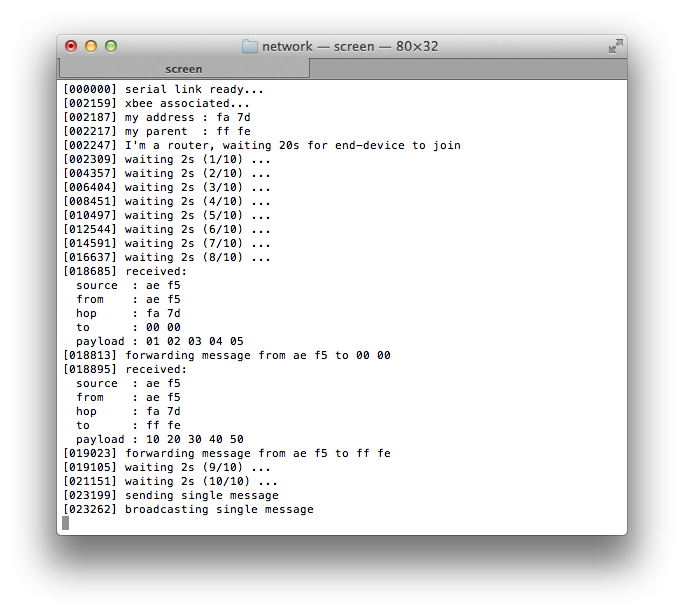
\includegraphics[width=.9\linewidth]{../src/demo/network/router.png}
  \caption{Router}
  \label{fig:virtual-mesh-router}
\end{subfigure}
\begin{subfigure}{.67\linewidth}
  \centering
  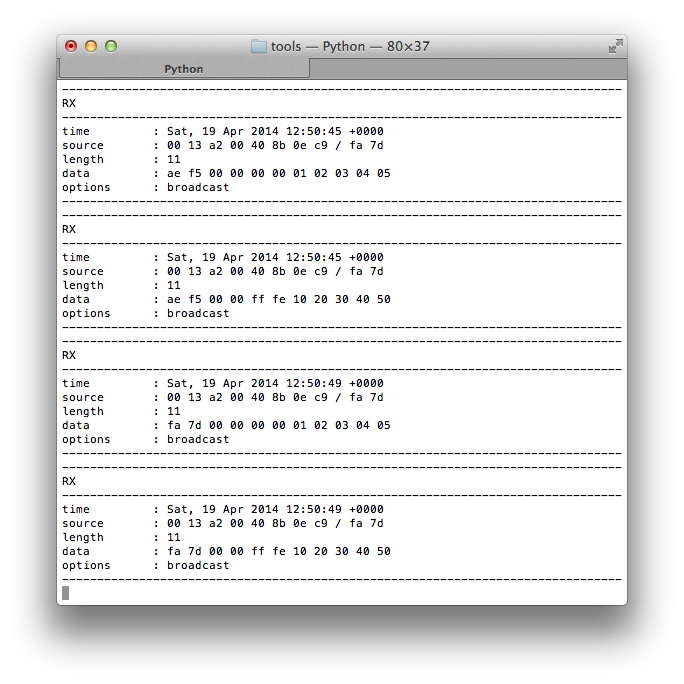
\includegraphics[width=.9\linewidth]{../src/demo/network/coordinator.png}
  \caption{Coordinator}
  \label{fig:virtual-mesh-coordinator}
\end{subfigure}
\caption{Simulatie van een maasnetwerk op basis van XBee modules.}
\label{fig:virtual-mesh-output}
\end{figure}

%!TEX root=masterproef.tex

\chapter{FOO-lang broncode van selectie detectiealgoritmen}
\label{appendix:demo-code}

De in FOO-lang beschreven voorbeelden van detectiealgoritmen vormen de basis
voor de evaluatie van het prototype dat in deze masterproef ge\"implementeerd
werd.

\section{\emph{Heartbeat}}
\label{section:demo-code-heartbeat}

\inputminted[linenos,frame=lines,framesep=2mm,fontsize=\footnotesize]{js}{../src/foo-lang/examples/heartbeat.foo}
\vspace{-5mm}
\captionof{listing}{\ttt{heartbeat.foo}
  \label{lst:heartbeat.foo}}

\section{Reputatie}
\label{section:demo-code-reputation}

\inputminted[linenos,frame=lines,framesep=2mm,fontsize=\footnotesize]{js}{../src/foo-lang/examples/reputation.foo}
\vspace{-5mm}
\captionof{listing}{\ttt{reputation.foo}
  \label{lst:reputation.foo}}

\section{Samenwerking}
\label{section:demo-code-cooperation}

De volgende FOO-lang broncode is een experimenteel document dat diende als
oefening om na te gaan hoeveel aanpassingen aan FOO-lang zouden moeten gebeuren
om een derde algoritme te kunnen beschrijven.

De broncode bevat aanwijzingen naar en bedenkingen omtrent bepaalde
oplossingen. Veel van de opmerkingen hebben betrekking op de implementatie van
de code generator. Slechts een minderheid aan echte aanpassingen noodzaken een
wijziging aan FOO-lang.

\inputminted[linenos,frame=lines,framesep=2mm,fontsize=\footnotesize]{js}{../src/foo-lang/examples/cooperation.foo}
\vspace{-5mm}
\captionof{listing}{\ttt{cooperation.foo}
  \label{lst:cooperation.foo}}


\backmatter

\bibliographystyle{plainnat}
\bibliography{referenties}

\end{document}
